\section{Revisión de la Literatura}
\label{sec:revision_literatura}

% Introducción breve al capítulo de estado del arte (1 párrafo)

% Bloque 2.1: Fundamentos Matemáticos de los Embeddings y Espacios Latentes (Págs. 1-5)
% =============================================================================
% CAPÍTULO 2 - BLOQUE 2.1: FUNDAMENTOS MATEMÁTICOS DE LOS EMBEDDINGS,
% ESPACIOS LATENTES CONTINUOS Y SUPERACIÓN DEL PARADIGMA OCR
% =============================================================================

\subsection{Fundamentos Matemáticos de los Embeddings Multimodales y Espacios Semánticos Continuos}
\label{subsec:fundamentos_embeddings}

\subsubsection{El Problema del Análisis Secuencial y la Representación de Datos No Estructurados}
\label{subsubsec:problema_analisis_secuencial}

El crecimiento sostenido de los repositorios multimedia en entornos académicos, industriales y de radiodifusión ha puesto de manifiesto un problema metodológico fundamental en la ingeniería de datos: la extrema ineficiencia del análisis secuencial humano frente a volúmenes masivos de información no estructurada \cite{prajwal2025multimodal}. Históricamente, la tarea de localizar un evento singular dentro de un archivo de vídeo de larga duración (disciplina denominada en la literatura científica como \textit{Long-form Video Understanding} o \textit{Video RAG}) exigía bien un visionado manual exhaustivo por parte de operadores humanos, o bien una dependencia absoluta de metadatos descriptivos y etiquetas manuales generadas previamente a la indexación \cite{multi_rag2025}. En escenarios reales que abarcan desde archivos históricos de televisión y auditorías de videovigilancia hasta repositorios de clases universitarias grabadas o historiales médicos complejos, el etiquetado manual resulta técnica y económicamente inviable.

Para superar la barrera del procesamiento manual, los sistemas de Recuperación de Información (\textit{Information Retrieval}) evolucionaron hacia el paradigma de la Recuperación Aumentada por Generación (RAG, por sus siglas en inglés) \cite{prajwal2025multimodal}. No obstante, mientras que las arquitecturas RAG de primera generación operaban exclusivamente sobre cadenas de texto plano, los flujos multimedia contemporáneos requieren procesar, alinear e interpretar simultáneamente señales heterogéneas compuestas por secuencias de fotogramas, pistas de audio y texto libre \cite{prajwal2025multimodal, multi_rag2025}.

La base matemática que permite a un sistema computacional operar sobre formatos tan dispares sin recurrir a reglas heurísticas manuales es el concepto de \textbf{representación vectorial densa} o \textbf{\textit{embedding}} \cite{gemini_emb2_docs}. Un \textit{embedding} es una proyección matemática que transforma un objeto de entrada arbitrario $x$ (ya sea una oración en lenguaje natural, una matriz de píxeles correspondiente a un fotograma de vídeo o una onda acústica) en un vector de números reales en coma flotante $\mathbf{v} \in \mathbb{R}^d$ dentro de un espacio métrico continuo de dimensión $d$, según se formaliza en la Ecuación~\eqref{eq:proyeccion_multimodal} \cite{gemini_emb2_docs}:

\begin{equation}
f_{\theta}: \mathcal{X}_{\text{texto}} \cup \mathcal{X}_{\text{imagen}} \cup \mathcal{X}_{\text{vídeo}} \cup \mathcal{X}_{\text{audio}} \cup \mathcal{X}_{\text{PDF}} \longrightarrow \mathbb{R}^d
\label{eq:proyeccion_multimodal}
\end{equation}

donde $f_{\theta}$ representa una red neuronal profunda parametrizada por los pesos $\theta$ (un Modelo Fundacional Multimodal) y $\mathbb{R}^d$ constituye el \textbf{espacio semántico compartido} o espacio latente unificado \cite{gemini_emb2_docs}. La propiedad fundamental de este mapeo unificado reside en que la topología del espacio vectorial preserva la semántica subyacente con independencia de la modalidad de origen: para que un sistema inteligente comprenda que la fotografía de un objeto o ser vivo (por ejemplo, la imagen de un perro), su manifestación acústica (el ladrido grabado en una pista de audio) y su representación simbólica (la palabra escrita ``perro'') expresan el mismo concepto, el modelo proyecta las tres entradas hacia coordenadas geométricas sumamente próximas entre sí dentro del mismo plano matemático \cite{gemini_emb2_docs}.

\subsubsection{El Ocaso de las Canalizaciones OCR y la Ingestión Visual Nativa con M-RoPE}
\label{subsubsec:ocaso_ocr_mrope}

Durante la primera mitad de la década de 2020, el diseño estándar para indexar contenido visual y de vídeo en sistemas RAG imponía una canalización rígida, escalonada y unimodal \cite{prajwal2025multimodal}. Este flujo tradicional obligaba a extraer fotogramas aislados del vídeo, aplicar algoritmos clásicos de detección de contornos, someter cada imagen a un motor de Reconocimiento Óptico de Caracteres (OCR) para obtener cadenas de texto plano, transcribir en paralelo la pista de audio mediante sistemas de Reconocimiento Automático del Habla (ASR, como el modelo Whisper) e inyectar finalmente todo el texto concatenado en un modelo de \textit{embeddings} puramente textual \cite{prajwal2025multimodal, video_rag2024}.

La literatura científica publicada entre 2024 y 2026 ha demostrado empíricamente el colapso operativo de este paradigma basado en traducción forzosa a texto plano \cite{prajwal2025multimodal}. Convertir toda la riqueza de una señal visual en secuencias léxicas mediante OCR introduce tres deficiencias estructurales críticas \cite{prajwal2025multimodal}:
\begin{enumerate}
    \item \textbf{Cuello de botella informacional:} La traducción de una escena tridimensional o de un fotograma complejo a palabras sueltas descarta toda la información visual no textual, tales como acciones físicas, colores, texturas, expresiones emocionales e interacciones implícitas entre objetos \cite{prajwal2025multimodal}.
    \item \textbf{Destrucción del diseño espacial (\textit{Layout}):} Cuando un sistema procesa diapositivas académicas, diagramas arquitectónicos, tablas financieras o editores de código fuente extrayendo únicamente los caracteres visibles mediante OCR, la disposición bidimensional (\textit{layout}) y las relaciones jerárquicas y topológicas entre los bloques visuales desaparecen por completo \cite{prajwal2025multimodal}.
    \item \textbf{Propagación de errores en cascada:} Cualquier fallo de reconocimiento en el motor OCR (frecuente ante cambios de iluminación, tipografías pequeñas, compresión de vídeo o fondos oscuros) corrompe irreversiblemente el texto indexado, impidiendo que el motor de búsqueda recupere el segmento aunque el contenido visual original sea perfectamente claro para un observador \cite{prajwal2025multimodal}.
\end{enumerate}

La Figura~\ref{fig:ocr_vs_multimodal} contrasta esquemáticamente el flujo tradicional dependiente de OCR frente al paradigma contemporáneo de vectorización multimodal directa \cite{prajwal2025multimodal}.

\begin{figure}[htbp]
\centering
\begin{tikzpicture}[
    node distance=0.8cm and 1.0cm,
    box/.style={rectangle, draw=black!80, fill=gray!10, thick, minimum width=2.4cm, minimum height=0.9cm, align=center, font=\footnotesize, rounded corners=2pt},
    badbox/.style={rectangle, draw=red!80!black, fill=red!8, thick, minimum width=2.6cm, minimum height=0.9cm, align=center, font=\footnotesize, rounded corners=2pt},
    goodbox/.style={rectangle, draw=blue!80!black, fill=blue!8, thick, minimum width=2.6cm, minimum height=0.9cm, align=center, font=\footnotesize, rounded corners=2pt},
    arrow/.style={-stealth, thick, draw=black!80}
]
% Paradigma A: Tradicional OCR
\node[font=\bfseries\small, anchor=west] at (-0.5, 1.4) {(a) Paradigma Tradicional en Cascada (Cuello de Botella OCR/ASR)};
\node[box] (vid1) at (0.8, 0.4) {Vídeo Crudo\\(Fotogramas + Audio)};
\node[badbox, right=0.6cm of vid1] (ocr) {Extracción Forzada\\OCR + ASR Básico};
\node[badbox, right=0.6cm of ocr] (txt) {Texto Plano\\(Pérdida de \textit{Layout})};
\node[box, right=0.6cm of txt] (emb1) {Embedding Textual\\Unimodal};

\draw[arrow] (vid1) -- (ocr);
\draw[arrow] (ocr) -- (txt);
\draw[arrow] (txt) -- (emb1);

% Paradigma B: Multimodal Directo
\node[font=\bfseries\small, anchor=west] at (-0.5, -0.9) {(b) Paradigma de Vectorización Multimodal Nativa (Estado del Arte 2025--2026)};
\node[box] (vid2) at (0.8, -1.9) {Vídeo, Audio, Texto\\y Documentos (PDF)};
\node[goodbox, right=0.6cm of vid2] (vlm) {Ingestión Nativa VLM\\(Parches + M-RoPE)};
\node[goodbox, right=0.6cm of vlm] (fus) {Alineación Cruzada\\Intermodal Directa};
\node[goodbox, right=0.6cm of fus] (emb2) {Espacio Vectorial\\Continuo ($\mathbb{R}^d$)};

\draw[arrow] (vid2) -- (vlm);
\draw[arrow] (vlm) -- (fus);
\draw[arrow] (fus) -- (emb2);
\end{tikzpicture}
\caption{Comparativa arquitectónica entre (a) la canalización tradicional basada en conversión intermedia a texto plano mediante OCR y (b) la proyección multimodal directa en un espacio semántico continuo mediante modelos VLM y codificación M-RoPE \cite{prajwal2025multimodal, gemini_emb2_docs}.}
\label{fig:ocr_vs_multimodal}
\end{figure}

Para erradicar esta pérdida de fidelidad, el estado del arte ha adoptado arquitecturas de recuperación visual directa lideradas por modelos como \textbf{ColQwen} y sistemas basados en \textit{Vision-Language Models} (VLMs) de última generación como la familia \textbf{Qwen3-VL} y \textbf{Gemini Embedding 2} \cite{prajwal2025multimodal, qwen3_vl_emb2026, gemini_emb2_docs}. En lugar de extraer caracteres de forma aislada, estos sistemas ingieren las imágenes y los fotogramas de vídeo a su resolución nativa y dividen el lienzo visual en una cuadrícula de parches o teselas (\textit{visual patches}), siguiendo el principio arquitectónico de los \textit{Vision Transformers} (ViT) \cite{prajwal2025multimodal}.

El avance matemático determinante que permite a estos modelos conservar la estructura geométrica de la escena es la incorporación de \textbf{\textit{Multimodal Rotary Position Embeddings}} (\textbf{M-RoPE}) \cite{prajwal2025multimodal}. Mientras que las codificaciones posicionales rotatorias clásicas (RoPE) en modelos de lenguaje operan sobre una única dimensión secuencial (el índice $t$ del \textit{token} en una oración), M-RoPE descompone y generaliza la matriz de rotación posicional para codificar coordenadas multidimensionales de manera nativa \cite{prajwal2025multimodal}. Al procesar un fragmento de vídeo, cada parche visual recibe una codificación posicional que preserva su posición espacial bidimensional $(x, y)$ dentro del fotograma y su evolución temporal $t$ a lo largo de la secuencia, permitiendo procesar resoluciones variables sin deformar la relación de aspecto y alineando directamente las teselas visuales en el mismo espacio vectorial que los \textit{tokens} de texto del modelo subyacente \cite{prajwal2025multimodal}.

\subsubsection{Geometría del Espacio Latente y Métricas de Similitud Estadística}
\label{subsubsec:geometria_similitud}

Una vez que el modelo fundacional proyecta tanto los fragmentos del archivo de vídeo como la consulta en lenguaje natural del usuario dentro del espacio vectorial compartido $\mathbb{R}^d$, el problema de localizar el instante exacto de un evento (\textit{timestamp}) se reduce a un cálculo geométrico de cercanía estadística \cite{mixpeek_chunking}.

Sea $\mathbf{q} = (q_1, q_2, \dots, q_d)^\top \in \mathbb{R}^d$ el vector de \textit{embedding} correspondiente a una consulta textual (por ejemplo, \textit{``¿En qué momento se muestra un diccionario en el código?''}) y sea $\mathbf{v}_i = (v_{i,1}, v_{i,2}, \dots, v_{i,d})^\top \in \mathbb{R}^d$ el vector denso asociado al $i$-ésimo fragmento temporal $[t_{\text{inicio}}^{(i)}, t_{\text{fin}}^{(i)}]$ de un vídeo indexado. La literatura y las bases de datos vectoriales modernas emplean fundamentalmente dos operadores algebraicos para cuantificar la afinidad semántica entre $\mathbf{q}$ y $\mathbf{v}_i$ \cite{learnopencv_qwen3, gemini_emb2_docs}:

\paragraph{Similitud del Coseno (\textit{Cosine Similarity}):} Mide el coseno del ángulo $\theta$ formado entre ambos vectores en el hiperplano $d$-dimensional mediante la Ecuación~\eqref{eq:similitud_coseno}, evaluando su alineación direccional con independencia de sus magnitudes absolutas:
\begin{equation}
\text{sim}_{\cos}(\mathbf{q}, \mathbf{v}_i) = \cos(\theta) = \frac{\mathbf{q} \cdot \mathbf{v}_i}{\|\mathbf{q}\|_2 \, \|\mathbf{v}_i\|_2} = \frac{\sum_{j=1}^{d} q_j \, v_{i,j}}{\sqrt{\sum_{j=1}^{d} q_j^2} \, \sqrt{\sum_{j=1}^{d} v_{i,j}^2}} \in [-1, 1]
\label{eq:similitud_coseno}
\end{equation}
Un valor cercano a $1$ indica una coincidencia semántica elevada (vectores colineales que apuntan hacia la misma región conceptual del espacio latente), un valor próximo a $0$ denota ortogonalidad (conceptos no relacionados) y valores negativos reflejan oposición semántica.

\paragraph{Producto Punto Escalar (\textit{Scalar Dot Product}):} Definido algebraicamente en la Ecuación~\eqref{eq:producto_punto} como la suma de los productos componente a componente \cite{learnopencv_qwen3}:
\begin{equation}
\text{sim}_{\text{dot}}(\mathbf{q}, \mathbf{v}_i) = \mathbf{q}^\top \mathbf{v}_i = \sum_{j=1}^{d} q_j \, v_{i,j}
\label{eq:producto_punto}
\end{equation}
Cuando todos los vectores almacenados en la base de datos vectorial han sido previamente normalizados a longitud unitaria mediante la norma euclídea $L_2$ ($\|\mathbf{q}\|_2 = \|\mathbf{v}_i\|_2 = 1$), los denominadores de la Ecuación~\eqref{eq:similitud_coseno} se vuelven exactamente igual a la unidad, haciendo que la Similitud del Coseno y el Producto Punto Escalar sean matemáticamente idénticos ($\text{sim}_{\cos}(\mathbf{q}, \mathbf{v}_i) = \mathbf{q}^\top \mathbf{v}_i$) \cite{learnopencv_qwen3}. Esta equivalencia resulta vital en sistemas de recuperación a escala de petabytes, ya que reduce la búsqueda a multiplicaciones matriciales altamente paralelizadas en hardware moderno \cite{learnopencv_qwen3}.

\begin{figure}[htbp]
\centering
\begin{tikzpicture}[scale=1.05]
% Ejes del espacio vectorial
\draw[-stealth, thick, gray!70] (0,0) -- (6.5,0) node[right, black, font=\footnotesize] {Dimensión latente $e_1$};
\draw[-stealth, thick, gray!70] (0,0) -- (0,4.2) node[above, black, font=\footnotesize] {Dimensión latente $e_2$};
\draw[-stealth, thick, gray!70] (0,0) -- (-2.2,-1.6) node[below left, black, font=\footnotesize] {Dimensión latente $e_d$};

% Arco de esfera unitaria L2
\draw[dashed, gray!60, thick] (4.5,0) arc (0:90:4.5);
\node[font=\scriptsize, gray!80] at (4.7, 2.3) {Hipersfera unitaria $\|\mathbf{v}\|_2 = 1$};

% Clúster Semántico A (Evento buscado)
\filldraw[fill=blue!10, draw=blue!60, dashed, thick] (3.1, 2.9) circle (1.15cm);
\node[font=\scriptsize\bfseries, blue!80!black, align=center] at (3.1, 4.35) {Clúster Semántico Unificado\\(Concepto: ``Diccionarios en Python'')};

% Vectores convergentes
\draw[-stealth, very thick, red!80!black] (0,0) -- (3.2, 2.7) node[right, font=\scriptsize\bfseries] {$\mathbf{q}_{\text{texto}}$ (Consulta usuario)};
\draw[-stealth, very thick, blue!80!black] (0,0) -- (2.7, 3.2) node[above left, font=\scriptsize\bfseries] {$\mathbf{v}_{\text{vídeo}}^{(38)}$ (Chunk 01:01.1--01:40.2)};
\draw[-stealth, very thick, green!60!black] (0,0) -- (3.5, 2.3) node[below right, font=\scriptsize\bfseries] {$\mathbf{v}_{\text{audio}}^{(38)}$ (Voz del ponente)};

% Vector ortogonal (otro tema)
\draw[-stealth, thick, gray!80!black] (0,0) -- (4.1, 0.5) node[right, font=\scriptsize] {$\mathbf{v}_{\text{vídeo}}^{(12)}$ (Otro evento no relacionado)};

% Ángulo theta
\draw[thick, orange!90!black] (1.3, 1.1) arc (40:50:1.7);
\node[font=\scriptsize\bfseries, orange!90!black] at (1.65, 1.55) {$\theta \approx 0^\circ$};
\end{tikzpicture}
\caption{Geometría del espacio vectorial compartido $\mathbb{R}^d$: los vectores normalizados de distintas modalidades (consulta textual $\mathbf{q}_{\text{texto}}$, fotogramas de vídeo $\mathbf{v}_{\text{vídeo}}$ y pista de audio $\mathbf{v}_{\text{audio}}$) que describen un mismo evento convergen con un ángulo $\theta \to 0^\circ$ sobre la hipersfera unitaria, permitiendo recuperar la marca temporal exacta mediante Similitud del Coseno \cite{gemini_emb2_docs}.}
\label{fig:espacio_semantico_comun}
\end{figure}

La Figura~\ref{fig:espacio_semantico_comun} ilustra esta convergencia geométrica sobre la hipersfera unitaria: dado que la consulta en texto libre y el fragmento de vídeo comparten la misma región del espacio latente, el motor de búsqueda identifica el intervalo temporal exacto del suceso evaluando qué vectores $\mathbf{v}_i$ maximizan $\cos(\theta)$ respecto a $\mathbf{q}$ \cite{gemini_emb2_docs}.

\subsubsection{Aprendizaje de Representación Matryoshka (MRL) y Normalización $L_2$}
\label{subsubsec:matryoshka_mrl}

Uno de los mayores retos de ingeniería al escalar sistemas de vectorización multimodal a millones de fragmentos de vídeo reside en la rígida dependencia entre la dimensionalidad de salida $d$ del modelo y el consumo de memoria RAM y almacenamiento en la base de datos vectorial \cite{learnopencv_qwen3, qwen3_vl_emb2026}. En los modelos de \textit{embeddings} tradicionales, toda la información semántica se distribuye de manera uniforme y difusa a lo largo de todas las coordenadas del vector $(v_1, v_2, \dots, v_d)$; en consecuencia, recortar un vector clásico sin volver a entrenar la red neuronal destruye su estructura topológica y provoca una caída drástica en la precisión de búsqueda \cite{learnopencv_qwen3}.

Para dotar de elasticidad dimensional a las arquitecturas modernas (tales como \textbf{Gemini Embedding 2}, \textbf{Qwen3-VL-Embedding} y \textbf{EmbeddingGemma 2}), el estado del arte ha estandarizado el \textbf{Aprendizaje de Representación Matryoshka} (\textit{Matryoshka Representation Learning}, \textbf{MRL}) \cite{gemini_emb2_docs, qwen3_vl_emb2026}. Inspirado en las muñecas rusas anidadas (\textit{matryoshkas}), el entrenamiento mediante la función de pérdida \textit{MatryoshkaLoss} optimiza simultáneamente un conjunto de sub-dimensiones anidadas $\mathcal{M} = \{m_1, m_2, \dots, m_k\}$ donde $m_1 < m_2 < \dots < m_k = d$ (por ejemplo, $\mathcal{M} = \{64, 128, 256, 512, 768, 1024, 1536, 3072, 4096\}$) \cite{learnopencv_qwen3, gemini_emb2_docs, qwen3_vl_emb2026}. Formalmente, la pérdida total durante el entrenamiento contrastivo se expresa mediante la Ecuación~\eqref{eq:matryoshka_loss} como la suma ponderada de las pérdidas evaluadas sobre cada prefijo truncado $\mathbf{v}_{1:m} \in \mathbb{R}^m$ \cite{learnopencv_qwen3}:

\begin{equation}
\mathcal{L}_{\text{MRL}}(\mathbf{q}, \mathbf{v}) = \sum_{m \in \mathcal{M}} c_m \cdot \mathcal{L}_{\text{contrastiva}}\!\left(\mathbf{q}_{1:m}, \mathbf{v}_{1:m}\right)
\label{eq:matryoshka_loss}
\end{equation}

Esta formulación obliga a la red neuronal a jerarquizar la varianza semántica, comprimiendo los atributos conceptuales más críticos y globales en las primeras coordenadas del vector y reservando las dimensiones finales para matices granulares de grano fino \cite{learnopencv_qwen3}. En la práctica operativa, esto permite descargar un modelo de alta capacidad como \textit{Qwen3-VL-Embedding-8B} (cuya dimensión nativa es $d = 4096$) o invocar \textit{Gemini Embedding 2} ($d = 3072$) y truncar dinámicamente sus vectores de salida a $1536$, $1024$, $768$, $512$, $256$, $128$ o incluso $64$ dimensiones en tiempo de ejecución sin requerir ningún reentrenamiento \cite{learnopencv_qwen3, gemini_emb2_docs}.

\begin{figure}[htbp]
\centering
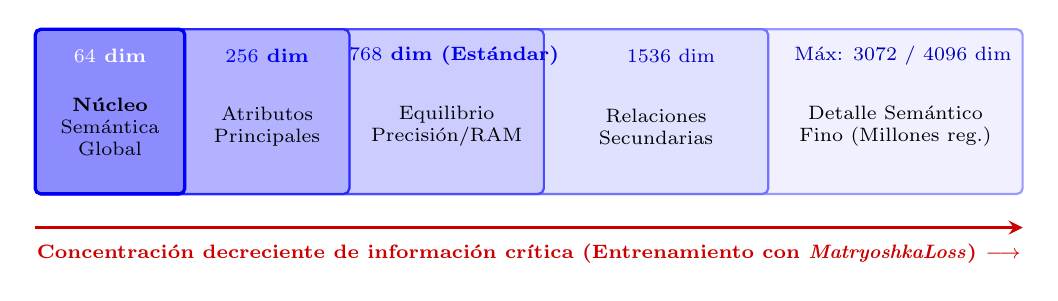
\begin{tikzpicture}[scale=0.95]
% Cajas anidadas Matryoshka
\draw[fill=blue!6, draw=blue!40, thick, rounded corners=2pt] (0,0) rectangle (13.2, 2.2);
\node[font=\scriptsize, blue!70!black] at (11.6, 1.85) {Máx: $3072$ / $4096$ dim};

\draw[fill=blue!12, draw=blue!55, thick, rounded corners=2pt] (0,0) rectangle (9.8, 2.2);
\node[font=\scriptsize, blue!80!black] at (8.5, 1.85) {$1536$ dim};

\draw[fill=blue!20, draw=blue!70, thick, rounded corners=2pt] (0,0) rectangle (6.8, 2.2);
\node[font=\scriptsize\bfseries, blue!90!black] at (5.6, 1.85) {$768$ dim (Estándar)};

\draw[fill=blue!30, draw=blue!85, thick, rounded corners=2pt] (0,0) rectangle (4.2, 2.2);
\node[font=\scriptsize\bfseries, blue!95!black] at (3.1, 1.85) {$256$ dim};

\draw[fill=blue!45, draw=blue!95!black, very thick, rounded corners=2pt] (0,0) rectangle (2.0, 2.2);
\node[font=\scriptsize\bfseries, white] at (1.0, 1.85) {$64$ dim};

% Etiquetas inferiores de densidad de información
\node[font=\scriptsize, align=center] at (1.0, 0.9) {\textbf{Núcleo}\\Semántica\\Global};
\node[font=\scriptsize, align=center] at (3.1, 0.9) {Atributos\\Principales};
\node[font=\scriptsize, align=center] at (5.5, 0.9) {Equilibrio\\Precisión/RAM};
\node[font=\scriptsize, align=center] at (8.3, 0.9) {Relaciones\\Secundarias};
\node[font=\scriptsize, align=center] at (11.5, 0.9) {Detalle Semántico\\Fino (Millones reg.)};

% Flecha de gradiente de importancia
\draw[-stealth, very thick, red!80!black] (0, -0.45) -- (13.2, -0.45);
\node[font=\scriptsize\bfseries, red!80!black] at (6.6, -0.8) {Concentración decreciente de información crítica (Entrenamiento con \textit{MatryoshkaLoss}) $\longrightarrow$};
\end{tikzpicture}
\caption{Estructura jerárquica de un vector entrenado mediante \textit{Matryoshka Representation Learning} (MRL): las primeras dimensiones concentran la mayor carga semántica, permitiendo truncar el vector de salida para reducir exponencialmente el consumo de memoria RAM y latencia con penalizaciones mínimas de precisión \cite{learnopencv_qwen3, gemini_emb2_docs}.}
\label{fig:matryoshka_mrl}
\end{figure}

Ahora bien, desde el punto de vista de la implementación algorítmica rigurosa, truncar un vector unitario $\mathbf{v} \in \mathbb{R}^{D}$ (donde $\|\mathbf{v}\|_2 = 1$) a sus primeras $d < D$ componentes ($\mathbf{v}_{1:d}$) hace que la suma de cuadrados de las coordenadas retenidas sea estrictamente menor que la unidad ($\sum_{j=1}^{d} v_j^2 < 1$). Dado que los vectores truncados (por ejemplo, al configurar $d = 768$ o $d = 1536$ en lugar de las $3072$ dimensiones completas en \textit{Gemini Embedding 2}) no vienen normalizados de fábrica tras el corte, resulta obligatorio aplicar una etapa explícita de \textbf{re-normalización mediante la norma euclídea $L_2$} según se define en la Ecuación~\eqref{eq:renormalizacion_l2_mrl} antes de insertarlos en la base de datos vectorial \cite{gemini_emb2_docs}:

\begin{equation}
\hat{\mathbf{v}}_{1:d} = \frac{\mathbf{v}_{1:d}}{\|\mathbf{v}_{1:d}\|_2} = \frac{(v_1, v_2, \dots, v_d)^\top}{\sqrt{\sum_{j=1}^{d} v_j^2}}
\label{eq:renormalizacion_l2_mrl}
\end{equation}

Esta operación proyecta de nuevo el sub-vector truncado sobre la superficie de la hipersfera unitaria de dimensión $d$, garantizando que las búsquedas posteriores por Similitud del Coseno en motores como Qdrant mantengan su consistencia matemática y velocidad de cómputo.

\subsubsection{Análisis del Compromiso entre Precisión Semántica y Coste de Almacenamiento}
\label{subsubsec:compromiso_precision_almacenamiento}

La elección de la dimensionalidad operativa del espacio latente introduce un compromiso directo (\textit{trade-off}) de arquitectura entre la granularidad de discriminación semántica y los costes de infraestructura \cite{gemini_emb2_docs, qwen3_vl_emb2026}. Como se sintetiza en el Cuadro~\ref{tab:compromiso_dimensiones}, trabajar con el espacio completo de \textbf{3.072 dimensiones} en \textit{Gemini Embedding 2} (o \textbf{4.096 dimensiones} en \textit{Qwen3-VL-Embedding-8B}) permite capturar un nivel de detalle semántico superior, lo cual resulta determinante cuando la base de datos acumula millones de registros multimodales y se requiere evitar falsos positivos ante consultas altamente específicas \cite{gemini_emb2_docs, qwen3_vl_emb2026}.

\begin{table}[htbp]
\centering
\small
\setlength{\tabcolsep}{4.5pt}
\caption{Comparativa técnica del impacto de la dimensionalidad vectorial y el soporte MRL sobre la precisión semántica y el coste de almacenamiento en bases de datos vectoriales \cite{gemini_emb2_docs, qwen3_vl_emb2026}.}
\label{tab:compromiso_dimensiones}
\begin{tabularx}{\linewidth}{>{\raggedright\arraybackslash}p{2.7cm} >{\raggedright\arraybackslash}p{3.3cm} >{\centering\arraybackslash}p{1.6cm} >{\centering\arraybackslash}p{1.7cm} >{\raggedright\arraybackslash}X}
\toprule
\textbf{Configuración} & \textbf{Modelos de Referencia} & \textbf{Peso (FP32)} & \textbf{Norm. $L_2$} & \textbf{Caso de Uso Óptimo} \\
\midrule
4.096 dim (Máx. Open) & Qwen3-VL-Embedding-8B & 16,0 KB & Nativa & Máxima resolución en servidor GPU local \\
3.072 dim (Máx. Cloud) & Gemini Embedding 2 & 12,0 KB & Nativa & \textit{Baseline} de máxima precisión y millones de reg. \\
2.048 dim (Intermedia) & Qwen3-VL-Embedding-2B & 8,0 KB & Nativa / MRL & Despliegue local equilibrado en VRAM \\
1.536 dim (MRL Medio) & Gemini Embedding 2 & 6,0 KB & Post-corte & Reducción del 50\% en RAM con alta fidelidad \\
768 dim (Estándar) & Gemini 2 / EmbeddingGemma 2 & 3,0 KB & Post-corte & Ahorro del 75\% en BD y consultas ultrarrápidas \\
64 - 256 dim (Ultraligero) & Qwen3-VL / EmbeddingGemma 2 & 0,25 - 1,0 KB & Post-corte & \textit{Edge computing}, dispositivos móviles y pre-filtrado \\
\bottomrule
\end{tabularx}
\end{table}

Por el contrario, operar sobre un estándar de \textbf{768 dimensiones} (que constituye el tope nativo de modelos ligeros modulares como \textit{EmbeddingGemma 2} (con posibilidad de truncado adicional a $256$ o $128$ dimensiones) y uno de los puntos de corte recomendados en \textit{Gemini Embedding 2}) reduce exactamente en un $75\%$ la huella de memoria de cada vector respecto a las $3.072$ dimensiones (pasando de $12,0\,\text{KB}$ a $3,0\,\text{KB}$ por fragmento en precisión simple de 32 bits). Esta compresión hace que la base de datos vectorial resultante sea significativamente más económica de alojar en memoria RAM y más rápida de consultar localmente, a cambio de asumir una ligera reducción en la granularidad semántica fina frente al vector completo de $3.072$ dimensiones.

\subsubsection{Aprendizaje Contrastivo (\textit{InfoNCE}) y el Fenómeno de la Brecha Modal (\textit{Modality Gap})}
\label{subsubsec:infonce_modality_gap}

Desde el punto de vista de la optimización neuronal, la alineación geométrica entre consultas textuales y fragmentos audiovisuales se entrena mediante funciones objetivo contrastivas simétricas basadas en la pérdida \textbf{\textit{InfoNCE}} (\textit{Noise-Contrastive Estimation}) \cite{vandenoord2018cpc, radford2021clip}. Dado un lote (\textit{mini-batch}) de $B$ pares emparejados $\{(\mathbf{q}_i, \mathbf{v}_i)\}_{i=1}^{B}$ proyectados sobre la hiperesfera unitaria $\mathbb{S}^{d-1}$, el entrenamiento maximiza la similitud de los pares positivos en la diagonal frente a los $B-1$ distractores negativos del lote, modulando la concentración de la distribución mediante un hiperparámetro de temperatura $\tau > 0$:

\begin{equation}
\mathcal{L}_{\text{InfoNCE}} = -\frac{1}{2B} \sum_{i=1}^{B} \left[
\log \frac{\exp\!\left(\text{sim}_{\cos}(\mathbf{q}_i, \mathbf{v}_i) / \tau\right)}{\sum_{j=1}^{B} \exp\!\left(\text{sim}_{\cos}(\mathbf{q}_i, \mathbf{v}_j) / \tau\right)} +
\log \frac{\exp\!\left(\text{sim}_{\cos}(\mathbf{v}_i, \mathbf{q}_i) / \tau\right)}{\sum_{j=1}^{B} \exp\!\left(\text{sim}_{\cos}(\mathbf{v}_i, \mathbf{q}_j) / \tau\right)}
\right]
\label{eq:infonce_loss}
\end{equation}

En la Ecuación~\eqref{eq:infonce_loss}, la temperatura $\tau$ controla la severidad con la que se penalizan los ejemplos negativos cercanos. Sin embargo, Liang et al. \cite{liang2022modalitygap} demostraron un fenómeno topológico inherente a los espacios contrastivos multimodales denominado \textbf{\textit{Modality Gap} (Brecha Modal)}: debido a que los codificadores de distinta modalidad nacen en regiones cónicas disjuntas de $\mathbb{S}^{d-1}$ tras la inicialización aleatoria, y a que la pérdida InfoNCE depende exclusivamente de las \textit{diferencias relativas} entre los pares positivos y negativos escaladas por $1/\tau$, la optimización converge preservando un desplazamiento vectorial sistemático entre el subespacio textual y el subespacio visual/audiovisual.

Esta propiedad explica rigurosamente un hallazgo empírico central observado en la literatura y en nuestros experimentos sobre \textit{Gemini Embedding 2} y \textit{Qwen3-VL-Embedding}: incluso cuando un par consulta-fragmento constituye un acierto semántico inequívoco de rango \#1, su similitud del coseno cruzada (\textit{cross-modal}) rara vez se aproxima a $1,0$, agrupándose de manera natural dentro de la banda $[0{,}28;\, 0{,}50]$ (mientras que pares intramodales texto-texto alcanzan valores mucho mayores). En consecuencia, el \textit{Modality Gap} invalida cualquier mecanismo de filtrado basado en umbrales fijos de coseno en la Etapa 1 y fundamenta la necesidad teórica de delegar la discriminación definitiva y el rechazo de falsos positivos a un verificador bimodal de Etapa 2.
\newpage

% Bloque 2.2: Funcionamiento y Taxonomía de Modelos de Embeddings (Págs. 6-10)
% =============================================================================
% CAPÍTULO 2 - BLOQUE 2.2: FUNCIONAMIENTO Y TAXONOMÍA DE MODELOS DE EMBEDDINGS:
% DE LA ALINEACIÓN PROYECTADA A LAS TOPOLOGÍAS ASIMÉTRICAS BI/CROSS-ENCODER
% =============================================================================

\subsection{Funcionamiento y Taxonomía de Modelos de Embeddings Multimodales}
\label{subsec:taxonomia_modelos}

\subsubsection{Evolución Arquitectónica: De los Modelos Alineados (CLIP e ImageBind) a la Omnimodalidad Nativa}
\label{subsubsec:evolucion_clip_omnimodalidad}

El diseño de redes neuronales capaces de proyectar múltiples modalidades de datos dentro de un espacio métrico común ha atravesado tres generaciones claramente diferenciadas en la literatura científica reciente \cite{prajwal2025multimodal, qwen3_vl_emb2026}. Comprender las limitaciones estructurales de las dos primeras generaciones resulta indispensable para justificar la adopción de los modelos fundacionales omnimodales desarrollados entre finales de 2024 y 2026 \cite{gemini_emb2_docs, qwen3_vl_emb2026}.

Durante la primera etapa evolutiva, el estándar de la industria estuvo dominado por modelos de alineación dual o múltiple como \textbf{CLIP} (\textit{Contrastive Language-Image Pre-training}, desarrollado por OpenAI) e \textbf{ImageBind} (desarrollado por Meta) \cite{prajwal2025multimodal}. Estas arquitecturas lograron un hito fundacional al demostrar que era posible entrenar codificadores separados (un codificador visual y un codificador textual) mediante aprendizaje contrastivo para alinear texto e imágenes estáticas (y, en casos puntuales como ImageBind, señales de audio) dentro de un mismo hiperplano vectorial \cite{prajwal2025multimodal}. Sin embargo, cuando estas arquitecturas de primera generación se aplicaban a la recuperación de información en secuencias de vídeo de larga duración, presentaban una limitación insalvable: carecían de una comprensión temporal nativa e integrada \cite{prajwal2025multimodal, rethinking_long_video2026}. Como consecuencia, la arquitectura tradicional obligaba a descomponer artificialmente el flujo multimedia: los ingenieros debían extraer y procesar los fotogramas de manera aislada, emplear modelos de transcripción fonética independientes para la pista de audio (como Whisper) y terminar indexando toda la información resultante como texto plano \cite{video_rag2024}. Este flujo fragmentado no solo resultaba computacionalmente torpe, sino que destruía el contexto temporal y la sincronía entre la acción visual y el suceso acústico \cite{prajwal2025multimodal}.

Una segunda generación de transición surgió a principios de 2025 con propuestas académicas como \textbf{VLM2Vec} y arquitecturas de interacción tardía como \textbf{ColQwen} \cite{prajwal2025multimodal}. El mérito científico de \textit{VLM2Vec} (construido sobre modelos de lenguaje visuales genéricos como LLaVA y Phi) consistió en demostrar empíricamente cómo transformar un Modelo de Lenguaje Visual (\textit{Vision-Language Model}, VLM) originalmente concebido para la generación autorregresiva de texto en un extractor masivo de \textit{embeddings} multimodales para texto, imagen y vídeo. En paralelo, sistemas como \textit{ColQwen} demostraron que era posible eliminar los motores OCR intermedios proyectando directamente las teselas visuales hacia el espacio latente del lenguaje \cite{prajwal2025multimodal}.

Finalmente, entre finales de 2024 y el primer trimestre de 2026 se consolida la tercera generación: los \textbf{Modelos de Embedding Omnimodales (\textit{Omni-modality})} \cite{gemini_emb2_docs, qwen3_vl_emb2026}. Liderados en el ámbito comercial por \textbf{Gemini Embedding 2} (Google) y en el ecosistema de pesos abiertos por la familia \textbf{Qwen3-VL-Embedding} (Alibaba) y \textbf{EmbeddingGemma 2} (Google DeepMind), estos sistemas han sido diseñados desde su pre-entrenamiento para ingerir de forma nativa texto, imágenes, secuencias de vídeo, pistas de audio y documentos estructurados (archivos PDF) proyectándolos directamente en un único vector denso sin pasos de traducción textual intermedios \cite{gemini_emb2_docs, qwen3_vl_emb2026}.

La Figura~\ref{fig:evolucion_generaciones_embeddings} sintetiza gráficamente la transición arquitectónica a través de estas tres generaciones de modelos de representación.

\begin{figure}[htbp]
\centering
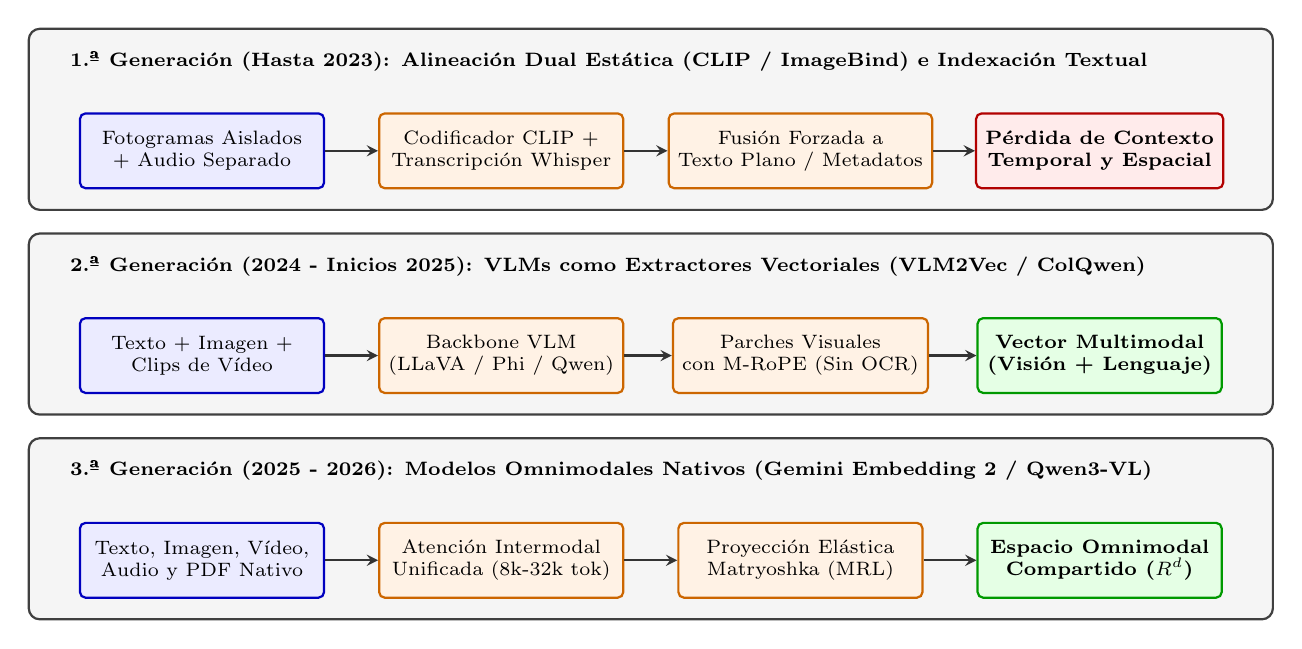
\begin{tikzpicture}[
    node distance=0.5cm and 0.6cm,
    genbox/.style={rectangle, draw=black!75, fill=gray!8, thick, minimum width=15.8cm, minimum height=2.3cm, rounded corners=4pt},
    modbox/.style={rectangle, draw=blue!75!black, fill=blue!8, thick, minimum width=3.1cm, minimum height=0.95cm, align=center, font=\scriptsize, rounded corners=2pt},
    procbox/.style={rectangle, draw=orange!80!black, fill=orange!10, thick, minimum width=3.1cm, minimum height=0.95cm, align=center, font=\scriptsize, rounded corners=2pt},
    outbox/.style={rectangle, draw=green!60!black, fill=green!10, thick, minimum width=3.1cm, minimum height=0.95cm, align=center, font=\scriptsize\bfseries, rounded corners=2pt},
    arrow/.style={-stealth, thick, draw=black!80}
]
% Generación 1
\node[genbox] (g1) at (0, 5.2) {};
\node[font=\scriptsize\bfseries, anchor=north west] at (-7.5, 6.18) {1.ª Generación (Hasta 2023): Alineación Dual Estática (CLIP / ImageBind) e Indexación Textual};
\node[modbox] (g1_in) at (-5.7, 4.80) {Fotogramas Aislados\\+ Audio Separado};
\node[procbox] (g1_proc) at (-1.9, 4.80) {Codificador CLIP +\\Transcripción Whisper};
\node[procbox] (g1_txt) at (1.9, 4.80) {Fusión Forzada a\\Texto Plano / Metadatos};
\node[outbox, draw=red!70!black, fill=red!8] (g1_out) at (5.7, 4.80) {Pérdida de Contexto\\Temporal y Espacial};
\draw[arrow] (g1_in) -- (g1_proc);
\draw[arrow] (g1_proc) -- (g1_txt);
\draw[arrow] (g1_txt) -- (g1_out);

% Generación 2
\node[genbox] (g2) at (0, 2.6) {};
\node[font=\scriptsize\bfseries, anchor=north west] at (-7.5, 3.58) {2.ª Generación (2024 - Inicios 2025): VLMs como Extractores Vectoriales (VLM2Vec / ColQwen)};
\node[modbox] (g2_in) at (-5.7, 2.20) {Texto + Imagen +\\Clips de Vídeo};
\node[procbox] (g2_proc) at (-1.9, 2.20) {Backbone VLM\\(LLaVA / Phi / Qwen)};
\node[procbox] (g2_mrope) at (1.9, 2.20) {Parches Visuales\\con M-RoPE (Sin OCR)};
\node[outbox] (g2_out) at (5.7, 2.20) {Vector Multimodal\\(Visión + Lenguaje)};
\draw[arrow] (g2_in) -- (g2_proc);
\draw[arrow] (g2_proc) -- (g2_mrope);
\draw[arrow] (g2_mrope) -- (g2_out);

% Generación 3
\node[genbox] (g3) at (0, 0.0) {};
\node[font=\scriptsize\bfseries, anchor=north west] at (-7.5, 0.98) {3.ª Generación (2025 - 2026): Modelos Omnimodales Nativos (Gemini Embedding 2 / Qwen3-VL)};
\node[modbox] (g3_in) at (-5.7, -0.40) {Texto, Imagen, Vídeo,\\Audio y PDF Nativo};
\node[procbox] (g3_proc) at (-1.9, -0.40) {Atención Intermodal\\Unificada (8k-32k tok)};
\node[procbox] (g3_mrl) at (1.9, -0.40) {Proyección Elástica\\Matryoshka (MRL)};
\node[outbox] (g3_out) at (5.7, -0.40) {Espacio Omnimodal\\Compartido ($\mathbb{R}^d$)};
\draw[arrow] (g3_in) -- (g3_proc);
\draw[arrow] (g3_proc) -- (g3_mrl);
\draw[arrow] (g3_mrl) -- (g3_out);
\end{tikzpicture}
\caption{Evolución taxonómica de los modelos de representación vectorial: desde la alineación estática dependiente de transcripción textual (CLIP/Whisper) hasta los modelos omnimodales nativos de tercera generación capaces de proyectar texto, imagen, vídeo, audio y PDF en un único clúster topológico \cite{prajwal2025multimodal, gemini_emb2_docs, qwen3_vl_emb2026}.}
\label{fig:evolucion_generaciones_embeddings}
\end{figure}

\subsubsection{Tokenización Visual, Codificación M-RoPE y Agregación Temporal de Fotogramas}
\label{subsubsec:tokenizacion_mrope_agregacion}

A nivel interno, el funcionamiento de un modelo de \textit{embedding} multimodal contemporáneo se apoya en la unificación de la representación de entrada mediante teselas o parches (\textit{visual patches}) procesados por arquitecturas inspiradas en \textit{Vision Transformers} (ViT) \cite{prajwal2025multimodal}. Cuando el sistema recibe un fotograma de vídeo o una página de un documento visual a su resolución nativa, divide la matriz bidimensional de píxeles en una secuencia de sub-bloques que se proyectan linealmente como \textit{tokens} visuales dentro de la misma secuencia de entrada que los \textit{tokens} léxicos del texto \cite{prajwal2025multimodal}.

Para evitar que esta linealización destruya la geometría bidimensional de la imagen o la secuencia temporal del vídeo, las arquitecturas modernas incorporan \textbf{\textit{Multimodal Rotary Position Embeddings}} (\textbf{M-RoPE}) \cite{prajwal2025multimodal}. M-RoPE codifica directamente la información posicional bidimensional y temporal sobre las representaciones latentes de cada parche visual, lo que resulta determinante al procesar fotogramas de vídeo con resoluciones variables, garantizando que las relaciones espaciales entre los objetos visuales (como un bloque de código fuente en una esquina de la pantalla y el ponente en el lado opuesto) queden alineadas en el mismo espacio vectorial que los \textit{tokens} del Modelo de Lenguaje Grande (LLM) subyacente \cite{prajwal2025multimodal}.

Un aspecto arquitectónico fundamental en la vectorización de fragmentos de vídeo (\texttt{VideoChunk}) radica en el mecanismo de \textbf{agregación temporal de múltiples fotogramas} \cite{gemini_emb2_docs}. Cuando un algoritmo de segmentación semántica adaptativa (como \textit{Video-RAC}) extrae tres fotogramas representativos de un plano (el fotograma inicial, el de máxima entropía visual y el fotograma final), existen dos formas opuestas de invocar al modelo fundacional \cite{video_rac2025, gemini_emb2_docs}:
\begin{enumerate}
    \item \textbf{Codificación Independiente por Fotograma (Incorrecta para cohesión de \textit{chunk}):} Si los tres fotogramas se envían a la API como tres objetos de contenido separados, el modelo genera tres vectores independientes ($\mathbf{v}_1, \mathbf{v}_2, \mathbf{v}_3 \in \mathbb{R}^d$). Esto triplica el coste de almacenamiento en la base de datos vectorial y obliga a realizar promedios heurísticos posteriores que diluyen la semántica temporal del plano.
    \item \textbf{Agregación Nativa en un Único Objeto \texttt{Content} (Estado del Arte):} En arquitecturas como \textit{Gemini Embedding 2}, al codificar los tres fotogramas clave en memoria (por ejemplo, en formato JPEG) e inyectarlos como múltiples objetos \texttt{Part} dentro de una única estructura \texttt{types.Content}, el mecanismo de atención interna del modelo evalúa conjuntamente la evolución entre los tres instantes y devuelve \textbf{un único \textit{embedding} denso agregado} $\mathbf{v}_{\text{chunk}} \in \mathbb{R}^d$ que sintetiza el significado completo del evento \cite{gemini_emb2_docs}.
\end{enumerate}

La Figura~\ref{fig:agregacion_temporal_content} ilustra cómo la agrupación de múltiples partes multimedia dentro de un mismo contenedor \texttt{Content} permite condensar la dinámica del fragmento temporal en un único punto del espacio latente.

\begin{figure}[htbp]
\centering
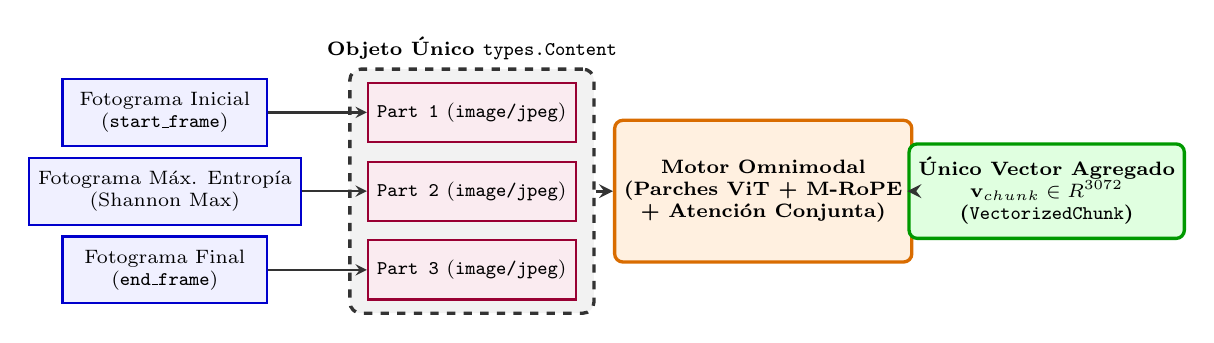
\begin{tikzpicture}[
    node distance=0.6cm and 0.8cm,
    framebox/.style={rectangle, draw=blue!80!black, fill=blue!6, thick, minimum width=2.6cm, minimum height=0.85cm, align=center, font=\scriptsize},
    partbox/.style={rectangle, draw=purple!80!black, fill=purple!8, thick, minimum width=2.4cm, minimum height=0.75cm, align=center, font=\scriptsize},
    contentbox/.style={rectangle, draw=black!80, fill=gray!10, very thick, dashed, minimum width=3.1cm, minimum height=3.1cm, rounded corners=4pt},
    modelbox/.style={rectangle, draw=orange!85!black, fill=orange!12, very thick, minimum width=3.0cm, minimum height=1.8cm, align=center, font=\scriptsize\bfseries, rounded corners=3pt},
    vecbox/.style={rectangle, draw=green!60!black, fill=green!12, very thick, minimum width=3.0cm, minimum height=1.2cm, align=center, font=\scriptsize\bfseries, rounded corners=3pt},
    arrow/.style={-stealth, thick, draw=black!80}
]
% Fotogramas extraídos del VideoChunk
\node[framebox] (f1) at (-5.2, 1.0) {Fotograma Inicial\\(\texttt{start\_frame})};
\node[framebox] (f2) at (-5.2, 0.0) {Fotograma Máx. Entropía\\(Shannon Max)};
\node[framebox] (f3) at (-5.2, -1.0) {Fotograma Final\\(\texttt{end\_frame})};

% Contenedor único types.Content
\node[contentbox] (cont) at (-1.3, 0.0) {};
\node[font=\scriptsize\bfseries, anchor=south] at (-1.3, 1.55) {Objeto Único \texttt{types.Content}};
\node[partbox] (p1) at (-1.3, 1.0) {\texttt{Part 1} (\texttt{image/jpeg})};
\node[partbox] (p2) at (-1.3, 0.0) {\texttt{Part 2} (\texttt{image/jpeg})};
\node[partbox] (p3) at (-1.3, -1.0) {\texttt{Part 3} (\texttt{image/jpeg})};

% Modelo y salida
\node[modelbox] (mod) at (2.4, 0.0) {Motor Omnimodal\\(Parches ViT + M-RoPE\\+ Atención Conjunta)};
\node[vecbox] (vec) at (6.0, 0.0) {Único Vector Agregado\\$\mathbf{v}_{\text{chunk}} \in \mathbb{R}^{3072}$\\(\texttt{VectorizedChunk})};

\draw[arrow] (f1) -- (p1);
\draw[arrow] (f2) -- (p2);
\draw[arrow] (f3) -- (p3);
\draw[arrow, very thick] (cont.east) -- (mod.west);
\draw[arrow, very thick] (mod.east) -- (vec.west);
\end{tikzpicture}
\caption{Mecanismo de agregación intermodal en \textit{Gemini Embedding 2}: los tres fotogramas representativos de un \texttt{VideoChunk} se empaquetan como objetos \texttt{Part} individuales dentro de un único contenedor \texttt{types.Content}, permitiendo que el modelo fusione la información temporal y devuelva un único vector denso por fragmento \cite{gemini_emb2_docs, video_rac2025}.}
\label{fig:agregacion_temporal_content}
\end{figure}

\subsubsection{Arquitecturas de Doble Torre (\textit{Bi-Encoder}) para Recuperación Masiva Pre-computada}
\label{subsubsec:arquitectura_bi_encoder}

En el diseño de sistemas de recuperación de información sobre grandes volúmenes de vídeo, la primera etapa del procesamiento recae sobre los modelos con \textbf{arquitectura de Doble Torre (\textit{Bi-Encoder})}, representados en el estado del arte por sistemas como \textit{Gemini Embedding 2}, \textit{Qwen3-VL-Embedding} (en sus variantes de 2B y 8B de parámetros) y \textit{EmbeddingGemma 2} \cite{gemini_emb2_docs, qwen3_vl_emb2026}.

La característica definitoria de un \textit{Bi-Encoder} es que procesa de manera completamente independiente el documento multimedia candidato $D_i$ (un fragmento de vídeo, una imagen o una pista de audio) y la consulta textual del usuario $Q$ \cite{learnopencv_qwen3, qwen3_vl_emb2026}. Matemáticamente, sean $f_{\theta}^{\text{doc}}$ y $f_{\theta}^{\text{query}}$ las funciones de proyección de ambas torres (que en los modelos fundacionales modernos suelen compartir los mismos pesos neuronales $\theta$, diferenciándose únicamente por el prefijo de instrucción de entrada), según se define en la Ecuación~\eqref{eq:bi_encoder_proyeccion} \cite{hf_train_multimodal2026}:

\begin{equation}
\mathbf{v}_i = f_{\theta}^{\text{doc}}(D_i) \in \mathbb{R}^d, \qquad \mathbf{q} = f_{\theta}^{\text{query}}(P_{\text{task}} \oplus Q) \in \mathbb{R}^d
\label{eq:bi_encoder_proyeccion}
\end{equation}

donde $P_{\text{task}}$ representa un prefijo corto de instrucción de tarea que se antepone exclusivamente a las entradas de texto para orientar la consulta en el espacio latente (técnica empleada explícitamente en modelos como \textit{EmbeddingGemma 2} y \textit{Qwen3-VL-Embedding}, pero que no se aplica a las imágenes, vídeos ni audios) \cite{qwen3_vl_emb2026}.

Esta independencia algebraica entre $\mathbf{v}_i$ y $\mathbf{q}$ constituye la piedra angular de la escalabilidad industrial por tres motivos fundamentales \cite{learnopencv_qwen3}:
\begin{enumerate}
    \item \textbf{Indexación Pasiva \textit{Offline}:} Permite pre-computar una sola vez los vectores $\mathbf{v}_i$ de un archivo histórico compuesto por millones de horas de vídeo y almacenarlos pasivamente en bases de datos vectoriales indexadas estáticamente como Qdrant o Milvus \cite{learnopencv_qwen3}.
    \item \textbf{Complejidad de Inferencia Constante respecto al Modelo:} Cuando el usuario introduce una búsqueda en lenguaje natural en tiempo de ejecución, la red neuronal profunda solo se ejecuta una vez para codificar la consulta $\mathbf{q}$ \cite{learnopencv_qwen3}.
    \item \textbf{Maximización de la Tasa de Recuerdo (\textit{Recall}) a Escala de Petabytes:} La recuperación se reduce a comparar el vector $\mathbf{q}$ recién generado contra los millones de vectores pre-computados mediante operaciones vectoriales ultrarrápidas (como el producto punto escalar o la similitud del coseno), logrando tiempos de respuesta de milisegundos \cite{learnopencv_qwen3, qwen3_vl_emb2026}.
\end{enumerate}

\subsubsection{Arquitecturas de Torre Única (\textit{Cross-Encoder / Reranker}) y Atención Cruzada}
\label{subsubsec:arquitectura_cross_encoder}

A pesar de su extraordinaria velocidad, los modelos \textit{Bi-Encoder} sufren una limitación estructural derivada de comprimir todo un fragmento de vídeo en un único vector estático $\mathbf{v}_i$ sin conocer de antemano qué preguntará el usuario \cite{learnopencv_qwen3, qwen3_vl_emb2026}. Al no existir interacción directa entre los \textit{tokens} de la consulta y los parches visuales del vídeo durante la codificación, ciertos detalles composicionales finos o textos pequeños en pantalla pueden quedar diluidos dentro de la representación global.

Para resolver esta pérdida de precisión sin sacrificar la escalabilidad, el estado del arte introduce los modelos con \textbf{arquitectura de Torre Única (\textit{Cross-Encoder})}, denominados operativamente \textbf{\textit{Rerankers}} (reordenadores) o verificadores visuales de segunda etapa, entre los que destacan \textbf{Qwen3-VL-Reranker} (en variantes de 2B y 8B) y el uso de modelos ligeros de visión-lenguaje como \textbf{Gemini 1.5 Flash Lite} o \textbf{Gemini Flash 3.5} en tareas de validación visual \cite{learnopencv_qwen3, qwen3_vl_emb2026}.

A diferencia del \textit{Bi-Encoder}, un \textit{Cross-Encoder} no genera vectores independientes ni permite pre-computar representaciones de los vídeos \cite{learnopencv_qwen3}. En su lugar, recibe simultáneamente en una única secuencia concatenada la consulta del usuario $Q$ y el fragmento multimedia candidato $D_k$, procesándolos conjuntamente a través de todas las capas de \textbf{Atención Cruzada (\textit{Cross-Attention})} del \textit{Transformer}, como se formula en la Ecuación~\eqref{eq:cross_encoder_score} \cite{learnopencv_qwen3, qwen3_vl_emb2026}:

\begin{equation}
s_k = g_{\phi}(Q, D_k) = \sigma\!\left(\mathbf{W}_{\text{head}} \cdot \text{CrossAttention}_{\phi}\!\left([\text{Tokens}(Q); \, \text{Patches}(D_k)]\right)\right) \in [0, 1]
\label{eq:cross_encoder_score}
\end{equation}

Mediante el mecanismo de \textit{Cross-Attention}, cada \textit{token} de la pregunta del usuario (por ejemplo, la palabra \textit{``diccionarios''}) atiende directamente a cada parche visual específico de los fotogramas del candidato $D_k$ (por ejemplo, la región de la pantalla donde aparece escrito el código \texttt{dict \{"name": "Brais"\}}). Finalmente, como refleja el Cuadro de especificaciones de la familia Qwen3-VL, el \textit{Cross-Encoder} no devuelve un vector de \textit{embedding}, sino una \textbf{probabilidad discreta en el rango $[0, 1]$} (o un veredicto de validación visual) que cuantifica la relevancia exacta del candidato respecto a la consulta \cite{qwen3_vl_emb2026}.

La Figura~\ref{fig:bi_encoder_vs_cross_encoder} contrasta detalladamente la topología interna de un \textit{Bi-Encoder} frente a la de un \textit{Cross-Encoder} \cite{learnopencv_qwen3, qwen3_vl_emb2026}.

\begin{figure}[htbp]
\centering
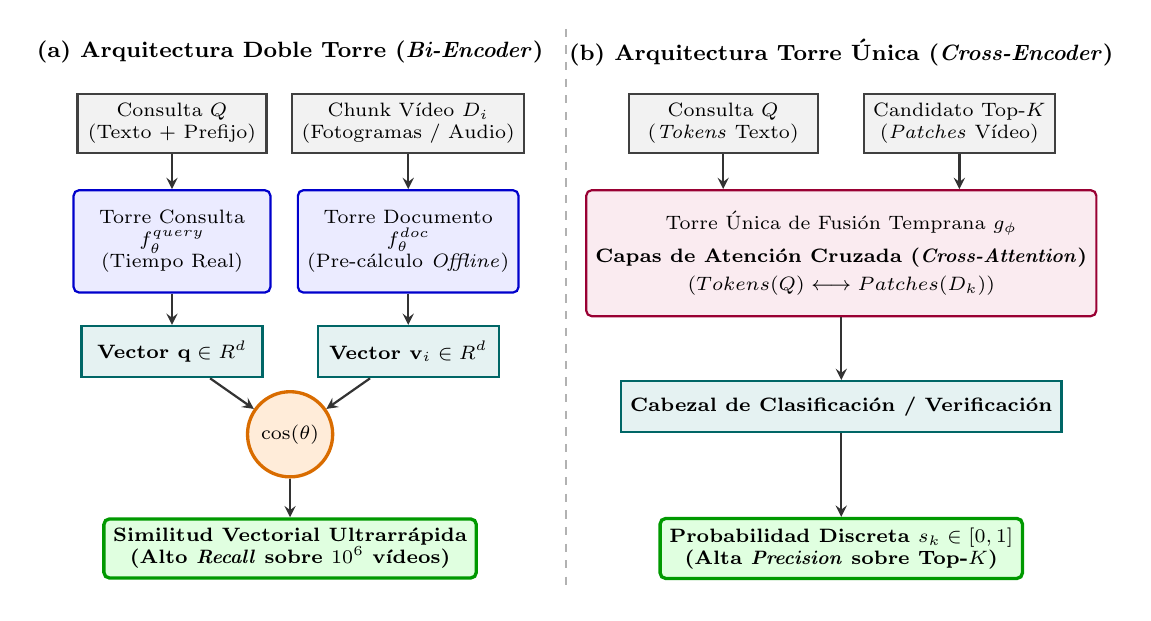
\begin{tikzpicture}[
    node distance=0.5cm and 0.7cm,
    tower/.style={rectangle, draw=blue!80!black, fill=blue!8, thick, minimum width=2.5cm, minimum height=1.3cm, align=center, font=\scriptsize, rounded corners=2pt},
    crosstower/.style={rectangle, draw=purple!80!black, fill=purple!8, thick, minimum width=5.4cm, minimum height=1.6cm, align=center, font=\scriptsize, rounded corners=2pt},
    inputbox/.style={rectangle, draw=black!75, fill=gray!10, thick, minimum width=2.4cm, minimum height=0.75cm, align=center, font=\scriptsize},
    vecnode/.style={rectangle, draw=teal!80!black, fill=teal!10, thick, minimum width=2.3cm, minimum height=0.65cm, align=center, font=\scriptsize\bfseries},
    opnode/.style={circle, draw=orange!85!black, fill=orange!15, very thick, minimum size=0.9cm, align=center, font=\scriptsize\bfseries},
    scorebox/.style={rectangle, draw=green!60!black, fill=green!12, very thick, minimum width=3.2cm, minimum height=0.75cm, align=center, font=\scriptsize\bfseries, rounded corners=2pt},
    arrow/.style={-stealth, thick, draw=black!80}
]
% --- LADO IZQUIERDO: BI-ENCODER ---
\node[font=\bfseries\footnotesize] at (-3.5, 4.0) {(a) Arquitectura Doble Torre (\textit{Bi-Encoder})};

\node[inputbox] (bi_q) at (-5.0, 3.1) {Consulta $Q$\\(Texto + Prefijo)};
\node[inputbox] (bi_d) at (-2.0, 3.1) {Chunk Vídeo $D_i$\\(Fotogramas / Audio)};

\node[tower] (t_q) at (-5.0, 1.6) {Torre Consulta\\$f_{\theta}^{\text{query}}$\\(Tiempo Real)};
\node[tower] (t_d) at (-2.0, 1.6) {Torre Documento\\$f_{\theta}^{\text{doc}}$\\(Pre-cálculo \textit{Offline})};

\node[vecnode] (v_q) at (-5.0, 0.2) {Vector $\mathbf{q} \in \mathbb{R}^d$};
\node[vecnode] (v_d) at (-2.0, 0.2) {Vector $\mathbf{v}_i \in \mathbb{R}^d$};

\node[opnode] (cos) at (-3.5, -0.85) {$\cos(\theta)$};
\node[scorebox] (bi_out) at (-3.5, -2.30) {Similitud Vectorial Ultrarrápida\\(Alto \textit{Recall} sobre $10^6$ vídeos)};

\draw[arrow] (bi_q) -- (t_q);
\draw[arrow] (bi_d) -- (t_d);
\draw[arrow] (t_q) -- (v_q);
\draw[arrow] (t_d) -- (v_d);
\draw[arrow] (v_q) -- (cos);
\draw[arrow] (v_d) -- (cos);
\draw[arrow] (cos) -- (bi_out);

% Línea divisoria central
\draw[dashed, gray!60, thick] (0.0, 4.3) -- (0.0, -2.85);

% --- LADO DERECHO: CROSS-ENCODER ---
\node[font=\bfseries\footnotesize] at (3.5, 4.0) {(b) Arquitectura Torre Única (\textit{Cross-Encoder})};

\node[inputbox] (cr_q) at (2.0, 3.1) {Consulta $Q$\\(\textit{Tokens} Texto)};
\node[inputbox] (cr_d) at (5.0, 3.1) {Candidato Top-$K$\\(\textit{Patches} Vídeo)};

\node[crosstower] (cr_t) at (3.5, 1.45) {Torre Única de Fusión Temprana $g_{\phi}$\\[4pt]
\textbf{Capas de Atención Cruzada (\textit{Cross-Attention})}\\[2pt]
($\text{Tokens}(Q) \longleftrightarrow \text{Patches}(D_k)$)};

\node[vecnode, minimum width=4.2cm] (cr_head) at (3.5, -0.5) {Cabezal de Clasificación / Verificación};
\node[scorebox] (cr_out) at (3.5, -2.30) {Probabilidad Discreta $s_k \in [0, 1]$\\(Alta \textit{Precision} sobre Top-$K$)};

\draw[arrow] (cr_q) -- (cr_q |- cr_t.north);
\draw[arrow] (cr_d) -- (cr_d |- cr_t.north);
\draw[arrow] (cr_t) -- (cr_head);
\draw[arrow] (cr_head) -- (cr_out);
\end{tikzpicture}
\caption{Comparativa estructural entre (a) un \textit{Bi-Encoder} de doble torre que codifica consulta y vídeo de forma independiente para indexación pasiva en bases de datos vectoriales, y (b) un \textit{Cross-Encoder} (\textit{Reranker}) que aplica atención cruzada conjunta sobre el subconjunto de candidatos recuperados \cite{learnopencv_qwen3, qwen3_vl_emb2026}.}
\label{fig:bi_encoder_vs_cross_encoder}
\end{figure}

\subsubsection{Eficiencia Escalable: El Paradigma de Búsqueda Asimétrica en Dos Etapas (Regla 99\% / 1\%)}
\label{subsubsec:busqueda_asimetrica_dos_etapas}

El resurgimiento y perfeccionamiento de la dualidad entre \textit{Bi-Encoders} (para recuperación inicial) y \textit{Cross-Encoders} o verificadores VLM (para refinamiento) responde directamente a los límites físicos de energía, latencia y procesamiento de hardware en sistemas de vídeo a gran escala \cite{learnopencv_qwen3, rethinking_long_video2026}. Computar de forma cruzada cada búsqueda del usuario contra terabytes de fragmentos de vídeo utilizando modelos generativos masivos (como intentar emplear un modelo tipo Llama-Vision o Gemini Pro para comparar fotograma a fotograma todo un repositorio) resulta técnica y financieramente inasumible \cite{learnopencv_qwen3}.

Para resolver esta dicotomía, el estado del arte de 2026 establece una \textbf{aproximación asimétrica radical en dos etapas} conocida como la regla del $99\% / 1\%$ \cite{learnopencv_qwen3, qwen3_vl_emb2026}:
\begin{itemize}
    \item \textbf{Primera Etapa - Filtrado Masivo del 99\% (\textit{Bi-Encoder} + Base de Datos Vectorial):} Se delega el $99\%$ del descarte de datos a una vectorización paralela, densa e independiente (empleando modelos como \textit{Gemini Embedding 2} o \textit{Qwen3-VL-Embedding}) almacenada en un motor vectorial como Qdrant \cite{gemini_emb2_docs, qwen3_vl_emb2026}. Ante una consulta del usuario, la búsqueda inicial se resuelve mediante un cálculo vectorial de similitud del coseno sobre índices estáticos, reduciendo instantáneamente miles de fragmentos a una lista acotada de los $K$ mejores candidatos (por ejemplo, $\text{Top-}K = 5$ o $\text{Top-}K = 20$) \cite{learnopencv_qwen3}.
    \item \textbf{Segunda Etapa - Refinamiento Intensivo del 1\% (\textit{Cross-Encoder} / Verificación Visual):} El cómputo pesado, iterativo y apoyado en mecanismos de atención cruzada se reserva exclusivamente para ese $1\%$ de resultados candidatos recuperados en la primera fase \cite{learnopencv_qwen3}. En esta etapa, bien un modelo específico de reordenación (\textit{Qwen3-VL-Reranker}) recalcula la probabilidad exacta de coincidencia $[0, 1]$, o bien un verificador visual ligero (\textit{Gemini 1.5 Flash Lite} / \textit{Gemini Flash 3.5}) inspecciona los fotogramas del \textit{chunk} candidato para descartar falsos positivos antes de presentar los intervalos de tiempo (\texttt{start\_time} - \texttt{end\_time}) definitivos al usuario \cite{learnopencv_qwen3, qwen3_vl_emb2026}.
\end{itemize}

\begin{figure}[htbp]
\centering
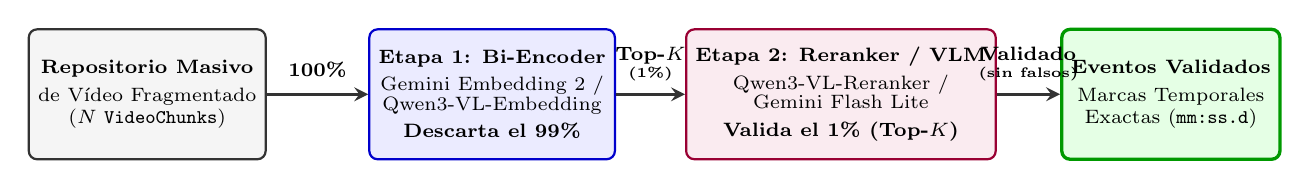
\begin{tikzpicture}[
    node distance=0.5cm and 0.6cm,
    stagebox/.style={rectangle, draw=black!80, fill=gray!8, thick, minimum width=3.0cm, minimum height=1.65cm, align=center, font=\scriptsize, rounded corners=3pt},
    resbox/.style={rectangle, draw=green!60!black, fill=green!10, very thick, minimum width=2.6cm, minimum height=1.65cm, align=center, font=\scriptsize, rounded corners=3pt},
    arrow/.style={-stealth, very thick, draw=black!80}
]
\node[stagebox] (corpus) at (-6.40, 0) {\textbf{Repositorio Masivo}\\[2pt]de Vídeo Fragmentado\\($N$ \texttt{VideoChunks})};

\node[stagebox, draw=blue!80!black, fill=blue!8, minimum width=3.1cm] (etapa1) at (-2.02, 0) {\textbf{Etapa 1: Bi-Encoder}\\[2pt]{\scriptsize Gemini Embedding 2 /}\\[-1pt]{\scriptsize Qwen3-VL-Embedding}\\[2pt]\textbf{Descarta el 99\%}};

\node[stagebox, draw=purple!80!black, fill=purple!8, minimum width=3.1cm] (etapa2) at (2.41, 0) {\textbf{Etapa 2: Reranker / VLM}\\[2pt]{\scriptsize Qwen3-VL-Reranker /}\\[-1pt]{\scriptsize Gemini Flash Lite}\\[2pt]\textbf{Valida el 1\% (Top-$K$)}};

\node[resbox] (final) at (6.60, 0) {\textbf{Eventos Validados}\\[2pt]Marcas Temporales\\Exactas (\texttt{mm:ss.d})};

\draw[arrow] (corpus) -- node[above=2pt, font=\scriptsize\bfseries] {100\%} (etapa1);
\draw[arrow] (etapa1) -- node[above=1pt, font=\scriptsize\bfseries, align=center] {Top-$K$\\[-2pt]{\tiny (1\%)}} (etapa2);
\draw[arrow] (etapa2) -- node[above=1pt, font=\scriptsize\bfseries, align=center] {Validado\\[-2pt]{\tiny (sin falsos)}} (final);
\end{tikzpicture}
\caption{Flujo del paradigma de búsqueda asimétrica en dos etapas (Regla 99\% / 1\%): el \textit{Bi-Encoder} filtra masivamente el repositorio mediante similitud del coseno en Qdrant y el \textit{Cross-Encoder} o verificador visual inspecciona únicamente el subconjunto Top-$K$ para garantizar máxima precisión con latencia mínima \cite{learnopencv_qwen3, qwen3_vl_emb2026}.}
\label{fig:embudo_asimetrico_99_1}
\end{figure}

El Cuadro~\ref{tab:comparativa_bi_cross_verificador} resume las diferencias arquitectónicas, operativas y matemáticas entre las tres familias de modelos que intervienen en el ciclo de recuperación y validación multimodal.

\begin{table}[htbp]
\centering
\small
\caption{Comparativa técnica entre arquitecturas \textit{Bi-Encoder}, \textit{Cross-Encoder} (\textit{Reranker}) y Verificadores VLM Generativos en sistemas Video RAG \cite{learnopencv_qwen3, qwen3_vl_emb2026, gemini_emb2_docs}.}
\label{tab:comparativa_bi_cross_verificador}
\begin{tabularx}{\linewidth}{>{\raggedright\arraybackslash}p{3.2cm}XXX}
\toprule
\textbf{Atributo Técnico} & \textbf{Bi-Encoder (1.ª Etapa)} & \textbf{Cross-Encoder (2.ª Etapa)} & \textbf{Verificador VLM (2.ª Etapa)} \\
\midrule
Modelos de referencia & Gemini Emb. 2 / Qwen3-Emb & Qwen3-VL-Reranker (2B/8B) & Gemini 1.5 Flash Lite / Flash 3.5 \\
Interacción Consulta-Vídeo & Tardía (Producto escalar) & Temprana (\textit{Cross-Attention}) & Generativa multimodal guiada \\
Pre-cálculo \textit{Offline} & Sí (Indexado en Qdrant) & No (Cálculo en tiempo real) & No (Evaluación bajo demanda) \\
Formato de salida & Vector $\mathbf{v} \in \mathbb{R}^d$ (MRL) & Probabilidad discreta $[0, 1]$ & Score + Justificación visual \\
Volumen procesado & $100\%$ corpus (filtra $99\%$) & $1\%$ candidatos (Top-$K$) & $1\%$ candidatos (Top-$K$) \\
Métrica optimizada & Recuerdo (\textit{Recall@K}) & Precisión (\textit{nDCG@K} / \textit{Hit@1}) & Descarte Falsos Positivos \\
\bottomrule
\end{tabularx}
\end{table}

Como demuestra esta taxonomía, la combinación de una primera etapa de vectorización densa omnimodal con una segunda etapa de atención cruzada y verificación visual constituye la arquitectura idónea para localizar eventos específicos en vídeo sin incurrir en costes computacionales prohibitivos \cite{learnopencv_qwen3, qwen3_vl_emb2026}.

% Bloque 2.3: Estudio Profundo de Google Gemini Embedding 2 (Págs. 11-15)
% =============================================================================
% CAPÍTULO 2 - BLOQUE 2.3: ESTUDIO PROFUNDO DE GOOGLE GEMINI EMBEDDING 2:
% ARQUITECTURA OMNIMODAL, MODOS DE INGESTIÓN, MODELADO DE CUOTAS Y RESILIENCIA
% =============================================================================

\subsection{Estudio Profundo de Google Gemini Embedding 2}
\label{subsec:gemini_embedding_2}

\subsubsection{Arquitectura Omnimodal Unificada y Configuración del Espacio de Salida}
\label{subsubsec:arquitectura_gemini_embedding_2}

Dentro de la macrotendencia de modelos fundacionales propietarios accesibles mediante interfaz de programación de aplicaciones (API), \textbf{Gemini Embedding 2} (identificado técnicamente en el catálogo de desarrollo como \texttt{gemini-embedding-2-preview}) constituye el hito arquitectónico de Google hacia la vectorización omnimodal nativa \cite{gemini_emb2_docs, gemini_embeddings_general_docs}. %[cite: 3, 4]
A diferencia de las arquitecturas multimodales de primera generación que requerían codificadores separados y proyecciones post-hoc para cada tipo de dato, \texttt{gemini-embedding-2-preview} ha sido entrenado de extremo a extremo para ingerir texto libre, imágenes estáticas, secuencias de vídeo, pistas de audio y documentos estructurados (archivos PDF) proyectándolos directamente en un único espacio vectorial continuo \cite{gemini_emb2_docs, openrouter_gemini_emb2}. %[cite: 3, 4, 5]

Esta unificación topológica implica que los vectores generados a partir de una consulta textual en lenguaje natural habitan exactamente la misma variedad geométrica que los vectores extraídos de los fotogramas de un vídeo o de una locución hablada \cite{gemini_emb2_docs}. %[cite: 3, 5]
De este modo, la localización de un evento específico dentro de un repositorio audiovisual prescinde por completo de etiquetas manuales previas o de traducciones intermedias a texto plano, resolviéndose mediante el cálculo directo de la similitud del coseno entre la consulta vectorizada y los fragmentos multimedia indexados \cite{gemini_emb2_docs}. %[cite: 3, 5]

En cuanto a la configuración algebraica de sus tensores de salida, el modelo incorpora soporte nativo para \textit{Matryoshka Representation Learning} (MRL) a través del parámetro de configuración \texttt{output\_dimensionality} integrado en la estructura \texttt{types.EmbedContentConfig} del SDK oficial \texttt{google-genai} \cite{gemini_emb2_docs}. %[cite: 3, 4]
Aunque cuando se invoca el punto de enlace sin parámetros adicionales para pruebas básicas de texto el sistema devuelve por defecto un vector compacto de $768$ dimensiones, la arquitectura permite solicitar representaciones de mayor densidad (destacando los estándares operativos de $768$, $1.536$ y el máximo nativo de $3.072$ dimensiones) \cite{gemini_emb2_docs}. %[cite: 3]

Desde la perspectiva de la precisión numérica, existe una distinción crítica en el post-procesamiento de los vectores devueltos por la API según la dimensionalidad seleccionada \cite{gemini_emb2_docs}: %[cite: 3]
\begin{itemize}
    \item \textbf{Operación en Dimensionalidad Máxima ($d = 3.072$):} Los vectores de $3.072$ números en coma flotante devueltos por \texttt{response.embeddings[0].values} se entregan ya normalizados a longitud unitaria por el propio motor de inferencia de Google, ofreciendo la máxima capacidad de discriminación semántica para desambiguar escenas visualmente similares \cite{gemini_emb2_docs}. %[cite: 3]
    \item \textbf{Operación en Dimensionalidades Truncadas ($d < 3.072$):} Cuando el ingeniero configura \texttt{output\_dimensionality} en valores inferiores a $3.072$ (tales como $768$ o $1.536$) con el objetivo de reducir el consumo de memoria en la base de datos vectorial, el recorte de las coordenadas finales altera la magnitud unitaria del vector original \cite{gemini_emb2_docs}. %[cite: 3]
    Por consiguiente, tal y como recomienda la documentación técnica de Google, el cliente de software debe calcular explícitamente la norma euclídea $\|\mathbf{v}\|_2 = \sqrt{\sum_{j=1}^{d} v_j^2}$ (por ejemplo, mediante \texttt{np.linalg.norm(values)}) y dividir cada componente entre dicha norma ($\hat{v}_j = v_j / \|\mathbf{v}\|_2$) siempre que $\|\mathbf{v}\|_2 > 0$, garantizando así la validez geométrica de la similitud del coseno en etapas posteriores \cite{gemini_emb2_docs}. %[cite: 3]
\end{itemize}

\subsubsection{Paradigmas de Ingestión Multimedia en el SDK \texttt{google-genai}: API Files frente a Agregación en Memoria}
\label{subsubsec:paradigmas_ingestion_genai}

La integración programática con el modelo \texttt{gemini-embedding-2-preview} a través de la librería oficial \texttt{google-genai} habilita dos arquitecturas de acoplamiento de datos claramente diferenciadas según la naturaleza del flujo de procesamiento \cite{gemini_emb2_docs, gemini_embeddings_general_docs}: %[cite: 3, 4]

\paragraph{Ingestión de Archivos Completos mediante la API de Almacenamiento Temporal (\texttt{client.files.upload}):}
Orientada al procesamiento directo de ficheros pesados almacenados en disco (clips de vídeo en formato \texttt{video/mp4}, pistas de audio, imágenes de alta resolución o documentos PDF) \cite{gemini_emb2_docs, gemini_embeddings_general_docs}: %[cite: 3]
En este patrón arquitectónico, el sistema no envía los bytes crudos directamente en la llamada de inferencia, sino que ejecuta un protocolo en tres fases \cite{gemini_emb2_docs}: %[cite: 3]
\begin{enumerate}
    \item \textit{Transferencia y generación de URI:} Se invoca el método \texttt{client.files.upload(file=file\_path, config=\{'mime\_type': mime\_type\})}, el cual aloja temporalmente el recurso multimedia en la infraestructura de Google AI Studio y devuelve un objeto con un identificador único (\texttt{uploaded\_file.name}) y una referencia uniforme (\texttt{uploaded\_file.uri}) \cite{gemini_emb2_docs}. %[cite: 3]
    \item \textit{Bucle de sondeo de estado (\textit{Polling}) para recursos temporales:} Dado que los contenedores de vídeo (\texttt{video/*}) y audio (\texttt{audio/*}) requieren una decodificación e indexación previa en los servidores de Google antes de poder ser leídos por la red neuronal, el archivo recién subido permanece inicialmente en un estado transitorio \cite{gemini_emb2_docs}. %[cite: 3]
    El cliente debe implementar un bucle de espera activa controlada (consultando \texttt{client.files.get(name=uploaded\_file.name)} cada $2$ segundos) hasta verificar que la propiedad \texttt{file\_info.state.name} transiciona al estado \texttt{"ACTIVE"} (o abortar lanzando una excepción si deriva al estado \texttt{"FAILED"}) \cite{gemini_emb2_docs}. %[cite: 3]
    \item \textit{Extracción vectorial y limpieza:} Una vez activo el recurso, se pasa la referencia \texttt{uploaded\_file} al parámetro \texttt{contents} de \texttt{client.models.embed\_content}, pudiendo invocar posteriormente \texttt{client.files.delete(name=uploaded\_file.name)} para liberar el almacenamiento remoto \cite{gemini_emb2_docs}. %[cite: 3]
\end{enumerate}

\paragraph{Ingestión por Agregación de Fotogramas Clave en Memoria (\texttt{types.Content} y \texttt{types.Part.from\_bytes}):}
Si bien la API Files resulta idónea para clips pre-cortados en disco, en una arquitectura de fragmentación semántica adaptativa como \textit{Video-RAC} (donde un vídeo largo se divide dinámicamente en memoria en decenas o cientos de objetos \texttt{VideoChunk} mediante OpenCV) escribir cada sub-clip en disco, subirlo a la API Files y esperar $2$ segundos de sondeo por cada fragmento introduciría una latencia de entrada/salida inasumible \cite{video_rac2025, gemini_emb2_docs}. %[cite: 3, 4]

Para optimizar el rendimiento y el consumo de ancho de banda, el diseño avanzado implementado en el motor de vectorización (\texttt{GeminiMultimodalVectorizer}) toma las matrices NumPy (\texttt{NDArray[np.uint8]} en espacio de color BGR) correspondientes a los tres fotogramas representativos extraídos de cada \texttt{VideoChunk} y los codifica directamente en memoria RAM al estándar JPEG mediante \texttt{cv2.imencode(".jpg", frame, [cv2.IMWRITE\_JPEG\_QUALITY, jpeg\_quality])} (con una calidad por defecto de $90$ sobre $100$) \cite{gemini_emb2_docs}. %[cite: 3]
Cada búfer de bytes resultante se encapsula en un objeto \texttt{types.Part.from\_bytes(data=buffer.tobytes(), mime\_type="image/jpeg")} y la lista completa de partes del fragmento se empaqueta en una única instancia \texttt{types.Content(parts=parts)} que se transmite de forma asíncrona mediante \texttt{client.aio.models.embed\_content} \cite{gemini_emb2_docs}. %[cite: 3]

La ventaja crucial de este segundo mecanismo es doble: elimina por completo la creación de archivos temporales y el bucle de espera de la API Files, y consigue que el modelo fusione internamente todos los objetos \texttt{Part} del contenedor \texttt{Content}, devolviendo \textbf{un único vector agregado} que representa la totalidad del \textit{chunk} temporal \cite{gemini_emb2_docs}. %[cite: 3]

La Figura~\ref{fig:gemini_ingest_modes} ilustra y compara ambos flujos de acoplamiento multimedia dentro de la arquitectura del SDK \texttt{google-genai}. %[cite: 3]

\begin{figure}[htbp]
\centering
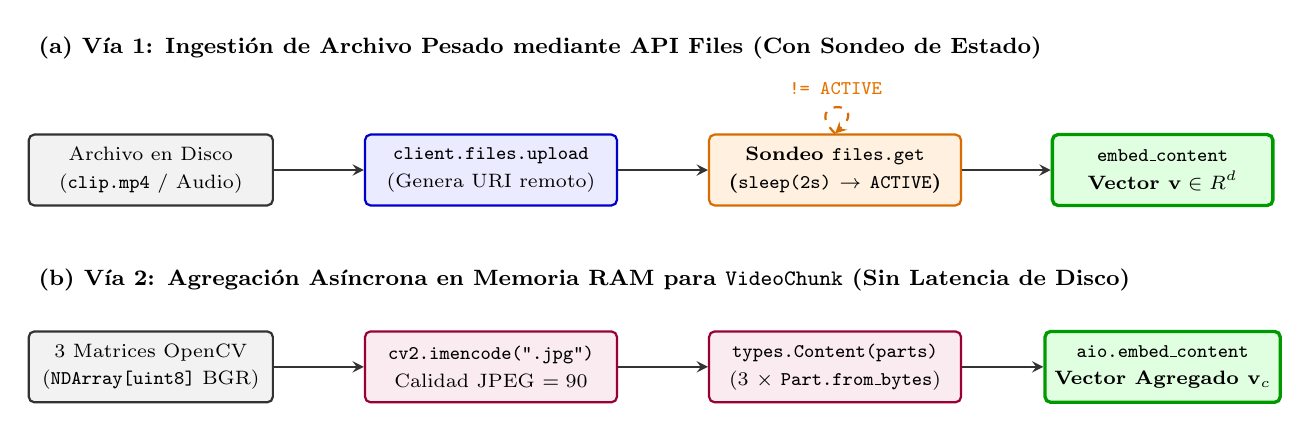
\begin{tikzpicture}[
    node distance=0.5cm and 0.65cm,
    box/.style={rectangle, draw=black!80, fill=gray!10, thick, minimum width=3.1cm, minimum height=0.90cm, align=center, font=\scriptsize, rounded corners=2pt},
    cloudbox/.style={rectangle, draw=blue!80!black, fill=blue!8, thick, minimum width=3.2cm, minimum height=0.90cm, align=center, font=\scriptsize, rounded corners=2pt},
    statebox/.style={rectangle, draw=orange!85!black, fill=orange!12, thick, minimum width=3.2cm, minimum height=0.90cm, align=center, font=\scriptsize\bfseries, rounded corners=2pt},
    membox/.style={rectangle, draw=purple!80!black, fill=purple!8, thick, minimum width=3.2cm, minimum height=0.90cm, align=center, font=\scriptsize, rounded corners=2pt},
    outbox/.style={rectangle, draw=green!60!black, fill=green!12, very thick, minimum width=2.8cm, minimum height=0.90cm, align=center, font=\scriptsize\bfseries, rounded corners=2pt},
    arrow/.style={-stealth, thick, draw=black!80}
]
% Vía A: API Files
\node[font=\bfseries\footnotesize, anchor=west] at (-7.9, 3.35) {(a) Vía 1: Ingestión de Archivo Pesado mediante API Files (Con Sondeo de Estado)};
\node[box] (f_disk) at (-6.35, 1.80) {Archivo en Disco\\[2pt](\texttt{clip.mp4} / Audio)};
\node[cloudbox] (f_up) at (-2.03, 1.80) {\texttt{client.files.upload}\\[2pt](Genera URI remoto)};
\node[statebox] (f_poll) at (2.34, 1.80) {Sondeo \texttt{files.get}\\[2pt](\texttt{sleep(2s)} $\to$ \texttt{ACTIVE})};
\node[outbox] (f_emb) at (6.50, 1.80) {\texttt{embed\_content}\\[2pt]Vector $\mathbf{v} \in \mathbb{R}^d$};

\draw[arrow] (f_disk) -- (f_up);
\draw[arrow] (f_up) -- (f_poll);
\draw[arrow] (f_poll) -- (f_emb);
\draw[arrow, dashed, orange!85!black] (f_poll.north) .. controls (1.9, 2.70) and (2.8, 2.70) .. node[above=1pt, font=\scriptsize\bfseries, text=orange!90!black] {\texttt{!= ACTIVE}} (f_poll.north);

% Vía B: Agregación en Memoria
\node[font=\bfseries\footnotesize, anchor=west] at (-7.9, 0.40) {(b) Vía 2: Agregación Asíncrona en Memoria RAM para \texttt{VideoChunk} (Sin Latencia de Disco)};
\node[box] (m_cv) at (-6.35, -0.70) {3 Matrices OpenCV\\[2pt](\texttt{NDArray[uint8]} BGR)};
\node[membox] (m_jpg) at (-2.03, -0.70) {\texttt{cv2.imencode(".jpg")}\\[2pt]Calidad JPEG $= 90$};
\node[membox] (m_part) at (2.34, -0.70) {\texttt{types.Content(parts)}\\[2pt](3 $\times$ \texttt{Part.from\_bytes})};
\node[outbox] (m_emb) at (6.50, -0.70) {\texttt{aio.embed\_content}\\[2pt]Vector Agregado $\mathbf{v}_c$};

\draw[arrow] (m_cv) -- (m_jpg);
\draw[arrow] (m_jpg) -- (m_part);
\draw[arrow] (m_part) -- (m_emb);
\end{tikzpicture}
\caption{Comparativa técnica de los dos flujos de ingestión en el SDK \texttt{google-genai}: (a) subida de archivos completos a la API Files con bucle de espera activa hasta alcanzar el estado \texttt{ACTIVE}, y (b) codificación JPEG en memoria de múltiples fotogramas empaquetados en un único objeto \texttt{types.Content} para llamadas asíncronas de baja latencia \cite{gemini_emb2_docs}.} %[cite: 3]
\label{fig:gemini_ingest_modes}
\end{figure}

Asimismo, para cerrar el ciclo de búsqueda cruzada y multimodal, el mismo componente vectorizador expone el método \texttt{embed\_query} (respaldado por \texttt{build\_query\_payload} y manteniendo \texttt{embed\_text} por retrocompatibilidad), capaz de empaquetar en un único contenedor \texttt{types.Content} cualquier combinación de consulta textual, ficheros \texttt{.txt}, imágenes de referencia codificadas a JPEG (\texttt{types.Part.from\_bytes}) y transcripciones de pistas de audio de entrada obtenidas con \texttt{transcribe\_query\_audios}. Al invocar \texttt{aio.models.embed\_content} en una sola llamada de red con idéntica configuración dimensional (\texttt{output\_dimensionality}) y normalización $L_2$, el sistema garantiza la compatibilidad algebraica exacta entre los fragmentos de vídeo indexados y las consultas multimodales del usuario \cite{gemini_emb2_docs}. %[cite: 3]

\subsubsection{Modelado Matemático de Cuotas Operativas (RPM, TPM y RPD) y Planificación de Capacidad}
\label{subsubsec:modelado_cuotas_capacidad}

Un aspecto crítico en el diseño de arquitecturas de ingeniería basadas en modelos fundacionales en la nube es la caracterización matemática de los límites de tasa (\textit{Rate Limits}) impuestos por el proveedor del servicio \cite{gemini_emb2_docs}. %[cite: 3]
En el entorno de experimentación y validación de Google AI Studio (capa gratuita o \textit{Free Tier}) para el modelo \texttt{gemini-embedding-2-preview}, la infraestructura impone simultáneamente tres umbrales restrictivos \cite{gemini_emb2_docs}: %[cite: 3]
\begin{itemize}
    \item \textbf{RPM (\textit{Requests Per Minute}):} Límite máximo de $\text{RPM}_{\max} = 100$ peticiones por minuto \cite{gemini_emb2_docs}. %[cite: 3]
    \item \textbf{TPM (\textit{Tokens Per Minute}):} Límite máximo de $\text{TPM}_{\max} = 30.000$ \textit{tokens} procesados por minuto \cite{gemini_emb2_docs}. %[cite: 3]
    \item \textbf{RPD (\textit{Requests Per Day}):} Límite máximo acumulado de $\text{RPD}_{\max} = 1.000$ peticiones por día \cite{gemini_emb2_docs}. %[cite: 3]
\end{itemize}

Un análisis superficial podría sugerir que el sistema es capaz de vectorizar $100$ fragmentos de vídeo (\texttt{VideoChunk}) por minuto atenidos al umbral de $\text{RPM}_{\max} = 100$. %[cite: 3]
Sin embargo, el modelado riguroso de la carga útil multimedia demuestra que el verdadero cuello de botella por minuto reside en el consumo de \textit{tokens} ($\text{TPM}_{\max}$) \cite{gemini_emb2_docs}. %[cite: 3]
Cada imagen o fotograma enviado a los modelos de la familia Gemini consume una tasa base de aproximadamente $T_{\text{img}} \approx 258\text{--}300$ \textit{tokens} \cite{gemini_emb2_docs}. %[cite: 3]
Dado que el algoritmo de selección por entropía extrae $N_{\text{frames}} = 3$ fotogramas clave por cada \texttt{VideoChunk}, el coste en \textit{tokens} de una única petición de fragmento asciende según la Ecuación~\eqref{eq:tokens_por_chunk} a: %[cite: 3]

\begin{equation}
T_{\text{chunk}} = N_{\text{frames}} \times T_{\text{img}} \approx 3 \times 300 = 900 \text{ tokens/chunk}
\label{eq:tokens_por_chunk}
\end{equation} %[cite: 3]

Si el orquestador enviase el máximo permitido de $100$ peticiones en un minuto, la demanda de caudal ascendería a $100 \times 900 = 90.000$ \textit{tokens}/minuto, triplicando el límite de $\text{TPM}_{\max} = 30.000$ y provocando el rechazo inmediato de las peticiones con código de error HTTP \texttt{429 (Too Many Requests)}. %[cite: 3]
En consecuencia, el caudal máximo efectivo sostenido ($\lambda_{\text{efectivo}}$) en fragmentos por minuto queda determinado según la Ecuación~\eqref{eq:caudal_efectivo_chunks} por el mínimo entre la restricción de peticiones y la restricción de \textit{tokens}: %[cite: 3]

\begin{equation}
\lambda_{\text{efectivo}} = \min\!\left(\text{RPM}_{\max}, \, \left\lfloor \frac{\text{TPM}_{\max}}{T_{\text{chunk}}} \right\rfloor\right) = \min\!\left(100, \, \left\lfloor \frac{30.000}{900} \right\rfloor\right) \approx 33 \text{ chunks/minuto}
\label{eq:caudal_efectivo_chunks}
\end{equation} %[cite: 3]

Esto restringe la velocidad de ingestión real a un rango de entre $30$ y $35$ fragmentos de vídeo por minuto, lo que significa que un vídeo de prueba que genere entre $100$ y $200$ \textit{chunks} requerirá entre $3$ y $6$ minutos de procesamiento continuo. %[cite: 3]

De forma análoga, el límite diario de $\text{RPD}_{\max} = 1.000$ peticiones acota la duración máxima de vídeo que puede indexarse en una jornada de experimentación. %[cite: 3]
Bajo una segmentación semántica adaptativa (\textit{Video-RAC}), un vídeo educativo o divulgativo promedio experimenta un cambio de plano cada $\bar{d}_{\text{plano}} \in [3, 7]$ segundos. %[cite: 3]
Asumiendo una media conservadora de $\bar{d}_{\text{plano}} = 5$ segundos por fragmento, cada minuto de metraje produce $C_{\text{min}} = 60 / 5 = 12$ \textit{chunks}/minuto, lo que arroja un límite teórico absoluto de duración diaria ($D_{\max}$) formulado en la Ecuación~\eqref{eq:duracion_maxima_diaria}: %[cite: 3]

\begin{equation}
D_{\max} = \frac{\text{RPD}_{\max}}{C_{\text{min}}} = \frac{1.000 \text{ chunks/día}}{12 \text{ chunks/minuto}} \approx 83,3 \text{ minutos/día}
\label{eq:duracion_maxima_diaria}
\end{equation} %[cite: 3]

Para evitar que el procesamiento accidental de un único archivo de larga duración agote el $100\%$ de la cuota diaria e impida realizar búsquedas o iteraciones de calibración durante el resto del día, la arquitectura de ingeniería implementa dos salvaguardas: acotar los vídeos de validación de la Prueba de Concepto a clips de entre \textbf{5 y 15 minutos} (que generan entre $100$ y $200$ \textit{chunks}, consumiendo apenas un $10\%\text{--}20\%$ del RPD), e incorporar en el orquestador un cortafuegos estático (\textit{fail-safe}) definido por la constante \texttt{MAX\_CHUNKS\_PER\_VIDEO = 800}. %[cite: 3]
Si tras la detección de bordes de plano con OpenCV el vídeo supera los $800$ fragmentos, el sistema aborta preventivamente lanzando la excepción \texttt{QuotaSafetyError} antes de extraer fotogramas ni consumir una sola petición de la API. %[cite: 3]

La Figura~\ref{fig:cuello_botella_tpm_rpd} esquematiza la interacción entre los tres umbrales de cuota y los mecanismos de protección implementados en el flujo de ingestión. %[cite: 3]

\begin{figure}[htbp]
\centering
\begin{tikzpicture}[
    node distance=0.5cm and 0.7cm,
    innode/.style={rectangle, draw=black!80, fill=gray!10, thick, minimum width=3.0cm, minimum height=1.2cm, align=center, font=\scriptsize, rounded corners=2pt},
    guardnode/.style={diamond, aspect=2.0, draw=red!80!black, fill=red!8, very thick, minimum width=2.8cm, minimum height=1.3cm, align=center, font=\scriptsize\bfseries},
    limitbox/.style={rectangle, draw=blue!80!black, fill=blue!8, thick, minimum width=4.0cm, minimum height=1.9cm, align=center, font=\scriptsize, rounded corners=3pt},
    abortbox/.style={rectangle, draw=red!80!black, fill=red!12, very thick, minimum width=3.2cm, minimum height=1.0cm, align=center, font=\scriptsize\bfseries, rounded corners=2pt},
    okbox/.style={rectangle, draw=green!60!black, fill=green!12, very thick, minimum width=4.0cm, minimum height=1.3cm, align=center, font=\scriptsize\bfseries, rounded corners=2pt},
    arrow/.style={-stealth, thick, draw=black!80}
]
\node[innode] (vid) at (-5.1, 0.0) {\textbf{Vídeo Segmentado}\\[2pt]$N$ \texttt{VideoChunks}\\($\sim 12$ chunks/min)};

\node[guardnode] (guard) at (-1.0, 0.0) {¿$N > 800$?\\(\texttt{MAX\_CHUNKS})};

\node[abortbox] (abort) at (-1.0, 2.1) {\texttt{QuotaSafetyError}\\[2pt]Aborta sin gastar API\\(Protege 1.000 RPD)};

\node[limitbox] (tpm) at (4.5, 0.0) {\textbf{Control de Caudal API}\\[2pt]
$\bullet$ $\text{RPM}_{\max} = 100$ pet/min\\[1pt]
$\bullet$ $\text{TPM}_{\max} = 30.000$ tok/min\\[1pt]
$\bullet$ Coste $\approx 900$ tok/chunk\\[2pt]
\textbf{Techo real: $\sim 33$ chunks/min}};

\node[okbox] (out) at (4.5, -2.35) {\textbf{Ingestión Controlada}\\[2pt]Clips 5-15 min (100-200 chunks)\\[1pt]Consumo: 10\%-20\% RPD};

\draw[arrow] (vid) -- (guard);
\draw[arrow, draw=red!80!black] (guard) -- node[right=3pt, font=\scriptsize\bfseries, text=red!80!black] {Sí} (abort);
\draw[arrow, draw=green!50!black] (guard) -- node[above=2pt, font=\scriptsize\bfseries, text=green!50!black] {No ($\le 800$)} (tpm);
\draw[arrow] (tpm) -- (out);
\end{tikzpicture}
\caption{Modelado de capacidad y cortafuegos de cuota para \texttt{gemini-embedding-2-preview}: la validación previa aborta ejecuciones que superen los $800$ fragmentos para proteger el límite diario (1.000 RPD), mientras que la densidad de $\sim 900$ \textit{tokens} por fragmento fija el caudal efectivo en $\sim 33$ \textit{chunks}/minuto bajo el techo de 30.000 TPM \cite{gemini_emb2_docs}.} %[cite: 3]
\label{fig:cuello_botella_tpm_rpd}
\end{figure}

\subsubsection{Ingeniería de Resiliencia: Control de Concurrencia, Ventana de \textit{Backoff} de 60 Segundos y Degradación Elegante}
\label{subsubsec:resiliencia_backoff_degradacion}

Dado que el procesamiento de vídeo combina operaciones intensivas de CPU (decodificación de fotogramas y cálculo de mapas gaussianos SSIM en OpenCV) con operaciones asíncronas de red (llamadas HTTP a la API de Gemini), la arquitectura de software debe evitar tanto el bloqueo del bucle de eventos como la saturación de los servidores remotos. %[cite: 3]

En primer lugar, las funciones síncronas bloqueantes de visión por computador (\texttt{detect\_shot\_boundaries} y \texttt{extract\_key\_frames}) se delegan a hilos secundarios mediante \texttt{asyncio.to\_thread}, liberando el hilo principal de Python para gestionar las conexiones de red. %[cite: 3]
En segundo lugar, la emisión paralela de tareas de vectorización en \texttt{asyncio.gather} se regula mediante un semáforo asíncrono (\texttt{asyncio.Semaphore(max\_concurrent\_requests)}) calibrado específicamente en \texttt{max\_concurrent\_requests = 3} (reducido respecto a un valor inicial de $5$) para impedir ráfagas instantáneas que desborden las cuotas por minuto. %[cite: 3]

Pese al uso del semáforo, dado que la latencia de respuesta de una petición individual es inferior a un segundo, tres corrutinas concurrentes pueden alcanzar el techo de $30.000$ \textit{tokens} antes de que se cumpla el minuto natural, recibiendo un error transitorio HTTP \texttt{429}. %[cite: 3]
Para absorber este fenómeno sin perder datos (así como fallos transitorios de servidor catalogados en el conjunto inmutable \texttt{\_RETRYABLE\_CODES = \{429, 500, 502, 503, 504\}} y errores de red \texttt{OSError}/\texttt{TimeoutError}), el método privado \texttt{\_embed} implementa un algoritmo de \textbf{reintento con espera exponencial (\textit{Exponential Backoff})}. %[cite: 3]

La calibración matemática de los parámetros de este \textit{backoff} resulta determinante: si se utilizase una espera base de $t_0 = 2,0\text{ s}$ con $R = 3$ reintentos, la suma de las pausas sería únicamente de $2 + 4 + 8 + 16 = 28\text{ s}$ (o $2+4+8 = 14\text{ s}$ en tres esperas), tiempo insuficiente para que Google reinicie la ventana deslizante de $60$ segundos del límite TPM. %[cite: 3]
Por el contrario, al incrementar los parámetros por defecto a un retardo base de \texttt{retry\_base\_delay} $= 4,0\text{ s}$ y un máximo de \texttt{max\_retries} $= 4$ reintentos, el tiempo de espera en el intento $k \in \{0, 1, 2, 3\}$ responde a $\Delta t_k = 4,0 \times 2^k$, generando una ventana acumulada calculada según la Ecuación~\eqref{eq:suma_backoff_60s}: %[cite: 3]

\begin{equation}
T_{\text{espera total}} = \sum_{k=0}^{3} t_0 \cdot 2^k = 4,0 \times (2^0 + 2^1 + 2^2 + 2^3) = 4 + 8 + 16 + 32 = 60 \text{ segundos}
\label{eq:suma_backoff_60s}
\end{equation} %[cite: 3]

La Figura~\ref{fig:backoff_ventana_60s} muestra cómo esta progresión geométrica cubre exactamente los $60$ segundos necesarios para garantizar la renovación de la cuota de \textit{tokens} por minuto antes de agotar el último intento. %[cite: 3]

\begin{figure}[htbp]
\centering
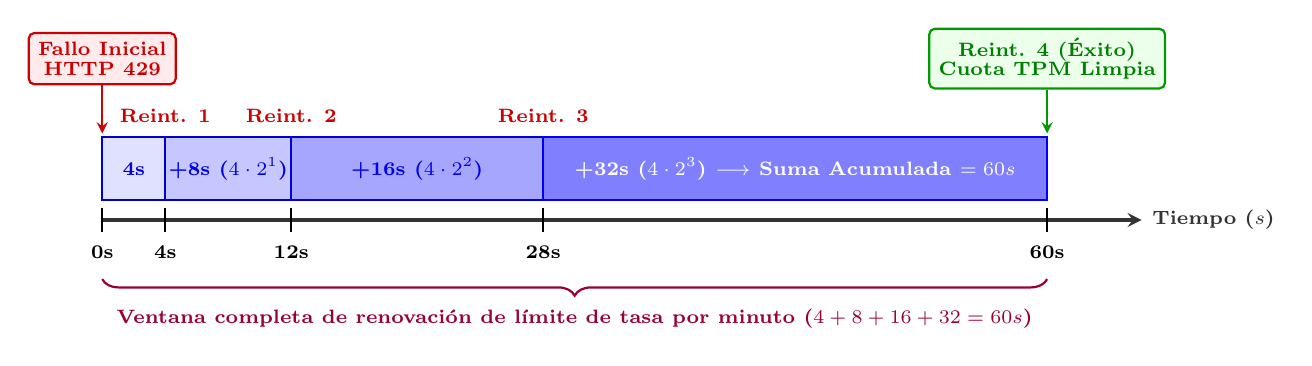
\begin{tikzpicture}
% Línea base de tiempo (0 a 60 segundos)
\draw[-stealth, very thick, black!80] (0,0) -- (13.2,0) node[right, font=\scriptsize\bfseries] {Tiempo ($s$)};

% Marcas de tiempo proporcionales (escala: 1 seg = 0.2 unidades -> 60s = 12.0 unidades)
\foreach \x/\t in {0/0s, 0.8/4s, 2.4/12s, 5.6/28s, 12.0/60s} {
    \draw[thick, black] (\x, 0.15) -- (\x, -0.15);
    \node[below, font=\scriptsize\bfseries] at (\x, -0.2) {\t};
}

% Bloques de espera exponencial
\draw[fill=blue!12, draw=blue!80!black, thick] (0, 0.25) rectangle (0.8, 1.05);
\node[font=\scriptsize\bfseries, blue!90!black] at (0.4, 0.65) {4s};

\draw[fill=blue!22, draw=blue!80!black, thick] (0.8, 0.25) rectangle (2.4, 1.05);
\node[font=\scriptsize\bfseries, blue!90!black] at (1.6, 0.65) {+8s ($4\cdot 2^1$)};

\draw[fill=blue!35, draw=blue!85!black, thick] (2.4, 0.25) rectangle (5.6, 1.05);
\node[font=\scriptsize\bfseries, blue!95!black] at (4.0, 0.65) {+16s ($4\cdot 2^2$)};

\draw[fill=blue!50, draw=blue!95!black, thick] (5.6, 0.25) rectangle (12.0, 1.05);
\node[font=\scriptsize\bfseries, white] at (8.8, 0.65) {+32s ($4\cdot 2^3$) $\longrightarrow$ Suma Acumulada $= 60\text{ s}$};

% Eventos de fallo e intento exitoso
\node[draw=red!80!black, fill=red!8, thick, rounded corners=2pt, font=\scriptsize\bfseries, text=red!80!black, align=center] (fail0) at (0.0, 2.05) {Fallo Inicial\\[-1pt]HTTP 429};
\draw[-stealth, thick, red!80!black] (fail0.south) -- (0.0, 1.10);

\node[above=2pt, font=\scriptsize\bfseries, text=red!80!black] at (0.8, 1.05) {Reint. 1};
\node[above=2pt, font=\scriptsize\bfseries, text=red!80!black] at (2.4, 1.05) {Reint. 2};
\node[above=2pt, font=\scriptsize\bfseries, text=red!80!black] at (5.6, 1.05) {Reint. 3};

\node[draw=green!60!black, fill=green!8, thick, rounded corners=2pt, font=\scriptsize\bfseries, text=green!50!black, align=center] (succ) at (12.0, 2.05) {Reint. 4 (Éxito)\\[-1pt]Cuota TPM Limpia};
\draw[-stealth, thick, green!60!black] (succ.south) -- (12.0, 1.10);

% Llave inferior de ventana de 1 minuto
\draw[decorate, decoration={brace, amplitude=6pt, mirror}, thick, purple!80!black] (0, -0.75) -- (12.0, -0.75) node[midway, below=7pt, font=\scriptsize\bfseries, purple!80!black] {Ventana completa de renovación de límite de tasa por minuto ($4 + 8 + 16 + 32 = 60\text{ s}$)};
\end{tikzpicture}
\caption{Cronograma temporal del algoritmo de \textit{Exponential Backoff} calibrado (\texttt{retry\_base\_delay = 4.0}, \texttt{max\_retries = 4}): la suma geométrica de las cuatro esperas alcanza exactamente $60$ segundos, permitiendo superar bloqueos completos de la ventana de 30.000 TPM sin abortar la vectorización del fragmento.} %[cite: 3]
\label{fig:backoff_ventana_60s}
\end{figure}

Adicionalmente, el diseño incorpora dos mecanismos de \textbf{Degradación Elegante (\textit{Graceful Degradation})} en distintas capas del sistema para garantizar una tolerancia a fallos de nivel industrial: %[cite: 3]
\begin{enumerate}
    \item \textbf{Aislamiento de fallos parciales en la fase de ingestión (\texttt{return\_exceptions=True}):} Si tras agotar los $60$ segundos de reintentos un fragmento puntual sigue fallando (lanzando \texttt{VectorizationError}), la invocación \texttt{asyncio.gather(* tasks, return\_exceptions=True)} evita que se cancele el lote completo. %[cite: 3]
    El orquestador captura la excepción de ese único \textit{chunk}, la documenta en \texttt{execution.log} mediante el auditor (\texttt{RunAuditor}) y conserva intactos todos los demás fragmentos vectorizados del vídeo. %[cite: 3]
    \item \textbf{Respaldo vectorial ante caídas \texttt{503 UNAVAILABLE} en la segunda etapa de reordenación visual:} Durante la fase de búsqueda y refinamiento con modelos ligeros de visión-lenguaje (como \texttt{gemini-3.5-flash-lite}), los servidores de Google pueden experimentar picos temporales de demanda devolviendo el error \texttt{503 UNAVAILABLE ("This model is currently experiencing high demand")}. %[cite: 3]
    Cuando esto ocurre y se agotan los reintentos del verificador secundario, el sistema no colapsa ni devuelve un error al usuario: intercepta la indisponibilidad, emite un aviso informando que la reordenación visual no está disponible temporalmente y \textbf{conserva automáticamente el orden vectorial original devuelto por Qdrant} en la primera etapa. %[cite: 3]
\end{enumerate}

La Figura~\ref{fig:degradacion_elegante_503} representa este flujo de continuidad operativa y degradación elegante en ambas fases de la arquitectura. %[cite: 3]

\begin{figure}[htbp]
\centering
\begin{tikzpicture}[
    node distance=0.5cm and 0.65cm,
    proc/.style={rectangle, draw=blue!80!black, fill=blue!8, thick, minimum width=3.1cm, minimum height=1.1cm, align=center, font=\scriptsize, rounded corners=2pt},
    dec/.style={diamond, aspect=1.9, draw=orange!85!black, fill=orange!10, thick, minimum width=2.3cm, minimum height=1.2cm, align=center, font=\scriptsize\bfseries},
    warn/.style={rectangle, draw=purple!80!black, fill=purple!10, thick, minimum width=3.2cm, minimum height=1.2cm, align=center, font=\scriptsize, rounded corners=2pt},
    ok/.style={rectangle, draw=green!60!black, fill=green!12, very thick, minimum width=3.2cm, minimum height=1.2cm, align=center, font=\scriptsize, rounded corners=2pt},
    arrow/.style={-stealth, thick, draw=black!80}
]
\node[proc] (qdrant) at (-6.25, 0.0) {\textbf{1.ª Etapa: Qdrant}\\[2pt]Recupera Top-$K$ por\\Similitud Coseno};

\node[proc] (rerank) at (-1.95, 0.0) {\textbf{2.ª Etapa: Verificador}\\[2pt]{\scriptsize \texttt{gemini-3.5-flash-lite}}\\[1pt]+ Backoff Exponencial};

\node[dec] (status) at (1.90, 0.0) {¿HTTP 503\\Persiste?};

\node[warn] (fallback) at (1.90, 2.1) {\textbf{Degradación Elegante}\\[2pt]Log: \textit{Fallo 503 VLM}\\[1pt]Omite filtro secundario};

\node[ok] (out_rerank) at (6.20, 0.0) {\textbf{Resultados Top-}$K$\\[2pt]Reordenados por VLM\\(Máxima precisión)};

\node[ok, draw=teal!80!black, fill=teal!12] (out_vec) at (6.20, 2.1) {\textbf{Resultados Top-}$K$\\[2pt]Orden Vectorial Original\\(Preserva ranking Qdrant)};

\draw[arrow] (qdrant) -- (rerank);
\draw[arrow] (rerank) -- (status);
\draw[arrow, draw=red!80!black] (status) -- node[right=3pt, font=\scriptsize\bfseries, text=red!80!black] {Sí (503)} (fallback);
\draw[arrow, draw=green!50!black] (status) -- node[above=2pt, font=\scriptsize\bfseries, text=green!50!black] {No (200 OK)} (out_rerank);
\draw[arrow, draw=purple!80!black] (fallback) -- (out_vec);
\end{tikzpicture}
\caption{Arquitectura de Degradación Elegante (\textit{Graceful Degradation}) durante la búsqueda: si los servidores del modelo secundario (\texttt{gemini-3.5-flash-lite}) sufren picos de saturación (\texttt{503 UNAVAILABLE}) tras agotar los reintentos, el sistema conmuta limpiamente al orden de similitud vectorial calculado por Qdrant con \textit{Gemini Embedding 2}.} %[cite: 3]
\label{fig:degradacion_elegante_503}
\end{figure}

El Cuadro~\ref{tab:parametros_gemini_vectorizer} sintetiza los parámetros definitivos de ingeniería calibrados en el sistema para maximizar la fiabilidad bajo las restricciones operativas de la API de Google. %[cite: 3]

\begin{table}[htbp]
\centering
\small
\caption{Parámetros técnicos calibrados en los módulos de vectorización y orquestación para operar con \texttt{gemini-embedding-2-preview} sin colapsos de cuota \cite{gemini_emb2_docs}.} %[cite: 3]
\label{tab:parametros_gemini_vectorizer}
\begin{tabularx}{\linewidth}{p{4.2cm}p{3.2cm}p{2.6cm}X}
\toprule
\textbf{Parámetro} & \textbf{Módulo} & \textbf{Valor} & \textbf{Justificación Técnica / MLOps} \\
\midrule
\texttt{model} & \texttt{gemini\_vectorizer.py} & \texttt{gemini-embedding-2} & Modelo omnimodal nativo (espacio compartido) \\
\texttt{output\_dimensionality} & \texttt{gemini\_vectorizer.py} & $3.072$, $1.536$ o $768$ & MRL con normalización $L_2$ (\texttt{truncate\_and\_normalize\_mrl}) \\
\texttt{jpeg\_quality} & \texttt{gemini\_vectorizer.py} & $90$ (escala $1\text{-}100$) & Alta fidelidad visual en RAM sin artefactos \\
\texttt{max\_concurrent\_requests} & \texttt{pipeline.py} & $3$ (reducido de $5$) & Limita peticiones concurrentes en semáforo \\
\texttt{retry\_base\_delay} & \texttt{gemini\_vectorizer.py} & $4,0\text{ s}$ (antes $2,0\text{ s}$) & Base geométrica para cubrir ventana TPM \\
\texttt{max\_retries} & \texttt{gemini\_vectorizer.py} & $4$ (antes $3$) & Suma $4+8+16+32 = 60\text{ s}$ ante error HTTP \\
\texttt{MAX\_CHUNKS\_PER\_VIDEO} & \texttt{pipeline.py} & $800$ fragmentos & Cortafuegos \texttt{QuotaSafetyError} (protege RPD) \\
\bottomrule
\end{tabularx}
\end{table}

% Bloque 2.4: Ecosistema de Modelos Alternativos: Open-Weights y Edge Computing (Págs. 16-20)
% =============================================================================
% CAPÍTULO 2 - BLOQUE 2.4: ECOSISTEMA DE MODELOS ALTERNATIVOS:
% PESOS ABIERTOS (QWEN3-VL), ADAPTACIÓN DE VLMS Y ENTORNOS DE RECURSOS LIMITADOS
% =============================================================================

\subsection{Ecosistema de Modelos Alternativos: Pesos Abiertos (\textit{Open-Weights}) y Ejecución Local}
\label{subsec:modelos_locales}

\subsubsection{Las Dos Macrotendencias de 2026: APIs Propietarias Hiper-escaladas frente a Pesos Abiertos}
\label{subsubsec:macrotendencias_2026}

En el diseño de una plataforma de recuperación profunda de vídeo, la elección de la arquitectura del modelo de \textit{embedding} subyacente constituye el factor crítico que define los límites de escalabilidad, la precisión en la localización de eventos y el coste computacional del sistema \cite{gemini_emb2_docs}. %[cite: 4, 5]
El estado del arte tecnológico en 2026 se estructura en torno a dos macrotendencias complementarias \cite{qwen3_vl_emb2026, gemini_emb2_docs}: %
\begin{enumerate}
    \item \textbf{Modelos Propietarios Hiper-escalados vía API (\textit{Cloud}):} Representados por servicios como \textit{Google Gemini Embedding 2} (\texttt{gemini-embedding-2-preview}), donde la complejidad de la infraestructura de aceleradores (TPUs/GPUs) queda abstraída tras llamadas HTTP, ofreciendo espacios vectoriales masivos de hasta $3.072$ dimensiones con soporte nativo para vídeo, audio, imagen, texto y documentos PDF \cite{gemini_emb2_docs, openrouter_gemini_emb2}. %[cite: 3, 4]
    \item \textbf{Ecosistemas de Pesos Abiertos (\textit{Open-Weights}) y Despliegue Local:} Integrados por familias de modelos cuyos pesos neuronales son públicamente accesibles en repositorios como Hugging Face (destacando la serie \textbf{Qwen3-VL-Embedding} y \textbf{Qwen3-VL-Reranker}, arquitecturas como \textbf{ColQwen} y variantes ligeras de la familia \textbf{Gemma}), los cuales pueden ejecutarse en servidores locales propios o en instancias privadas sin depender de proveedores externos \cite{qwen3_vl_emb2026, hf_train_multimodal2026, prajwal2025multimodal}. %[cite: 3, 4]
\end{enumerate}

Un hallazgo fundamental documentado en la literatura del primer trimestre de 2026 es que las implementaciones de código abierto han logrado cerrar la brecha histórica de rendimiento frente a las APIs propietarias en tareas de recuperación multimodal \cite{qwen3_vl_emb2026, alphaxiv_qwen3}. %[cite: 4]
Esta convergencia técnica tiene una repercusión directa en el ámbito universitario e industrial: posibilita el diseño de infraestructuras de investigación académica y de producción que no dependen del pago continuo por inferencia (\textit{pay-per-token}) ni se ven estranguladas por límites diarios de peticiones, garantizando además la soberanía y privacidad absoluta sobre archivos de vídeo sensibles \cite{qwen3_vl_emb2026}. %[cite: 3, 4]

La Figura~\ref{fig:ecosistema_cloud_vs_open} presenta la taxonomía comparada de ambas corrientes tecnológicas dentro del panorama de modelos fundacionales multimodales de 2026. %[cite: 3, 4]

\begin{figure}[htbp]
\centering
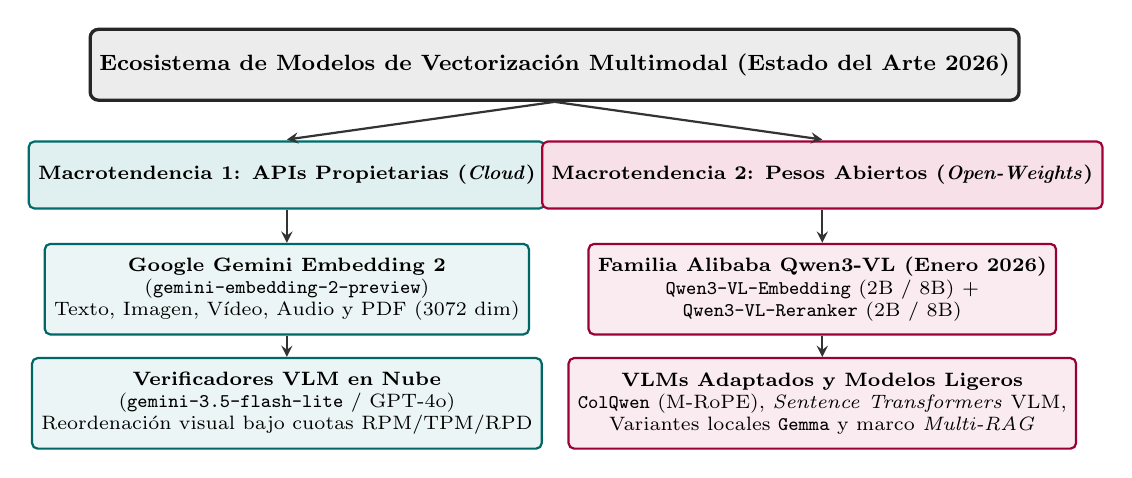
\begin{tikzpicture}[
    node distance=0.5cm and 0.6cm,
    rootbox/.style={rectangle, draw=black!85, fill=gray!15, very thick, minimum width=7.8cm, minimum height=0.9cm, align=center, font=\footnotesize\bfseries, rounded corners=3pt},
    branchbox/.style={rectangle, draw=blue!80!black, fill=blue!10, thick, minimum width=6.0cm, minimum height=0.85cm, align=center, font=\scriptsize\bfseries, rounded corners=2pt},
    leafcloud/.style={rectangle, draw=teal!80!black, fill=teal!8, thick, minimum width=5.8cm, minimum height=1.15cm, align=center, font=\scriptsize, rounded corners=2pt},
    leafopen/.style={rectangle, draw=purple!80!black, fill=purple!8, thick, minimum width=5.8cm, minimum height=1.15cm, align=center, font=\scriptsize, rounded corners=2pt},
    arrow/.style={-stealth, thick, draw=black!80}
]
\node[rootbox] (root) at (0, 3.2) {Ecosistema de Modelos de Vectorización Multimodal (Estado del Arte 2026)};

% Ramas principales
\node[branchbox, draw=teal!85!black, fill=teal!12] (cloud) at (-3.4, 1.8) {Macrotendencia 1: APIs Propietarias (\textit{Cloud})};
\node[branchbox, draw=purple!85!black, fill=purple!12] (open) at (3.4, 1.8) {Macrotendencia 2: Pesos Abiertos (\textit{Open-Weights})};

\draw[arrow] (root.south) -- (-3.4, 2.25);
\draw[arrow] (root.south) -- (3.4, 2.25);

% Hojas Cloud
\node[leafcloud] (c1) at (-3.4, 0.35) {\textbf{Google Gemini Embedding 2}\\(\texttt{gemini-embedding-2-preview})\\Texto, Imagen, Vídeo, Audio y PDF (3072 dim)};
\node[leafcloud] (c2) at (-3.4, -1.1) {\textbf{Verificadores VLM en Nube}\\(\texttt{gemini-3.5-flash-lite} / GPT-4o)\\Reordenación visual bajo cuotas RPM/TPM/RPD};

\draw[arrow] (cloud) -- (c1);
\draw[arrow] (c1) -- (c2);

% Hojas Open-Weights
\node[leafopen] (o1) at (3.4, 0.35) {\textbf{Familia Alibaba Qwen3-VL (Enero 2026)}\\ \texttt{Qwen3-VL-Embedding} (2B / 8B) +\\ \texttt{Qwen3-VL-Reranker} (2B / 8B)};
\node[leafopen] (o2) at (3.4, -1.1) {\textbf{VLMs Adaptados y Modelos Ligeros}\\ \texttt{ColQwen} (M-RoPE), \textit{Sentence Transformers} VLM,\\Variantes locales \texttt{Gemma} y marco \textit{Multi-RAG}};

\draw[arrow] (open) -- (o1);
\draw[arrow] (o1) -- (o2);
\end{tikzpicture}
\caption{Clasificación de las arquitecturas de modelos fundacionales para Video RAG en 2026: coexistencia de modelos hiper-escalados servidos mediante API comercial frente a ecosistemas de pesos abiertos desplegables en infraestructura local \cite{gemini_emb2_docs, qwen3_vl_emb2026, multi_rag2025}.} %[cite: 3, 4]
\label{fig:ecosistema_cloud_vs_open}
\end{figure}

\subsubsection{La Familia Qwen3-VL: Recuperación y Reordenación Multimodal a Escala Masiva}
\label{subsubsec:familia_qwen3_vl}

En el espectro del software libre y los modelos de pesos abiertos, la referencia técnica para la recuperación de información multimodal viene marcada por el lanzamiento en enero de 2026 de la serie \textbf{Qwen3-VL-Embedding} y \textbf{Qwen3-VL-Reranker} por parte del grupo de investigación de Alibaba \cite{qwen3_vl_emb2026, qwen3_vl_blog2026, qwen3_vl_github2026}. %[cite: 4]
Publicados oficialmente en configuraciones de $2.000$ millones (\texttt{Qwen/Qwen3-VL-Embedding-2B}) y $8.000$ millones de parámetros (\texttt{Qwen/Qwen3-VL-Embedding-8B}), junto con adaptaciones especializadas en recuperación de documentos visuales (\texttt{tomaarsen/Qwen3-VL-Embedding-2B-vdr}), estos modelos abordan el problema del RAG sobre grandes repositorios de vídeo mediante un diseño acoplado en dos etapas que supera las limitaciones de latencia de los sistemas generativos directos \cite{qwen3_vl_emb2026, hf_qwen3_2b, hf_qwen3_8b, hf_qwen3_vdr}. %[cite: 4]

\paragraph{Primera Etapa (\texttt{Qwen3-VL-Embedding}):}
Actúa como un codificador denso de doble torre (\textit{Bi-Encoder}) construido sobre la arquitectura base de visión y lenguaje de la familia Qwen3 \cite{qwen3_vl_emb2026, learnopencv_qwen3}. %[cite: 4]
Gracias a la integración nativa de \textit{Multimodal Rotary Position Embeddings} (M-RoPE), el modelo proyecta parches y teselas visuales de imágenes y secuencias de vídeo directamente hacia el mismo espacio semántico continuo del lenguaje sin requerir preprocesamiento OCR intermedio \cite{prajwal2025multimodal, qwen3_vl_emb2026}. %[cite: 4]
Estos vectores se almacenan en bases de datos vectoriales como Qdrant o Milvus, permitiendo realizar búsquedas semánticas directas sobre vídeo bruto a gran velocidad \cite{qwen3_vl_emb2026}. %[cite: 3, 4]

\paragraph{Segunda Etapa (\texttt{Qwen3-VL-Reranker}) y Resolución de Consultas Composicionales:}
El aporte arquitectónico más relevante de la investigación del equipo Qwen radica en demostrar empíricamente por qué un \textit{Bi-Encoder} aislado resulta insuficiente ante consultas visualmente complejas \cite{learnopencv_qwen3, qwen3_vl_emb2026}. %[cite: 4]
Los codificadores de doble torre tienden a degradar su precisión ante \textbf{consultas altamente composicionales}, perdiendo relaciones espaciales, direccionales o de atributos cruzados; un caso paradigmático documentado en la literatura es la búsqueda de un evento descrito como \textit{``una persona vistiendo una chaqueta roja que se aleja de una furgoneta blanca''} \cite{learnopencv_qwen3}. %[cite: 4]
En un \textit{Bi-Encoder}, un fragmento de vídeo donde aparezca una furgoneta roja y una persona con chaqueta blanca acercándose a ella puede arrojar una similitud del coseno artificialmente alta debido a la presencia conjunta de los mismos sustantivos y colores en el vector global. %[cite: 4]

Para erradicar estos falsos positivos composicionales, \texttt{Qwen3-VL-Reranker} actúa como un filtro de alta precisión sobre el subconjunto top-$K$ recuperado en la primera fase \cite{learnopencv_qwen3, qwen3_vl_emb2026}. %[cite: 4]
Operando bajo una arquitectura de Torre Única (\textit{Cross-Encoder}), el modelo ingiere simultáneamente la consulta textual $Q$ y el fragmento multimedia candidato $D_k$, permitiendo que sus capas de atención cruzada (\textit{Cross-Attention}) interactúen de manera bidireccional y profunda entre cada \textit{token} léxico del texto y cada parche espacial de los fotogramas del vídeo \cite{learnopencv_qwen3, qwen3_vl_emb2026}. %[cite: 4]
En lugar de emitir un vector de representación, la red finaliza prediciendo según la Ecuación~\eqref{eq:qwen3_reranker_logit} un \textbf{\textit{logit} de probabilidad absoluta} que cuantifica la relevancia exacta de la coincidencia entre el evento visual y la estructura sintáctica de la consulta, maximizando la precisión en las primeras posiciones del ranking \cite{learnopencv_qwen3, qwen3_vl_emb2026}. %[cite: 4]

\begin{equation}
P(\text{Relevante} \mid Q, D_k) = \sigma\!\left(z_{\text{logit}}(Q, D_k)\right) = \frac{1}{1 + \exp\!\left(-\mathbf{w}^\top \mathbf{h}_{\text{Cross-Attention}}(Q, D_k)\right)}
\label{eq:qwen3_reranker_logit}
\end{equation} %[cite: 4]

La Figura~\ref{fig:qwen3_vl_composicional} ilustra el mecanismo mediante el cual \texttt{Qwen3-VL-Reranker} desambigua relaciones espaciales y de atributos sobre los candidatos recuperados por \texttt{Qwen3-VL-Embedding}. %[cite: 4]

\begin{figure}[htbp]
\centering
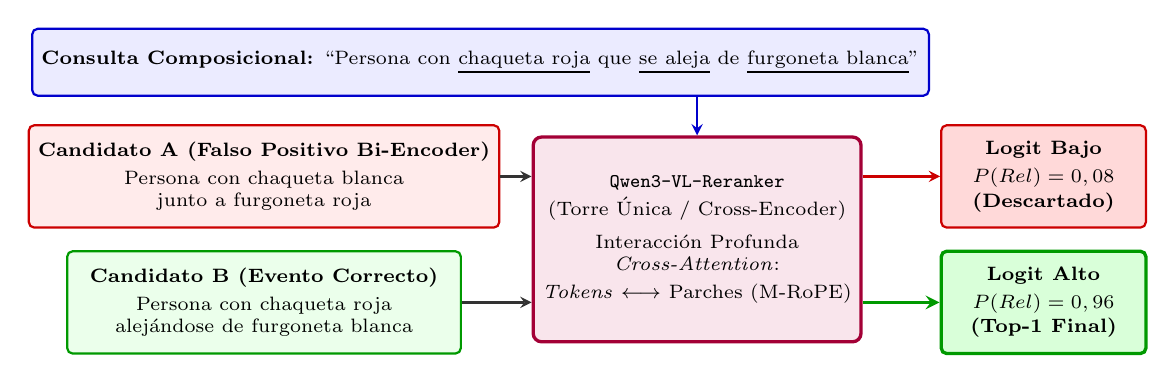
\begin{tikzpicture}[
    node distance=0.5cm and 0.65cm,
    qbox/.style={rectangle, draw=blue!80!black, fill=blue!8, thick, minimum width=10.6cm, minimum height=0.85cm, align=center, font=\scriptsize, rounded corners=2pt},
    candbad/.style={rectangle, draw=red!80!black, fill=red!8, thick, minimum width=5.0cm, minimum height=1.3cm, align=center, font=\scriptsize, rounded corners=2pt},
    candgood/.style={rectangle, draw=green!60!black, fill=green!8, thick, minimum width=5.0cm, minimum height=1.3cm, align=center, font=\scriptsize, rounded corners=2pt},
    attbox/.style={rectangle, draw=purple!85!black, fill=purple!10, very thick, minimum width=3.8cm, minimum height=2.6cm, align=center, font=\scriptsize, rounded corners=3pt},
    outbad/.style={rectangle, draw=red!80!black, fill=red!15, thick, minimum width=2.6cm, minimum height=1.3cm, align=center, font=\scriptsize\bfseries, rounded corners=2pt},
    outgood/.style={rectangle, draw=green!60!black, fill=green!15, very thick, minimum width=2.6cm, minimum height=1.3cm, align=center, font=\scriptsize\bfseries, rounded corners=2pt},
    arrow/.style={-stealth, thick, draw=black!80}
]
% Consulta composicional
\node[qbox] (query) at (-2.25, 2.15) {\textbf{Consulta Composicional:} ``Persona con \underline{chaqueta roja} que \underline{se aleja} de \underline{furgoneta blanca}''};

% Candidatos del Bi-Encoder (Top-K)
\node[candbad] (c1) at (-5.0, 0.70) {\textbf{Candidato A (Falso Positivo Bi-Encoder)}\\[2pt]Persona con chaqueta blanca\\junto a furgoneta roja};
\node[candgood] (c2) at (-5.0, -0.90) {\textbf{Candidato B (Evento Correcto)}\\[2pt]Persona con chaqueta roja\\alejándose de furgoneta blanca};

% Torre Única Qwen3-VL-Reranker
\node[attbox] (rerank) at (0.5, -0.10) {\textbf{\texttt{Qwen3-VL-Reranker}}\\[2pt]
(Torre Única / Cross-Encoder)\\[4pt]
Interacción Profunda\\
\textit{Cross-Attention}:\\[2pt]
\textit{Tokens} $\longleftrightarrow$ Parches (M-RoPE)};

% Salidas de Logit
\node[outbad] (s1) at (4.9, 0.70) {\textbf{Logit Bajo}\\[2pt]$P(\text{Rel}) = 0,08$\\[1pt](Descartado)};
\node[outgood] (s2) at (4.9, -0.90) {\textbf{Logit Alto}\\[2pt]$P(\text{Rel}) = 0,96$\\[1pt](\textbf{Top-1 Final})};

\draw[arrow, blue!80!black, thick] (query.south -| rerank.north) -- (rerank.north);
\draw[arrow] (c1.east) -- (rerank.west |- c1.east);
\draw[arrow] (c2.east) -- (rerank.west |- c2.east);
\draw[arrow, red!80!black, thick] (rerank.east |- s1.west) -- (s1.west);
\draw[arrow, green!60!black, very thick] (rerank.east |- s2.west) -- (s2.west);
\end{tikzpicture}
\caption{Resolución de consultas altamente composicionales mediante la arquitectura en dos etapas de la familia Qwen3-VL: mientras el \textit{Bi-Encoder} puede recuperar candidatos con atributos invertidos, las capas de \textit{Cross-Attention} de \texttt{Qwen3-VL-Reranker} vinculan cada adjetivo y acción con su parche visual exacto para predecir el \textit{logit} de probabilidad real \cite{learnopencv_qwen3, qwen3_vl_emb2026}.} %[cite: 4]
\label{fig:qwen3_vl_composicional}
\end{figure}

\subsubsection{Adaptación de Modelos Visuales (ColQwen y Sentence Transformers) y Entornos Restringidos (\textit{Multi-RAG})}
\label{subsubsec:adaptacion_vlms_multirag}

Más allá de la serie Qwen3-VL, la comunidad investigadora ha consolidado metodologías reproducibles para entrenar y ajustar (\textit{finetuning}) modelos de \textit{embeddings} y \textit{rerankers} multimodales a partir de arquitecturas de lenguaje visual preexistentes, tal y como documenta el marco de \textit{Sentence Transformers} multimodales de Hugging Face \cite{hf_train_multimodal2026, hf_qwen3_paper}. %[cite: 4]

Dentro de esta línea destaca \textbf{ColQwen}, una arquitectura que integra directamente \textit{Multimodal Rotary Position Embeddings} (M-RoPE) sobre el codificador visual para proyectar parches y teselas de documentos complejos, gráficos, ecografías o diapositivas con ecuaciones matemáticas hacia el espacio latente del lenguaje sin pasar por motores OCR \cite{prajwal2025multimodal}. %[cite: 4]
El impacto estructural de este diseño en entornos empresariales y académicos radica en la eliminación de las antiguas cadenas de dependencias compuestas por múltiples APIs de bajo nivel: el modelo fundacional interactúa directamente con la señal visual sin pulir y mapea inherentemente el significado cruzado sin intervención ortográfica, suprimiendo la cascada de errores que un OCR defectuoso propagaba hacia las etapas posteriores del razonamiento algorítmico \cite{prajwal2025multimodal}. %[cite: 4]

La Figura~\ref{fig:finetuning_vlm_to_embedding} esquematiza este flujo de adaptación de un VLM hacia un motor de indexación directa de parches visuales. %[cite: 4]

\begin{figure}[htbp]
\centering

\begin{tikzpicture}[
    rawbox/.style={rectangle, draw=black!80, fill=gray!10, thick, text width=3.1cm, minimum height=1.25cm, align=center, font=\scriptsize, rounded corners=2pt},
    patchbox/.style={rectangle, draw=blue!80!black, fill=blue!8, thick, text width=3.1cm, minimum height=1.25cm, align=center, font=\scriptsize, rounded corners=2pt},
    trainbox/.style={rectangle, draw=orange!85!black, fill=orange!10, thick, text width=3.1cm, minimum height=1.25cm, align=center, font=\scriptsize, rounded corners=2pt},
    spacebox/.style={rectangle, draw=green!60!black, fill=green!12, very thick, text width=3.1cm, minimum height=1.25cm, align=center, font=\scriptsize\bfseries, rounded corners=2pt},
    arrow/.style={-stealth, thick, draw=black!80}
]
\node[rawbox] (in) at (-5.7, 0) {Datos Visuales sin Pulir\\[2pt]{\scriptsize Fotogramas, Gráficos,\\Ecuaciones, Diapositivas}};

\node[patchbox] (vit) at (-1.9, 0) {Partición en Teselas\\[2pt]{\scriptsize \textit{Visual Patches}} +\\[1pt]Rotación \textbf{M-RoPE}};

\node[trainbox] (ft) at (1.9, 0) {Backbone VLM Ajustado\\[2pt]{\scriptsize \textit{ColQwen} / \textit{Qwen3} / \textit{Gemma}}\\[1pt]Sin Etapa OCR};

\node[spacebox] (out) at (5.7, 0) {Proyección Directa al\\Espacio Semántico\\del Lenguaje ($\mathbb{R}^d$)};

\draw[arrow] (in) -- (vit);
\draw[arrow] (vit) -- (ft);
\draw[arrow] (ft) -- (out);
\end{tikzpicture}
\caption{Flujo de codificación visual directa en arquitecturas como \textit{ColQwen} y \textit{Sentence Transformers} multimodales: la combinación de teselas visuales con codificación posicional M-RoPE proyecta diapositivas, gráficos y escenas de vídeo directamente al espacio del lenguaje, eliminando el preprocesamiento intermedio mediante OCR \cite{prajwal2025multimodal, hf_train_multimodal2026}.} %[cite: 4]
\label{fig:finetuning_vlm_to_embedding}
\end{figure}

De manera complementaria, cuando los sistemas deben ejecutarse en dispositivos locales con recursos limitados (escenario donde se ubican las variantes ligeras de ejecución local como la familia \textbf{Gemma} y marcos de trabajo en tiempo real), la literatura reciente aporta la arquitectura \textbf{Multi-RAG} (\textit{A Multimodal Retrieval-Augmented Generation System for Adaptive Video Understanding}) \cite{multi_rag2025, arxiv_adaptive_2505}. %[cite: 3, 4]
\textit{Multi-RAG} introduce una capa de aplicación práctica orientada a la comprensión adaptativa de flujos de vídeo capturados en tiempo real, concebida específicamente como soporte cognitivo para la interacción humano-robot en contextos dinámicos y no estructurados del mundo real \cite{multi_rag2025, arxiv_adaptive_2505}. %[cite: 4]
La aportación fundamental de \textit{Multi-RAG} demuestra que los \textit{embeddings} multimodales son capaces de mantener una inferencia semántica de alto rendimiento incluso cuando la entrada visual se ve temporalmente degradada, ocluida o limitada, validando la robustez de estas representaciones vectoriales en escenarios con fuertes restricciones de recursos computacionales \cite{multi_rag2025, arxiv_adaptive_2505}. %[cite: 4]

\subsubsection{Evaluación en Bancos de Pruebas Masivos (MMEB-V2 y MVEB) y Compromisos de Despliegue}
\label{subsubsec:benchmarks_mmeb_mveb}

Para cuantificar de manera objetiva y estandarizada la capacidad de recuperación de estos modelos fundacionales sobre vídeo, audio y documentos complejos, la comunidad científica ha establecido entre 2025 y 2026 dos bancos de pruebas (\textit{benchmarks}) masivos de referencia \cite{qwen3_vl_emb2026, alphaxiv_qwen3}: %[cite: 3, 4]
\begin{itemize}
    \item \textbf{MMEB-V2 (\textit{Massive Multimodal Embedding Benchmark V2}, 2025):} Amplió la evaluación tradicional de representaciones estáticas texto-imagen para incorporar tareas exigentes de recuperación de fragmentos de vídeo y documentos estructurados (archivos PDF) \cite{qwen3_vl_emb2026, alphaxiv_qwen3}. %[cite: 3, 4]
    Desde el punto de vista metodológico, las métricas empleadas en \textit{MMEB-V2} para clasificación de imágenes y recuperación de vídeo se fundamentan predominantemente en \textbf{\textit{Recall@1}} y \textbf{\textit{Hit@1}}, mientras que los dominios de recuperación de documentos visuales evalúan el ordenamiento mediante \textbf{\textit{NDCG@5}} \cite{alphaxiv_qwen3, qwen3_vl_emb2026}. %[cite: 4]
    \item \textbf{MVEB (\textit{Massive Video Embedding Benchmark}, 2026):} Constituye el estándar específico de evaluación temporal más exhaustivo hasta la fecha, consolidando más de $180$ tareas diferenciadas diseñadas para poner a prueba cómo los modelos de \textit{embeddings} recuperan eventos combinando secuencias de vídeo y pistas de audio. %[cite: 3]
\end{itemize}

A partir de la evidencia empírica recogida en estos bancos de pruebas y de las especificaciones operativas de cada ecosistema, un ingeniero de datos debe ponderar los compromisos arquitectónicos (\textit{trade-offs}) entre desplegar la solución apoyándose en una API propietaria en la nube frente a alojar modelos de pesos abiertos en infraestructura local \cite{gemini_emb2_docs, qwen3_vl_emb2026}. %[cite: 3, 4]
La Figura~\ref{fig:tradeoff_cloud_local_tfm} sintetiza la matriz de decisión técnica entre ambos enfoques. %[cite: 3, 4]

\begin{figure}[htbp]
\centering
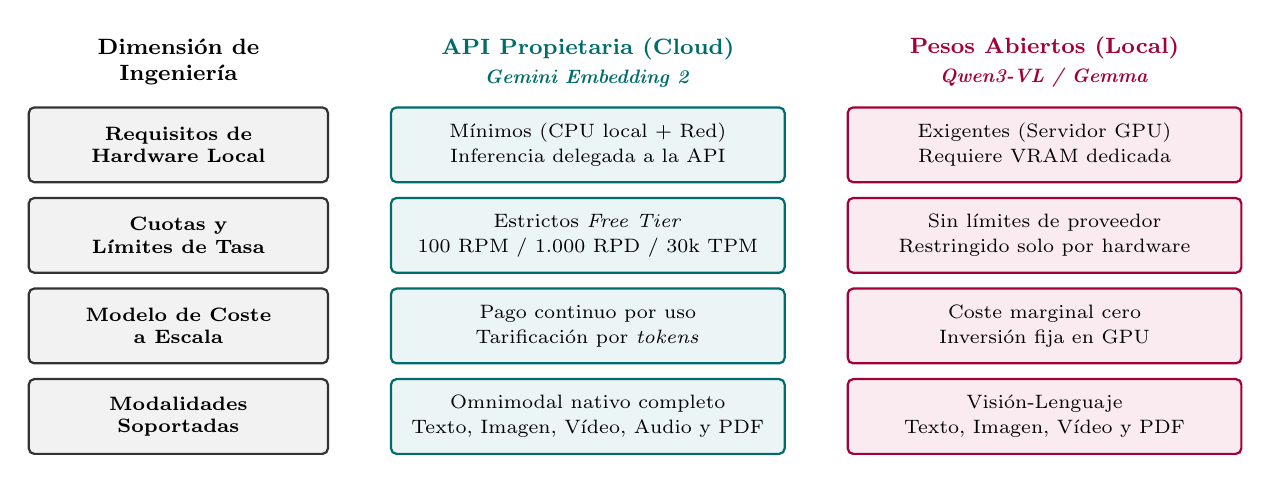
\begin{tikzpicture}[
    node distance=0.5cm and 0.8cm,
    axisbox/.style={rectangle, draw=black!80, fill=gray!10, thick, minimum width=3.8cm, minimum height=0.95cm, align=center, font=\scriptsize\bfseries, rounded corners=2pt},
    cloudnode/.style={rectangle, draw=teal!85!black, fill=teal!8, thick, minimum width=5.0cm, minimum height=0.95cm, align=center, font=\scriptsize, rounded corners=2pt},
    localnode/.style={rectangle, draw=purple!85!black, fill=purple!8, thick, minimum width=5.0cm, minimum height=0.95cm, align=center, font=\scriptsize, rounded corners=2pt}
]
% Encabezados
\node[font=\footnotesize\bfseries, align=center] at (-5.8, 2.35) {Dimensión de\\Ingeniería};
\node[font=\footnotesize\bfseries, teal!85!black, align=center] at (-0.6, 2.35) {API Propietaria (Cloud)\\[1pt]{\scriptsize \textit{Gemini Embedding 2}}};
\node[font=\footnotesize\bfseries, purple!85!black, align=center] at (5.2, 2.35) {Pesos Abiertos (Local)\\[1pt]{\scriptsize \textit{Qwen3-VL / Gemma}}};

% Fila 1: Hardware local
\node[axisbox] (a1) at (-5.8, 1.30) {Requisitos de\\Hardware Local};
\node[cloudnode] (c1) at (-0.6, 1.30) {Mínimos (CPU local + Red)\\[1pt]Inferencia delegada a la API};
\node[localnode] (l1) at (5.2, 1.30) {Exigentes (Servidor GPU)\\[1pt]Requiere VRAM dedicada};

% Fila 2: Límites de Tasa
\node[axisbox] (a2) at (-5.8, 0.15) {Cuotas y\\Límites de Tasa};
\node[cloudnode] (c2) at (-0.6, 0.15) {Estrictos \textit{Free Tier}\\[1pt]100 RPM / 1.000 RPD / 30k TPM};
\node[localnode] (l2) at (5.2, 0.15) {Sin límites de proveedor\\[1pt]Restringido solo por hardware};

% Fila 3: Coste Operativo
\node[axisbox] (a3) at (-5.8, -1.00) {Modelo de Coste\\a Escala};
\node[cloudnode] (c3) at (-0.6, -1.00) {Pago continuo por uso\\[1pt]Tarificación por \textit{tokens}};
\node[localnode] (l3) at (5.2, -1.00) {Coste marginal cero\\[1pt]Inversión fija en GPU};

% Fila 4: Cobertura Modal
\node[axisbox] (a4) at (-5.8, -2.15) {Modalidades\\Soportadas};
\node[cloudnode] (c4) at (-0.6, -2.15) {Omnimodal nativo completo\\[1pt]Texto, Imagen, Vídeo, Audio y PDF};
\node[localnode] (l4) at (5.2, -2.15) {Visión-Lenguaje\\[1pt]Texto, Imagen, Vídeo y PDF};
\end{tikzpicture}
\caption{Comparativa de compromisos de ingeniería entre el despliegue sobre API propietaria en la nube y la ejecución local con modelos de pesos abiertos para sistemas de recuperación de vídeo \cite{gemini_emb2_docs, qwen3_vl_emb2026}.} %[cite: 3, 4]
\label{fig:tradeoff_cloud_local_tfm}
\end{figure}

El Cuadro~\ref{tab:ecosistema_modelos_2026} consolida las especificaciones técnicas de las familias de modelos analizadas en este bloque, detallando su topología, capacidades modales y métricas de referencia en el estado del arte. %[cite: 3, 4]

\begin{table}[htbp]
\centering
\small
\setlength{\tabcolsep}{4.5pt}
\caption{Síntesis comparativa de las principales arquitecturas y modelos del ecosistema multimodal analizados en la literatura (2025-2026) \cite{gemini_emb2_docs, qwen3_vl_emb2026, multi_rag2025, prajwal2025multimodal}.} %[cite: 3, 4]
\label{tab:ecosistema_modelos_2026}
\begin{tabularx}{\linewidth}{>{\raggedright\arraybackslash}p{3.2cm} >{\raggedright\arraybackslash}p{2.2cm} >{\raggedright\arraybackslash}p{2.4cm} >{\raggedright\arraybackslash}X >{\raggedright\arraybackslash}X}
\toprule
\textbf{Modelo / Sistema} & \textbf{Despliegue} & \textbf{Topología} & \textbf{Innovación Clave} & \textbf{Evaluación / Rol Principal} \\
\midrule
Gemini Embedding 2 & Cloud (API) & Bi-Encoder & Omnimodal nativo (3.072 dim) & \textit{Baseline} PoC sin GPU local \\
Qwen3-VL-Embedding & Local (2B/8B) & Bi-Encoder & M-RoPE + Vectores MRL & Recuperación masiva en MMEB-V2 \\
Qwen3-VL-Reranker & Local (2B/8B) & Cross-Encoder & \textit{Cross-Attention} + Logit & Consultas composicionales (Top-$K$) \\
ColQwen & Local (Open) & Interacción ViT & Parches directos con M-RoPE & Eliminación total de etapa OCR \\
Multi-RAG / Gemma & Local / Edge & Adaptativo & Inferencia ante vídeo degradado & Robótica y recursos restringidos \\
\bottomrule
\end{tabularx}
\end{table}

Como demuestra este análisis comparado, mientras que los modelos de pesos abiertos como \textit{Qwen3-VL-Embedding} y \textit{Qwen3-VL-Reranker} constituyen la opción óptima cuando se dispone de servidores con aceleración GPU dedicada y se requiere indexar volúmenes masivos sin coste por inferencia, el uso de \textit{Gemini Embedding 2} junto con una base de datos vectorial embebida como Qdrant permite desarrollar y validar una Prueba de Concepto omnimodal completa en ordenadores convencionales sin hardware gráfico especializado, siempre que se instrumenten los controles de concurrencia y cuota detallados en la sección anterior \cite{gemini_emb2_docs, qwen3_vl_emb2026}. %[cite: 3, 4]

% Bloque 2.5: Sistemas RAG Multimodales (mRAG) y Comprensión de Vídeo (Págs. 21-24)
% =============================================================================
% CAPÍTULO 2 - BLOQUE 2.5: SISTEMAS RAG MULTIMODALES (mRAG), COMPRENSIÓN DE
% VÍDEO LARGO, ANCLAJE ESPACIOTEMPORAL Y CUELLOS DE BOTELLA PERCEPTIVOS
% =============================================================================

\subsection{Sistemas RAG Multimodales (mRAG) y Comprensión de Vídeo de Larga Duración}
\label{subsec:sistemas_mrag}

\subsubsection{Arquitecturas de Referencia en Comprensión de Vídeo: \textit{Video-RAG}, \textit{CARVE} y \textit{Multi-RAG}}
\label{subsubsec:arquitecturas_videorag_carve_multirag}

La evolución de los sistemas de Recuperación Aumentada por Generación (RAG) ha transitado desde arquitecturas puramente textuales hacia paradigmas multimodales capaces de procesar, alinear e interpretar información visual, auditiva y textual dentro de un único espacio semántico continuo \cite{prajwal2025multimodal, multi_rag2025}. %[cite: 3, 5]
En el dominio específico de la recuperación de eventos sobre secuencias de vídeo de larga duración (\textit{Long-form Video Understanding}), esta transición permite localizar sucesos puntuales mediante consultas en lenguaje natural sin depender de metadatos anotados manualmente antes de la indexación \cite{video_rag2024}. %[cite: 3, 6]

Dentro de la literatura científica consolidada entre 2024 y 2026, destacan tres marcos arquitectónicos que abordan de manera complementaria la alineación visual, la granularidad temporal y la robustez operativa \cite{video_rag2024, multi_rag2025}: %[cite: 3, 5]

\begin{itemize}
    \item \textbf{Marco \textit{Video-RAG} (\textit{Visually-aligned Retrieval-Augmented Long Video Comprehension}):} Propone una arquitectura de recuperación alineada visualmente que complementa los fotogramas del vídeo mediante la extracción e indexación paralela de tres canales auxiliares: texto visible en pantalla obtenido por OCR, transcripciones auditivas y metadatos estructurados de detección de objetos \cite{video_rag2024}. %[cite: 3]
    Al recuperar conjuntamente las señales visuales y sus descriptores alineados, el sistema reduce la carga de contexto sobre el modelo generativo al analizar vídeos extensos \cite{video_rag2024}. %[cite: 3]
    \item \textbf{Sistema \textit{CARVE} (\textit{Cross-Modal and Multi-Granularity Retrieval}):} Aborda el problema de que los eventos de interés en un vídeo no poseen una duración uniforme —algunos sucesos duran apenas un segundo (como un gesto o la aparición fugaz de una línea de código) mientras que otros abarcan varios minutos (como la explicación completa de un diagrama)—. %[cite: 3, 6]
    \textit{CARVE} introduce un mecanismo de recuperación intermodal multigranular capaz de evaluar simultáneamente distintas escalas temporales, logrando superar de forma consistente a los métodos tradicionales de ventana única en métricas estándar de ordenación como \textbf{\textit{Recall@5}} y \textbf{\textit{nDCG@5}}. %[cite: 3]
    \item \textbf{Plataforma \textit{Multi-RAG} (\textit{Adaptive Video Understanding}):} Introduce una capa de aplicación práctica concebida como soporte cognitivo para la interacción humano-robot sobre flujos de vídeo capturados en tiempo real en entornos dinámicos y no estructurados \cite{multi_rag2025, arxiv_adaptive_2505}. %[cite: 5]
    Su principal aportación científica reside en demostrar que las representaciones vectoriales multimodales mantienen una inferencia semántica de alto rendimiento incluso cuando la señal visual se encuentra temporalmente degradada o limitada, evidenciando la viabilidad de los \textit{embeddings} multimodales bajo fuertes restricciones de recursos \cite{multi_rag2025}. %[cite: 5]
\end{itemize}

La Figura~\ref{fig:arquitecturas_videorag_carve_multirag} sintetiza los principios de diseño de estos tres sistemas de referencia en el estado del arte. %[cite: 3, 5]

\begin{figure}[htbp]
\centering
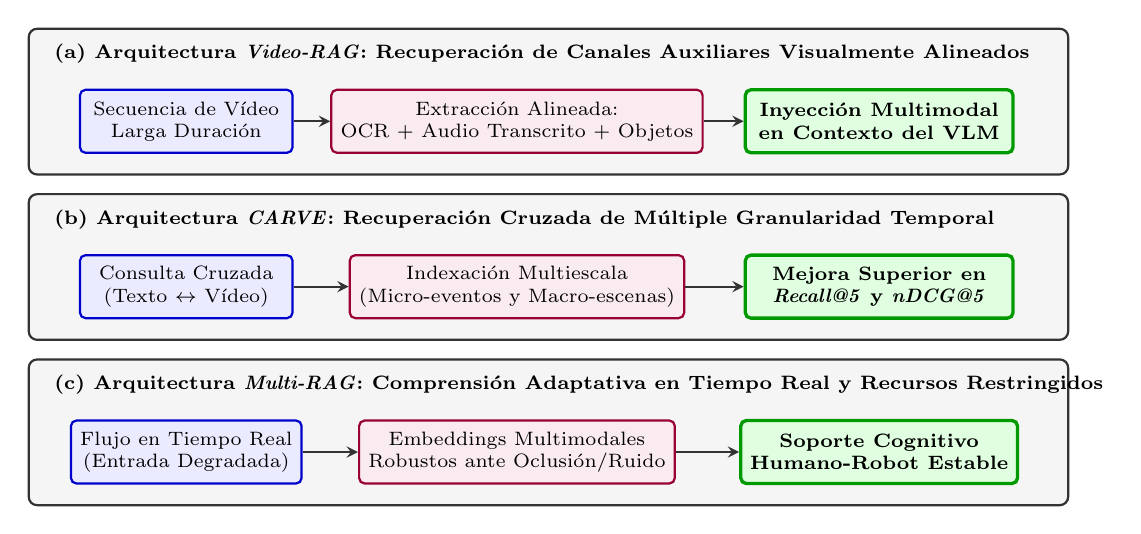
\begin{tikzpicture}[
    node distance=0.45cm and 0.6cm,
    archbox/.style={rectangle, draw=black!80, fill=gray!8, thick, minimum width=13.2cm, minimum height=1.85cm, rounded corners=3pt},
    innode/.style={rectangle, draw=blue!80!black, fill=blue!8, thick, minimum width=2.7cm, minimum height=0.8cm, align=center, font=\scriptsize, rounded corners=2pt},
    midnode/.style={rectangle, draw=purple!80!black, fill=purple!8, thick, minimum width=3.6cm, minimum height=0.8cm, align=center, font=\scriptsize, rounded corners=2pt},
    outnode/.style={rectangle, draw=green!60!black, fill=green!12, very thick, minimum width=3.4cm, minimum height=0.8cm, align=center, font=\scriptsize\bfseries, rounded corners=2pt},
    arrow/.style={-stealth, thick, draw=black!80}
]
% Video-RAG
\node[archbox] (b1) at (0, 4.2) {};
\node[font=\scriptsize\bfseries, anchor=north west] at (-6.4, 5.05) {(a) Arquitectura \textit{Video-RAG}: Recuperación de Canales Auxiliares Visualmente Alineados};
\node[innode] (v1_in) at (-4.6, 3.95) {Secuencia de Vídeo\\Larga Duración};
\node[midnode] (v1_mid) at (-0.4, 3.95) {Extracción Alineada:\\OCR + Audio Transcrito + Objetos};
\node[outnode] (v1_out) at (4.2, 3.95) {Inyección Multimodal\\en Contexto del VLM};
\draw[arrow] (v1_in) -- (v1_mid);
\draw[arrow] (v1_mid) -- (v1_out);

% CARVE
\node[archbox] (b2) at (0, 2.1) {};
\node[font=\scriptsize\bfseries, anchor=north west] at (-6.4, 2.95) {(b) Arquitectura \textit{CARVE}: Recuperación Cruzada de Múltiple Granularidad Temporal};
\node[innode] (v2_in) at (-4.6, 1.85) {Consulta Cruzada\\(Texto $\leftrightarrow$ Vídeo)};
\node[midnode] (v2_mid) at (-0.4, 1.85) {Indexación Multiescala\\(Micro-eventos y Macro-escenas)};
\node[outnode] (v2_out) at (4.2, 1.85) {Mejora Superior en\\\textit{Recall@5} y \textit{nDCG@5}};
\draw[arrow] (v2_in) -- (v2_mid);
\draw[arrow] (v2_mid) -- (v2_out);

% Multi-RAG
\node[archbox] (b3) at (0, 0.0) {};
\node[font=\scriptsize\bfseries, anchor=north west] at (-6.4, 0.85) {(c) Arquitectura \textit{Multi-RAG}: Comprensión Adaptativa en Tiempo Real y Recursos Restringidos};
\node[innode] (v3_in) at (-4.6, -0.25) {Flujo en Tiempo Real\\(Entrada Degradada)};
\node[midnode] (v3_mid) at (-0.4, -0.25) {Embeddings Multimodales\\Robustos ante Oclusión/Ruido};
\node[outnode] (v3_out) at (4.2, -0.25) {Soporte Cognitivo\\Humano-Robot Estable};
\draw[arrow] (v3_in) -- (v3_mid);
\draw[arrow] (v3_mid) -- (v3_out);
\end{tikzpicture}
\caption{Comparativa de tres arquitecturas representativas de sistemas RAG de vídeo en la literatura reciente: (a) alineación de metadatos auxiliares en \textit{Video-RAG}, (b) indexación multigranular en \textit{CARVE} y (c) inferencia adaptativa resiliente en \textit{Multi-RAG} \cite{video_rag2024, multi_rag2025}.} %[cite: 3, 5]
\label{fig:arquitecturas_videorag_carve_multirag}
\end{figure}

\subsubsection{Del Emparejamiento Semántico al Anclaje Causal Espaciotemporal (\textit{Temporal Grounding})}
\label{subsubsec:anclaje_causal_espaciotemporal}

El avance conceptual más profundo que caracteriza a la generación actual de sistemas Video RAG es el desplazamiento cualitativo desde el ``análisis temático'' hacia el verdadero \textbf{razonamiento y anclaje causal espaciotemporal (\textit{Temporal Grounding})} \cite{mixpeek_chunking, gemini_emb2_docs}. %[cite: 5, 6]
Los sistemas RAG tradicionales aplicados a multimedia se limitaban a responder preguntas resumiendo la temática general de un archivo (por ejemplo, devolver una síntesis genérica indicando que \textit{``el vídeo debate sobre economía''}). %[cite: 5]

Por el contrario, la convergencia de la fragmentación semántica adaptativa (\textit{Video-RAC}), los modelos de transcripción con alineación forzada (\textit{WhisperX}) y la diarización acústica de hablantes con modelos de \textit{embeddings} omnimodales permite que las arquitecturas contemporáneas formulen aserciones fundamentadas con precisión de milisegundos sobre la línea de tiempo \cite{video_rac2025, mixpeek_chunking}: %[cite: 5]

\begin{quote}
\textit{``Exactamente en el segmento 14:32, el segundo hablante señala el cuadrante superior derecho de la tabla, y el gráfico de barras indica un descenso de los ingresos, lo cual contradice el resumen textual proporcionado al inicio de la sesión''} \cite{mixpeek_chunking}. %[cite: 5]
\end{quote}

En este paradigma de \textit{grounding} temporal, el modelo cognitivo no inventa relaciones abstractas ni realiza aproximaciones difusas: se posiciona sobre un eje cronológico determinista $[t_{\text{inicio}}, t_{\text{fin}}]$ y discrimina el orden causal de los acontecimientos dentro de secuencias densas \cite{gemini_emb2_docs, mixpeek_chunking}. %[cite: 5, 6]
La Figura~\ref{fig:emparejamiento_vs_grounding_temporal} contrasta la salida de un sistema de emparejamiento temático clásico frente a un motor dotado de anclaje causal espaciotemporal. %[cite: 5, 6]

\begin{figure}[htbp]
\centering
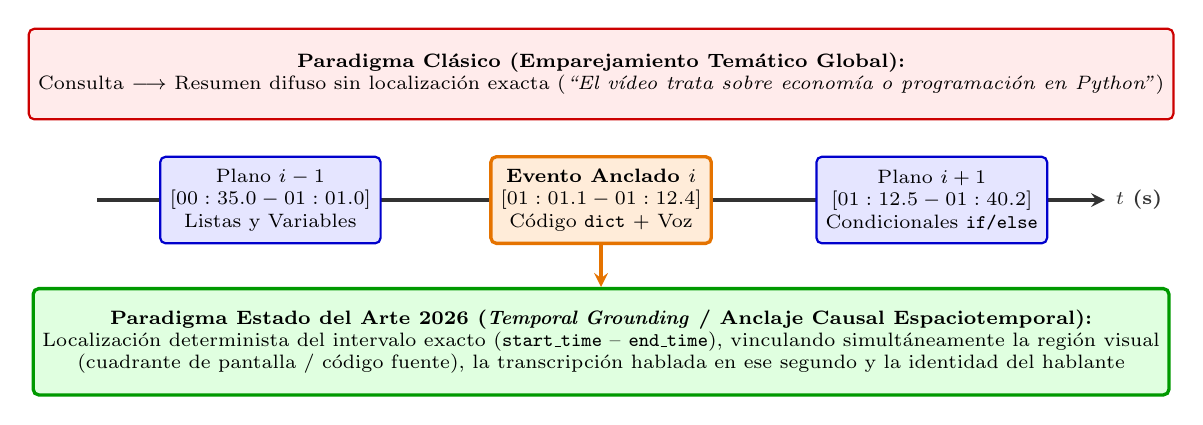
\begin{tikzpicture}[
    node distance=0.5cm and 0.7cm,
    oldbox/.style={rectangle, draw=red!80!black, fill=red!8, thick, minimum width=12.8cm, minimum height=1.15cm, align=center, font=\scriptsize, rounded corners=2pt},
    timebox/.style={rectangle, draw=blue!80!black, fill=blue!10, thick, minimum width=2.8cm, minimum height=1.1cm, align=center, font=\scriptsize, rounded corners=2pt},
    groundbox/.style={rectangle, draw=green!60!black, fill=green!12, very thick, minimum width=12.8cm, minimum height=1.35cm, align=center, font=\scriptsize, rounded corners=2pt},
    arrow/.style={-stealth, thick, draw=black!80}
]
% Paradigma Antiguo
\node[oldbox] (old) at (0, 2.3) {\textbf{Paradigma Clásico (Emparejamiento Temático Global):}\\
Consulta $\longrightarrow$ Resumen difuso sin localización exacta (\textit{``El vídeo trata sobre economía o programación en Python''})};

% Línea de tiempo determinista
\draw[-stealth, very thick, black!80] (-6.4, 0.7) -- (6.4, 0.7) node[right, font=\scriptsize\bfseries] {$t$ (s)};
\node[timebox] (c1) at (-4.2, 0.7) {Plano $i-1$\\$[00:35.0 - 01:01.0]$\\Listas y Variables};
\node[timebox, draw=orange!90!black, fill=orange!15, very thick] (c2) at (0.0, 0.7) {\textbf{Evento Anclado $i$}\\$[01:01.1 - 01:12.4]$\\Código \texttt{dict} + Voz};
\node[timebox] (c3) at (4.2, 0.7) {Plano $i+1$\\$[01:12.5 - 01:40.2]$\\Condicionales \texttt{if/else}};

% Paradigma Grounding Temporal
\node[groundbox] (new) at (0, -1.1) {\textbf{Paradigma Estado del Arte 2026 (\textit{Temporal Grounding} / Anclaje Causal Espaciotemporal):}\\
Localización determinista del intervalo exacto (\texttt{start\_time} -- \texttt{end\_time}), vinculando simultáneamente la región visual\\(cuadrante de pantalla / código fuente), la transcripción hablada en ese segundo y la identidad del hablante};

\draw[arrow, very thick, orange!90!black] (c2.south) -- (new.north);
\end{tikzpicture}
\caption{Contraste entre el emparejamiento temático tradicional y el Anclaje Causal Espaciotemporal (\textit{Temporal Grounding}), el cual proporciona trazabilidad determinista y auditable sobre la línea de tiempo del vídeo \cite{mixpeek_chunking, gemini_emb2_docs}.} %[cite: 5, 6]
\label{fig:emparejamiento_vs_grounding_temporal}
\end{figure}

Esta capacidad de anclaje milimétrico y judicialmente auditable habilita cinco dominios estratégicos de aplicación documentados en el proyecto \cite{gemini_emb2_docs}: %[cite: 5, 6]
\begin{enumerate}
    \item \textbf{Educación y Repositorios Académicos (RAG de Clases Grabadas):} Permite a un estudiante consultar \textit{``minuto donde el profesor explica la mitosis usando el diagrama en la pizarra''} o localizar el instante exacto en que un tutorial de programación explica cómo construir listas, diccionarios o condicionales \texttt{if/else}, razonando sobre la conjunción del audio y el código en pantalla. %[cite: 3, 6]
    \item \textbf{Auditoría de Seguridad y Videovigilancia:} Capacidad para inspeccionar cientos de horas de cámaras de seguridad sin supervisión humana mediante consultas en lenguaje natural como \textit{``coche rojo saltándose un semáforo a gran velocidad''} o \textit{``persona abandonando una mochila gris''}, recuperando las marcas de tiempo exactas. %[cite: 6]
    \item \textbf{Gestión de Archivos de Medios y \textit{Broadcasting}:} Localización instantánea en archivos históricos de televisión mediante búsquedas que combinan carga visual y entonación acústica, tales como \textit{``momentos de tensión en debates políticos''} o \textit{``personas llorando de alegría''}. %[cite: 6]
    \item \textbf{Análisis de Historiales Médicos y Diagnóstico Continuo:} Construcción de un perfil vectorial unificado que proyecta los informes clínicos en texto libre junto con las pruebas diagnósticas de imagen (radiografías, resonancias o ecografías) para encontrar casos clínicos equivalentes o auditar secuencias médicas. %[cite: 5, 6]
    \item \textbf{Comercio Electrónico y Búsqueda Visual Cruzada:} Recuperación de artículos específicos en catálogos multimedia a partir de una fotografía o una nota de voz descriptiva del usuario (\textit{``busco un sofá verde esmeralda de terciopelo con patas de madera''}). %[cite: 6]
\end{enumerate}

\subsubsection{Cuellos de Botella Perceptivos en la Verificación Visual: Resolución Espacial y Compresión JPEG}
\label{subsubsec:cuellos_botella_perceptivos_ocr}

Si bien la teoría de los modelos fundacionales multimodales postula la eliminación de los motores OCR tradicionales gracias a la lectura directa de parches visuales \cite{prajwal2025multimodal}, la experimentación empírica en sistemas reales revela que el \textbf{OCR implícito} de un modelo de visión-lenguaje es altamente sensible a las transformaciones de preprocesamiento de imagen aplicadas en el \textit{pipeline} de ingestión. %[cite: 3, 5]

En una arquitectura de búsqueda en dos etapas que utiliza \textit{Gemini Embedding 2} (vía Qdrant) para recuperar los fragmentos candidatos y emplea un modelo ligero secundario (\textit{Gemini 1.5 Flash Lite} o \textit{Gemini Flash 3.5}) como verificador visual para descartar falsos positivos, un ajuste agresivo de los hiperparámetros de codificación visual induce fallos críticos de falso rechazo (falsos negativos). %[cite: 3]

Durante las pruebas empíricas sobre el vídeo de validación \texttt{python\_tutorial.mp4} (\textit{``Python en 8 Minutos''}), al ejecutar la consulta \texttt{"Diccionarios"}, el motor vectorial recuperó en la quinta posición el intervalo temporal $01\text{:}01.1\text{ -- }01\text{:}40.2$ ($61,1\text{ s -- }100,2\text{ s}$). %[cite: 3]
Aunque la verdad terreno (\textit{ground truth}) del vídeo muestra explícitamente en pantalla entre los segundos $01\text{:}01.0$ y $01\text{:}03.0$ la sintaxis de un diccionario en Python (\texttt{dict \{"name": "Brais"\}}), el verificador visual descartó erróneamente el fragmento emitiendo el diagnóstico: \textit{``Descartado (Falso Positivo: 0\%) -- Análisis visual: El segmento cubre listas y variables, pero no muestra diccionarios''}. %[cite: 3]

La auditoría técnica de los parámetros de indexación demuestra que este fallo perceptivo responde a dos cuellos de botella en la codificación de los fotogramas clave antes de su envío a la API: %[cite: 3]
\begin{enumerate}
    \item \textbf{Resolución espacial destructiva (\texttt{resize\_width = 512}\text{ px}):} Redimensionar un videotutorial grabado en alta definición —donde el código fuente ocupa una fracción reducida del editor en pantalla— a un ancho máximo de $512$ píxeles reduce la altura de las tipografías a apenas unos pocos píxeles borrosos. %[cite: 3]
    Incluso manteniendo una calidad JPEG alta ($80$), a $512\text{ px}$ los caracteres de la palabra reservada \texttt{dict} y las llaves \texttt{\{\}} pierden su definición geométrica, impidiendo que tanto \textit{Gemini Embedding 2} como \textit{Gemini Flash} puedan leer la sintaxis. %[cite: 3]
    \item \textbf{Cuantización JPEG agresiva (\texttt{jpeg\_quality = 12} o \texttt{20}):} Cuando además de baja resolución se aplica un factor de calidad JPEG extremo ($12$ o $20$ en la escala $1\text{--}100$ de \texttt{cv2.imencode}), los macrobloques de la Transformada Discreta del Coseno (DCT) difuminan por completo los bordes de alto contraste del texto sobre el fondo del editor, convirtiendo el código en un artefacto ilegible. %[cite: 3]
\end{enumerate}

La Figura~\ref{fig:cuello_botella_ocr_implicito} esquematiza el mecanismo exacto por el cual la degradación de resolución y compresión induce alucinaciones de descarte en el verificador visual, así como los rangos de calibración óptimos. %[cite: 3]

\begin{figure}[htbp]
\centering
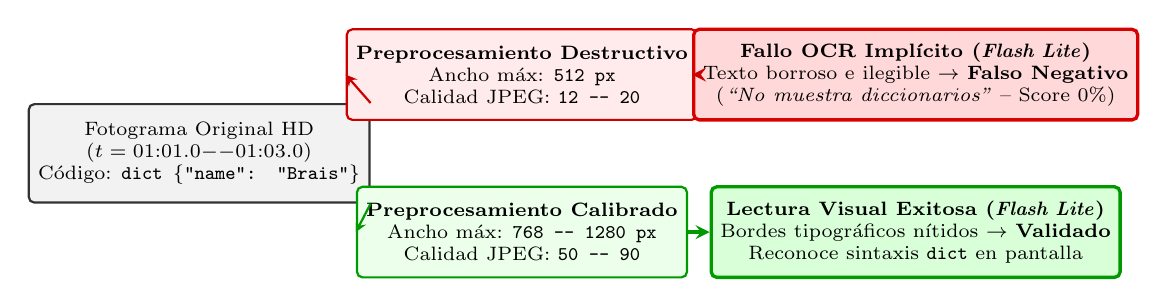
\begin{tikzpicture}[
    node distance=0.5cm and 0.65cm,
    srcbox/.style={rectangle, draw=black!80, fill=gray!10, thick, minimum width=2.8cm, minimum height=1.25cm, align=center, font=\scriptsize, rounded corners=2pt},
    badproc/.style={rectangle, draw=red!80!black, fill=red!8, thick, minimum width=3.4cm, minimum height=1.15cm, align=center, font=\scriptsize, rounded corners=2pt},
    goodproc/.style={rectangle, draw=green!60!black, fill=green!8, thick, minimum width=3.4cm, minimum height=1.15cm, align=center, font=\scriptsize, rounded corners=2pt},
    badout/.style={rectangle, draw=red!85!black, fill=red!15, very thick, minimum width=4.5cm, minimum height=1.15cm, align=center, font=\scriptsize, rounded corners=2pt},
    goodout/.style={rectangle, draw=green!60!black, fill=green!15, very thick, minimum width=4.5cm, minimum height=1.15cm, align=center, font=\scriptsize, rounded corners=2pt},
    arrow/.style={-stealth, thick, draw=black!80}
]
\node[srcbox] (frame) at (-5.2, 0.0) {Fotograma Original HD\\($t = 01\text{:}01.0\text{ -- }01\text{:}03.0$)\\Código: \texttt{dict \{"name": "Brais"\}}};

% Rama Superior: Degradación Crítica
\node[badproc] (b_enc) at (-1.1, 1.0) {\textbf{Preprocesamiento Destructivo}\\Ancho máx: \texttt{512 px}\\Calidad JPEG: \texttt{12 -- 20}};
\node[badout] (b_vlm) at (3.9, 1.0) {\textbf{Fallo OCR Implícito (\textit{Flash Lite})}\\Texto borroso e ilegible $\to$ \textbf{Falso Negativo}\\(\textit{``No muestra diccionarios''} -- Score 0\%)};

% Rama Inferior: Calibración Óptima
\node[goodproc] (g_enc) at (-1.1, -1.0) {\textbf{Preprocesamiento Calibrado}\\Ancho máx: \texttt{768 -- 1280 px}\\Calidad JPEG: \texttt{50 -- 90}};
\node[goodout] (g_vlm) at (3.9, -1.0) {\textbf{Lectura Visual Exitosa (\textit{Flash Lite})}\\Bordes tipográficos nítidos $\to$ \textbf{Validado}\\Reconoce sintaxis \texttt{dict} en pantalla};

\draw[arrow, red!80!black, thick] (frame.north east) -- (b_enc.west);
\draw[arrow, red!80!black, very thick] (b_enc.east) -- (b_vlm.west);
\draw[arrow, green!60!black, thick] (frame.south east) -- (g_enc.west);
\draw[arrow, green!60!black, very thick] (g_enc.east) -- (g_vlm.west);
\end{tikzpicture}
\caption{Diagnóstico del cuello de botella perceptivo en la etapa de verificación visual: el escalado a $512\text{ px}$ combinado con compresión JPEG agresiva ($12\text{--}20$) impide el OCR implícito de sintaxis de programación en pantalla, mientras que elevar \texttt{resize\_width} al rango $768\text{--}1280\text{ px}$ y la calidad JPEG a $50\text{--}90$ restaura la detección sin disparar el consumo de cuota.} %[cite: 3]
\label{fig:cuello_botella_ocr_implicito}
\end{figure}

\subsubsection{Dilución Semántica en Fragmentos de Larga Duración y Muestreo Estático de Fotogramas}
\label{subsubsec:dilucion_semantica_muestreo}

El segundo fenómeno crítico identificado durante la validación del sistema es el problema de la \textbf{dilución semántica y pérdida de fotogramas clave} en fragmentos de larga duración. %[cite: 3]
En vídeos con un fondo visual altamente estático —tales como clases grabadas, presentaciones de diapositivas o tutoriales de código donde el entorno gráfico del editor permanece inalterado y únicamente cambian unas pocas líneas de texto—, el índice de similitud estructural (SSIM) entre fotogramas consecutivos se mantiene elevado durante largos periodos. %[cite: 3]

Cuando el umbral de corte SSIM se configura en un valor demasiado permisivo (\texttt{threshold = 0.08}) o incluso en un valor moderado (\texttt{threshold = 0.60}) sin imponer una duración máxima de plano, el algoritmo agrupa secuencias extensas en un único \texttt{VideoChunk} —como el citado fragmento \#5 de $39,1$ segundos de duración ($01\text{:}01.1\text{ -- }01\text{:}40.2$)—. %[cite: 3]
A una cadencia estándar de $f_{\text{fps}} = 30$ fotogramas por segundo, un fragmento de $\Delta T = 39,1\text{ s}$ contiene un total de $N_{\text{total}} = \Delta T \times f_{\text{fps}} \approx 1.173$ fotogramas. %[cite: 3]
Dado que la función \texttt{extract\_key\_frames} selecciona un número estático de $k = 3$ fotogramas por fragmento (inicial, final y máxima entropía), la fracción de cobertura temporal cae drásticamente, provocando dos efectos adversos: %[cite: 3]
\begin{itemize}
    \item \textbf{Omisión por submuestreo (\textit{Keyframe Miss}):} Si el evento buscado (la escritura de \texttt{dict \{"name": "Brais"\}}) ocurre entre los segundos $01\text{:}01.0$ y $01\text{:}03.0$, pero el fotograma de máxima entropía global de esos $39,1$ segundos recae en el segundo $01\text{:}25.0$ (donde la pantalla está más llena de código de listas o variables), ninguno de los $3$ fotogramas enviados a la API contendrá el diccionario. %[cite: 3]
    \item \textbf{Dilución del vector agregado en el espacio latente:} Al mezclar en un único \texttt{VideoChunk} casi $40$ segundos que abarcan múltiples subtemas distintos (variables, listas y diccionarios), el vector resultante en \textit{Gemini Embedding 2} promedia todas esas temáticas, perdiendo especificidad direccional frente a consultas puntuales. %[cite: 3]
\end{itemize}

La Figura~\ref{fig:dilucion_semantica_chunks_largos} ilustra gráficamente cómo se produce esta pérdida por muestreo en un \textit{chunk} gigante y cómo la corrigen las estrategias de acotación temporal o muestreo dinámico. %[cite: 3]

\begin{figure}[htbp]
\centering
\begin{tikzpicture}[scale=0.95]
% Caso A: Chunk Gigante (39.1s) con pérdida de fotograma clave
\node[font=\scriptsize\bfseries, anchor=west] at (0, 2.5) {(a) Fragmento Masivo sin Límite Superior ($\Delta T = 39,1\text{ s}$, Umbral SSIM $= 0,08 / 0,60$ en vídeo estático):};
\draw[fill=red!8, draw=red!80!black, thick, rounded corners=2pt] (0, 1.3) rectangle (12.6, 2.2);
\node[font=\scriptsize, red!80!black] at (6.3, 1.75) {\texttt{VideoChunk \#5} ($01\text{:}01.1 \longrightarrow 01\text{:}40.2$) --- Mezcla Variables, Listas y Diccionarios (Dilución Semántica)};

% Zona donde ocurre realmente el diccionario
\draw[fill=yellow!35, draw=orange!90!black, very thick] (0.2, 1.3) rectangle (1.3, 2.2);
\node[above, font=\tiny\bfseries, orange!90!black] at (0.75, 2.2) {Evento \texttt{dict} ($01\text{:}03$)};

% Los 3 fotogramas muestreados (F1, F_entropia, F3) que fallan el evento
\filldraw[blue!80!black] (0.05, 1.75) circle (3pt) node[below=4pt, font=\tiny\bfseries] {$F_{\text{ini}}$};
\filldraw[blue!80!black] (7.8, 1.75) circle (3pt) node[below=4pt, font=\tiny\bfseries] {$F_{\text{entropía}}$ (Listas)};
\filldraw[blue!80!black] (12.55, 1.75) circle (3pt) node[below=4pt, font=\tiny\bfseries] {$F_{\text{fin}}$};

% Caso B: Corrección mediante max_shot_frames (10-15s) o Muestreo Proporcional
\node[font=\scriptsize\bfseries, anchor=west] at (0, 0.35) {(b) Solución Arquitectónica: Corte Forzado por Duración Máxima (\texttt{max\_shot\_frames} $\approx 10\text{--}15\text{ s}$) o Muestreo Dinámico:};
\draw[fill=green!12, draw=green!60!black, very thick, rounded corners=2pt] (0, -0.8) rectangle (3.1, 0.05);
\node[font=\tiny\bfseries, green!50!black] at (1.55, -0.37) {Sub-Chunk 5a ($01\text{:}01\text{--}01\text{:}11$): \textbf{Captura \texttt{dict}}};

\draw[fill=gray!12, draw=black!70, thick, rounded corners=2pt] (3.2, -0.8) rectangle (6.3, 0.05);
\node[font=\tiny] at (4.75, -0.37) {Sub-Chunk 5b ($01\text{:}11\text{--}01\text{:}21$)};

\draw[fill=gray!12, draw=black!70, thick, rounded corners=2pt] (6.4, -0.8) rectangle (9.5, 0.05);
\node[font=\tiny] at (7.95, -0.37) {Sub-Chunk 5c ($01\text{:}21\text{--}01\text{:}31$)};

\draw[fill=gray!12, draw=black!70, thick, rounded corners=2pt] (9.6, -0.8) rectangle (12.6, 0.05);
\node[font=\tiny] at (11.1, -0.37) {Sub-Chunk 5d ($01\text{:}31\text{--}01\text{:}40$)};
\end{tikzpicture}
\caption{Mecanismo de dilución semántica y pérdida de fotogramas clave en vídeos con baja variación visual: (a) un fragmento de casi $40\text{ s}$ muestreado con solo $3$ fotogramas omite el instante en que aparece el diccionario y mezcla múltiples temas; (b) la imposición de un límite superior (\texttt{max\_shot\_frames} de $10\text{--}15\text{ s}$) o la extracción proporcional (un fotograma extra cada $5\text{ s}$) garantiza la cohesión semántica.} %[cite: 3]
\label{fig:dilucion_semantica_chunks_largos}
\end{figure}

El Cuadro~\ref{tab:diagnostico_parametros_visuales} resume la comparativa técnica entre las configuraciones defectuosas analizadas durante la depuración y los rangos corregidos necesarios para preservar tanto la legibilidad del texto en pantalla como la granularidad temporal de los fragmentos. %[cite: 3]

\begin{table}[htbp]
\centering
\caption{Diagnóstico empírico de parámetros de preprocesamiento visual y temporal en sistemas Video RAG con verificación secundaria (\textit{Gemini Embedding 2} + \textit{Gemini Flash}) \cite{gemini_emb2_docs}.} %[cite: 3]
\label{tab:diagnostico_parametros_visuales}
\begin{tabular}{llll}
\hline
\textbf{Parámetro del Pipeline} & \textbf{Config. Defectuosa} & \textbf{Efecto Patológico en el RAG} & \textbf{Configuración Óptima Calibrada} \\
\hline
Ancho máx. (\texttt{resize\_width}) & $512\text{ px}$ & Texto/código ilegible (fallo OCR implícito) & $768\text{ px}$ a $1.280\text{ px}$ (nitidez tipográfica) \\
Calidad JPEG (\texttt{jpeg\_quality}) & $12$ a $20$ & Artefactos de bloque borran la sintaxis & $50\text{--}70$ (equilibrio) o $80\text{--}90$ (alta) \\
Umbral SSIM (\texttt{threshold}) & $0,08$ (o $0,60$ estático) & Chunks gigantes ($\sim 40\text{ s}$); dilución vectorial & $0,50\text{--}0,80$ + cota superior temporal \\
Duración máx. (\texttt{max\_shot\_frames}) & Sin límite ($\infty$) & Pérdida de evento al extraer solo 3 frames & Corte forzado cada $10\text{--}15\text{ s}$ máx. \\
Muestreo (\texttt{extract\_key\_frames}) & Fijo ($3$ frames/chunk) & Submuestreo severo en planos largos & $3$ frames (cortos) o $+1$ frame cada $5\text{ s}$ \\
\hline
\end{tabular}
\end{table}

Estos resultados demuestran que la eficacia de un modelo fundacional omnimodal no depende únicamente de su capacidad neuronal en la nube, sino de que la canalización local de visión por computador preserve la resolución tipográfica suficiente y acote la duración temporal de cada fragmento antes de la vectorización. %[cite: 3]

% Bloque 2.6: Estrategias de Fragmentación (Chunking) y Alineación Temporal (Págs. 25-27)
% =============================================================================
% CAPÍTULO 2 - BLOQUE 2.6: ESTRATEGIAS AVANZADAS DE FRAGMENTACIÓN (CHUNKING),
% FORMULACIÓN GAUSSIANA SSIM, SELECCIÓN POR ENTROPÍA Y ALINEACIÓN AUDITIVA
% =============================================================================

\subsection{Estrategias Avanzadas de Fragmentación (\textit{Chunking}) y Alineación Temporal}
\label{subsec:chunking_alineacion}

\subsubsection{Obsolescencia de la Partición Fija, Detección de Planos y Agrupación de Escenas}
\label{subsubsec:obsolescencia_particion_fija}

El rendimiento, la precisión de recuperación y la viabilidad técnica de cualquier arquitectura de vectorización multimodal recaen, fundamentalmente, sobre su estrategia de partición de datos o \textit{chunking} \cite{adaptive_chunking2026, multi_rag2025}. %
Indexar las pistas de audio, los subtítulos y las secuencias de fotogramas de vídeo de forma desincronizada o mediante divisiones temporales arbitrarias destruye por completo la cohesión semántica y cronológica del documento multimedia \cite{mixpeek_chunking}. %[cite: 5]

La metodología de fragmentación más elemental —consistente en cortar un archivo de vídeo en intervalos regulares y rígidos, por ejemplo, cada $5$ o $10$ segundos— constituye un enfoque obsoleto en el estado del arte de 2026 \cite{video_rac2025, mixpeek_chunking}. %[cite: 3, 5]
Aplicar una rejilla temporal ciega produce invariablemente cortes abruptos en mitad de una oración hablada, interrumpe un cambio de plano cinematográfico o divide en dos fragmentos inconexos la transición de una diapositiva académica o la escritura de un bloque de código \cite{video_rac2025, mixpeek_chunking}. %[cite: 3, 5]
Forzar posteriormente al modelo de \textit{embeddings} o al modelo generativo a interpretar fragmentos visuales mutilados introduce un ruido contextual severo que degrada las métricas de relevancia y fidelidad \cite{video_rac2025}. %[cite: 5]

Para erradicar esta fragmentación destructiva, las arquitecturas contemporáneas aplican algoritmos de \textbf{detección de límites de plano (\textit{shot boundary detection})} acoplados a procesamiento paralelo profundo \cite{mixpeek_chunking}. %[cite: 3, 5]
Estos algoritmos evalúan fotograma a fotograma la continuidad visual midiendo bien la divergencia de histogramas en espacios de color robustos ante variaciones de iluminación —como el espacio HSV (\textit{Hue, Saturation, Value}), donde un parpadeo de cámara afecta al canal de valor pero no altera el matiz cromático—, o bien la similitud estructural (SSIM) entre fotogramas secuenciales, garantizando que cada \textit{chunk} represente una unidad narrativa o visualmente coherente \cite{mixpeek_chunking, video_rac2025}. %[cite: 3, 5]

Por otra parte, cuando el vídeo presenta cortes de cámara muy rápidos y la granularidad del plano resultante es excesivamente fina, la literatura incorpora técnicas de \textbf{agrupación de escenas (\textit{scene grouping})} \cite{mixpeek_chunking}. %[cite: 5]
Este procedimiento fusiona planos consecutivos cuyas representaciones vectoriales preliminares superan un umbral de similitud predefinido, condensando múltiples micro-planos en intervalos temporales más largos y semánticamente estables antes de su indexación definitiva \cite{mixpeek_chunking}. %[cite: 5]

La Figura~\ref{fig:fixed_vs_adaptive_videorac} contrasta el efecto destructivo de la partición por intervalos fijos frente a la preservación de unidades narrativas mediante detección adaptativa de límites de plano y agrupación de escenas. %[cite: 3, 5]

\begin{figure}[htbp]
\centering
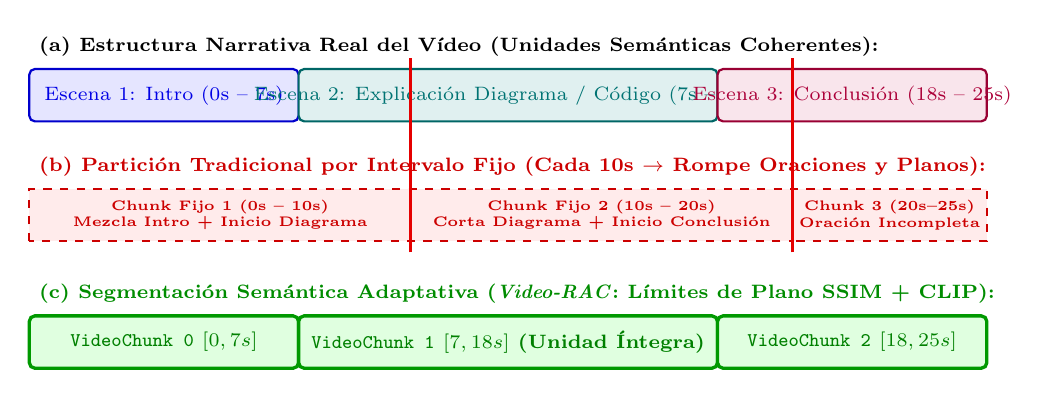
\begin{tikzpicture}[scale=0.95]
% Flujo Real de Eventos en el Vídeo
\node[font=\scriptsize\bfseries, anchor=west] at (0, 3.3) {(a) Estructura Narrativa Real del Vídeo (Unidades Semánticas Coherentes):};
\draw[fill=blue!10, draw=blue!80!black, thick, rounded corners=2pt] (0, 2.3) rectangle (3.6, 3.0);
\node[font=\scriptsize, blue!90!black] at (1.8, 2.65) {Escena 1: Intro (0s -- 7s)};

\draw[fill=teal!12, draw=teal!80!black, thick, rounded corners=2pt] (3.6, 2.3) rectangle (9.2, 3.0);
\node[font=\scriptsize, teal!90!black] at (6.4, 2.65) {Escena 2: Explicación Diagrama / Código (7s -- 18s)};

\draw[fill=purple!10, draw=purple!80!black, thick, rounded corners=2pt] (9.2, 2.3) rectangle (12.8, 3.0);
\node[font=\scriptsize, purple!90!black] at (11.0, 2.65) {Escena 3: Conclusión (18s -- 25s)};

% Partición Fija (Obsoleta)
\node[font=\scriptsize\bfseries, red!80!black, anchor=west] at (0, 1.7) {(b) Partición Tradicional por Intervalo Fijo (Cada 10s $\to$ Rompe Oraciones y Planos):};
\draw[fill=red!8, draw=red!80!black, thick, dashed] (0, 0.7) rectangle (5.1, 1.4);
\node[font=\tiny\bfseries, red!80!black, align=center] at (2.55, 1.05) {Chunk Fijo 1 (0s -- 10s)\\Mezcla Intro + Inicio Diagrama};

\draw[fill=red!8, draw=red!80!black, thick, dashed] (5.1, 0.7) rectangle (10.2, 1.4);
\node[font=\tiny\bfseries, red!80!black, align=center] at (7.65, 1.05) {Chunk Fijo 2 (10s -- 20s)\\Corta Diagrama + Inicio Conclusión};

\draw[fill=red!8, draw=red!80!black, thick, dashed] (10.2, 0.7) rectangle (12.8, 1.4);
\node[font=\tiny\bfseries, red!80!black, align=center] at (11.5, 1.05) {Chunk 3 (20s--25s)\\Oración Incompleta};

% Líneas de corte erróneas
\draw[very thick, red!90!black] (5.1, 0.55) -- (5.1, 3.15);
\draw[very thick, red!90!black] (10.2, 0.55) -- (10.2, 3.15);

% Segmentación Semántica Adaptativa (Video-RAC)
\node[font=\scriptsize\bfseries, green!55!black, anchor=west] at (0, 0.0) {(c) Segmentación Semántica Adaptativa (\textit{Video-RAC}: Límites de Plano SSIM + CLIP):};
\draw[fill=green!12, draw=green!60!black, very thick, rounded corners=2pt] (0, -1.0) rectangle (3.6, -0.3);
\node[font=\scriptsize\bfseries, green!50!black] at (1.8, -0.65) {\texttt{VideoChunk 0} $[0, 7\text{s}]$};

\draw[fill=green!12, draw=green!60!black, very thick, rounded corners=2pt] (3.6, -1.0) rectangle (9.2, -0.3);
\node[font=\scriptsize\bfseries, green!50!black] at (6.4, -0.65) {\texttt{VideoChunk 1} $[7, 18\text{s}]$ (Unidad Íntegra)};

\draw[fill=green!12, draw=green!60!black, very thick, rounded corners=2pt] (9.2, -1.0) rectangle (12.8, -0.3);
\node[font=\scriptsize\bfseries, green!50!black] at (11.0, -0.65) {\texttt{VideoChunk 2} $[18, 25\text{s}]$};
\end{tikzpicture}
\caption{Comparativa estructural entre (b) la división arbitraria en intervalos fijos, que introduce ruido contextual al cortar escenas y oraciones a la mitad, y (c) la segmentación semántica adaptativa (\textit{Video-RAC}), que alinea exactamente los límites de cada \texttt{VideoChunk} con las transiciones reales del contenido \cite{video_rac2025, mixpeek_chunking}.} %[cite: 3, 5]
\label{fig:fixed_vs_adaptive_videorac}
\end{figure}

\subsubsection{Metodología Híbrida \textit{Video-RAC} y Formulación Matemática del SSIM Gaussiano}
\label{subsubsec:metodologia_videorac_ssim}

Dentro del ámbito de los vídeos educativos, académicos y tutoriales técnicos, la arquitectura \textbf{Video-RAC (\textit{Retrieval Adaptive Chunking})} se ha consolidado como el estándar metodológico de referencia \cite{video_rac2025}. %[cite: 3, 5]
\textit{Video-RAC} abandona las particiones estáticas en favor de un criterio híbrido que evalúa cada transición temporal combinando la similitud del coseno de \textit{embeddings} visuales ligeros generados por CLIP con el Índice de Similitud Estructural (SSIM) \cite{video_rac2025}. %[cite: 3, 5]

Específicamente, la formulación teórica de \textit{Video-RAC} emplea el modelo \texttt{openai/clip-vit-base-patch32} para extraer representaciones rápidas de los fotogramas consecutivos $F_t$ y $F_{t+1}$, ponderando su similitud semántica con la similitud estructural mediante un factor de balance $\alpha = 0,6$ \cite{video_rac2025}: %[cite: 5]

\begin{equation}
S_{\text{híbrida}}(F_t, F_{t+1}) = \alpha \cdot \cos\!\left(\mathbf{e}_{\text{CLIP}}(F_t), \, \mathbf{e}_{\text{CLIP}}(F_{t+1})\right) + (1 - \alpha) \cdot \text{SSIM}(F_t, F_{t+1})
\label{eq:videorac_hibrido}
\end{equation} %[cite: 5]

Los hiperparámetros canónicos reportados en la literatura para determinar dónde concluye una unidad semántica y comienza la siguiente estipulan un factor de balance $\alpha = 0,6$, un umbral de similitud de \textit{embeddings} CLIP de $\tau_{\text{CLIP}} = 0,85$ y un umbral estructural de $\tau_{\text{SSIM}} = 0,80$ \cite{video_rac2025}. %[cite: 5]

En implementaciones de producción optimizadas para ejecutarse localmente en CPU sin requerir la carga de pesos adicionales de CLIP durante el preprocesamiento (tal y como se implementa en el módulo \texttt{src/processing/video\_chunker.py}), la detección de límites de plano se resuelve directamente mediante la formulación matemática exacta del \textbf{Índice de Similitud Estructural (SSIM)} con ventana Gaussiana en OpenCV. %[cite: 3]
Dados dos fotogramas consecutivos convertidos a escala de grises y redimensionados a un ancho de análisis rápido (\texttt{resize\_width = 160} píxeles para la fase de corte), representados como matrices en coma flotante de doble precisión $a, b \in \mathbb{R}^{H \times W}$ (\texttt{np.float64}), el algoritmo aplica un filtro de desenfoque Gaussiano bidimensional \texttt{cv2.GaussianBlur} con tamaño de núcleo impar $K \times K$ (\texttt{window\_size = 7}) y desviación estándar $\sigma = 1,5$ para obtener las medias locales $\mu_a, \mu_b$: %[cite: 3]

\begin{equation}
\mu_a = G_{K \times K, \, \sigma=1.5} * a, \qquad \mu_b = G_{K \times K, \, \sigma=1.5} * b
\label{eq:ssim_medias_locales}
\end{equation} %[cite: 3]

A partir de los cuadrados de las medias ($\mu_a^2, \mu_b^2$) y de su producto cruzado ($\mu_{ab} = \mu_a \mu_b$), las varianzas locales $\sigma_a^2, \sigma_b^2$ y la covarianza cruzada local $\sigma_{ab}$ se calculan matricialmente mediante convolución Gaussiana como: %[cite: 3]

\begin{equation}
\sigma_a^2 = \left(G_{K \times K, \, \sigma=1.5} * (a \odot a)\right) - \mu_a^2, \quad
\sigma_b^2 = \left(G_{K \times K, \, \sigma=1.5} * (b \odot b)\right) - \mu_b^2, \quad
\sigma_{ab} = \left(G_{K \times K, \, \sigma=1.5} * (a \odot b)\right) - \mu_{ab}
\label{eq:ssim_varianzas_covarianza}
\end{equation} %[cite: 3]

donde $\odot$ denota el producto elemento a elemento (\textit{Hadamard product}). %[cite: 3]
Con estas matrices estadísticas e introduciendo las constantes de estabilidad numérica para un rango dinámico de 8 bits ($L = 255$), definidas como $C_1 = (0,01 \times 255)^2 = 6,5025$ y $C_2 = (0,03 \times 255)^2 = 58,5225$, el mapa espacial SSIM y su escalar medio resultante en el rango $[-1, 1]$ vienen dados por: %[cite: 3]

\begin{equation}
\text{SSIM}_{\text{map}}(a, b) = \frac{(2\mu_{ab} + C_1)(2\sigma_{ab} + C_2)}{(\mu_a^2 + \mu_b^2 + C_1)(\sigma_a^2 + \sigma_b^2 + C_2)}, \qquad
\overline{\text{SSIM}}(a, b) = \frac{1}{H \cdot W} \sum_{y=1}^{H} \sum_{x=1}^{W} \text{SSIM}_{\text{map}}(y, x)
\label{eq:ssim_mapa_y_media}
\end{equation} %[cite: 3]

Cuando el valor escalar $\overline{\text{SSIM}}(a, b)$ cae por debajo del umbral configurado (\texttt{threshold}, calibrado entre $0,50$ y $0,80$) y el número de fotogramas acumulados desde el corte anterior iguala o supera el mínimo permitido (\texttt{min\_shot\_frames = 12} a $45$ fotogramas para filtrar destellos luminosos espurios), la función \texttt{detect\_shot\_boundaries} consolida e instancia un objeto inmutable \texttt{VideoChunk(index, start\_frame, end\_frame, start\_time, end\_time)}. %[cite: 3]

La Figura~\ref{fig:pipeline_ssim_opencv} detalla este flujo de cálculo matricial implementado en \texttt{compute\_ssim} y \texttt{detect\_shot\_boundaries}. %[cite: 3]

\begin{figure}[htbp]
\centering
\begin{tikzpicture}[
    node distance=0.45cm and 0.65cm,
    matbox/.style={rectangle, draw=black!80, fill=gray!10, thick, minimum width=2.7cm, minimum height=0.95cm, align=center, font=\scriptsize, rounded corners=2pt},
    blurbox/.style={rectangle, draw=blue!80!black, fill=blue!8, thick, minimum width=3.2cm, minimum height=1.1cm, align=center, font=\scriptsize, rounded corners=2pt},
    mapnode/.style={rectangle, draw=purple!80!black, fill=purple!8, thick, minimum width=3.3cm, minimum height=1.1cm, align=center, font=\scriptsize, rounded corners=2pt},
    decnode/.style={diamond, aspect=2.1, draw=orange!85!black, fill=orange!12, very thick, minimum width=2.8cm, minimum height=1.1cm, align=center, font=\scriptsize\bfseries},
    chunkbox/.style={rectangle, draw=green!60!black, fill=green!12, very thick, minimum width=2.9cm, minimum height=1.1cm, align=center, font=\scriptsize\bfseries, rounded corners=2pt},
    arrow/.style={-stealth, thick, draw=black!80}
]
\node[matbox] (frames) at (-5.3, 0.0) {Par Consecutivo\\$F_{t-1}, F_t$ (Grises)\\ \texttt{float64} ($160\text{ px}$)};

\node[blurbox] (gauss) at (-1.8, 0.0) {\texttt{cv2.GaussianBlur}\\Núcleo $7\times 7, \, \sigma = 1,5$\\$\mu_a, \mu_b, \sigma_a^2, \sigma_b^2, \sigma_{ab}$};

\node[mapnode] (ssim) at (1.9, 0.0) {Mapa $\text{SSIM}_{\text{map}}$\\($C_1, C_2$ con $L=255$)\\Media: \texttt{ssim\_map.mean()}};

\node[decnode] (cut) at (1.9, -2.0) {¿$\overline{\text{SSIM}} < \tau$\\y $\Delta f \ge f_{\min}$?};

\node[chunkbox] (out) at (5.6, -2.0) {Emite \texttt{VideoChunk}\\(\texttt{start\_frame}, \texttt{end\_frame},\\ \texttt{start\_time}, \texttt{end\_time})};

\node[matbox, minimum width=2.7cm] (cont) at (-2.1, -2.0) {Continúa Plano Actual\\Acumula Fotograma $F_t$};

\draw[arrow] (frames) -- (gauss);
\draw[arrow] (gauss) -- (ssim);
\draw[arrow] (ssim) -- (cut);
\draw[arrow, draw=green!60!black] (cut) -- node[above, font=\scriptsize\bfseries, green!60!black] {Sí (Corte)} (out);
\draw[arrow, draw=blue!80!black] (cut) -- node[above, font=\scriptsize\bfseries, blue!80!black] {No} (cont);
\end{tikzpicture}
\caption{Flujo algorítmico del cálculo del Índice de Similitud Estructural (SSIM) mediante filtrado Gaussiano en OpenCV (\texttt{compute\_ssim}) y criterio de consolidación de objetos \texttt{VideoChunk} en \texttt{detect\_shot\_boundaries}.} %[cite: 3]
\label{fig:pipeline_ssim_opencv}
\end{figure}

\subsubsection{Selección de Fotogramas Clave mediante Entropía Matemática de Shannon}
\label{subsubsec:seleccion_entropia_shannon}

Una vez que el vídeo ha sido particionado en unidades semánticamente coherentes (\texttt{VideoChunk}), enviar la totalidad de los fotogramas de cada fragmento (a razón de $30$ o $60$ fotogramas por segundo) hacia la API del modelo de \textit{embeddings} resultaría computacional y económicamente inviable \cite{video_rac2025, gemini_emb2_docs}. %[cite: 3]
Para comprimir el volumen visual sin perder el contenido informativo del plano, la metodología \textit{Video-RAC} establece una estrategia de \textbf{selección de fotogramas por entropía} implementada en la función \texttt{extract\_key\_frames} \cite{video_rac2025}. %[cite: 3]

Para cada objeto \texttt{VideoChunk} delimitado entre los índices de fotograma $[f_{\text{ini}}, f_{\text{fin}}]$, el algoritmo selecciona exactamente tres fotogramas representativos ordenados cronológicamente \cite{video_rac2025}: %[cite: 3]
\begin{enumerate}
    \item \textbf{Fotograma Inicial ($F_{f_{\text{ini}}}$):} Captura el estado visual de partida del evento al abrirse el plano. %[cite: 3]
    \item \textbf{Fotograma Intermedio de Máxima Entropía ($F_{f^*}$):} De entre los fotogramas interiores $t \in (f_{\text{ini}}, f_{\text{fin}})$ (evaluados de forma exhaustiva o mediante un paso de muestreo \texttt{entropy\_step}), se selecciona aquel que maximiza la \textbf{Entropía de Información de Shannon} $H(F_t)$, la cual cuantifica la riqueza y densidad de detalle visual (por ejemplo, el instante en que un diagrama o bloque de código está completamente desplegado en pantalla y no oculto o en transición). %[cite: 3]
    \item \textbf{Fotograma Final ($F_{f_{\text{fin}}}$):} Registra el estado consolidado del plano justo antes del corte hacia la siguiente escena. %[cite: 3]
\end{enumerate}

Matemáticamente, para calcular la entropía de Shannon de un fotograma candidato $F_t$ convertido a escala de grises con $L = 256$ niveles de intensidad ($i \in \{0, 1, \dots, 255\}$), se obtiene primero su histograma de frecuencias absolutas $h(i)$ mediante \texttt{cv2.calcHist} y se normaliza por el número total de píxeles $N_{\text{pix}} = H \times W$ para obtener la distribución de probabilidad discreta $p_i = h(i) / N_{\text{pix}}$: %[cite: 3]

\begin{equation}
H(F_t) = -\sum_{\substack{i=0 \\ p_i > 0}}^{255} p_i \log_2(p_i), \qquad f^* = \arg\max_{t \in (f_{\text{ini}}, \, f_{\text{fin}})} H(F_t)
\label{eq:entropia_shannon_keyframe}
\end{equation} %[cite: 3]

La Figura~\ref{fig:seleccion_entropia_shannon} ilustra la evolución de la curva de entropía $H(F_t)$ dentro de los límites de un \texttt{VideoChunk} y la extracción de la terna de matrices NumPy que alimenta al vectorizador multimodal. %[cite: 3]

\begin{figure}[htbp]
\centering
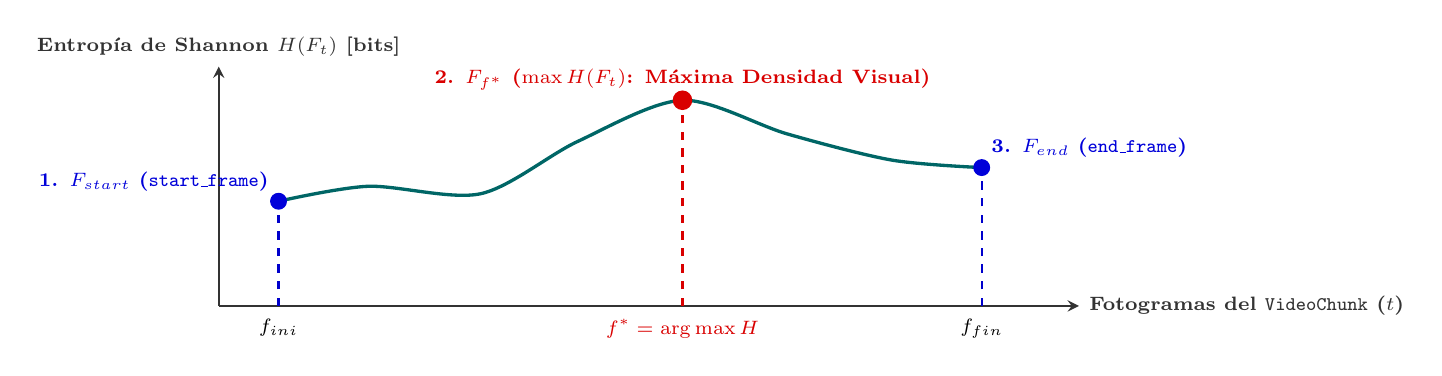
\begin{tikzpicture}[scale=0.95]
% Ejes de la gráfica de entropía
\draw[-stealth, thick, black!80] (0,0) -- (11.5,0) node[right, font=\scriptsize\bfseries] {Fotogramas del \texttt{VideoChunk} ($t$)};
\draw[-stealth, thick, black!80] (0,0) -- (0,3.2) node[above, font=\scriptsize\bfseries] {Entropía de Shannon $H(F_t)$ [bits]};

% Líneas de inicio, máximo y fin
\draw[dashed, blue!80!black, thick] (0.8, 0) -- (0.8, 1.4);
\draw[dashed, red!85!black, very thick] (6.2, 0) -- (6.2, 2.75);
\draw[dashed, blue!80!black, thick] (10.2, 0) -- (10.2, 1.85);

% Curva de entropía simulada dentro del chunk
\draw[very thick, teal!80!black] plot [smooth] coordinates {
    (0.8, 1.4) (2.0, 1.6) (3.5, 1.5) (4.8, 2.2) (6.2, 2.75) (7.6, 2.3) (9.0, 1.95) (10.2, 1.85)
};

% Puntos seleccionados
\filldraw[blue!85!black] (0.8, 1.4) circle (3pt) node[above left, font=\scriptsize\bfseries] {1. $F_{\text{start}}$ (\texttt{start\_frame})};
\filldraw[red!85!black] (6.2, 2.75) circle (3.5pt) node[above, font=\scriptsize\bfseries] {2. $F_{f^*}$ ($\max H(F_t)$: Máxima Densidad Visual)};
\filldraw[blue!85!black] (10.2, 1.85) circle (3pt) node[above right, font=\scriptsize\bfseries] {3. $F_{\text{end}}$ (\texttt{end\_frame})};

% Etiquetas en el eje X
\node[below, font=\scriptsize] at (0.8, -0.05) {$f_{\text{ini}}$};
\node[below, font=\scriptsize\bfseries, red!85!black] at (6.2, -0.05) {$f^* = \arg\max H$};
\node[below, font=\scriptsize] at (10.2, -0.05) {$f_{\text{fin}}$};
\end{tikzpicture}
\caption{Selección de fotogramas clave basada en Entropía de Shannon (\texttt{extract\_key\_frames}) según la metodología \textit{Video-RAC}: extracción del fotograma inicial, el fotograma final y el fotograma intermedio que maximiza la densidad de información visual $H(F_t)$ \cite{video_rac2025}.} %[cite: 3]
\label{fig:seleccion_entropia_shannon}
\end{figure}

\subsubsection{Alineación Forzada del Audio (\textit{Forced Alignment}), Silero VAD y Diarización de Hablantes}
\label{subsubsec:alineacion_forzada_audio}

En paralelo a la segmentación visual, la dimensión auditiva exige una ingeniería de fragmentación igualmente rigurosa \cite{mixpeek_chunking, whisperx_silero}. %[cite: 4, 5]
El estado del arte descarta por completo las transcripciones planas carentes de marcas de tiempo y establece una canalización acústica en cuatro etapas implementada en torno al módulo \texttt{src/processing/audio\_transcriber.py} \cite{mixpeek_chunking, whisperx_silero}: %[cite: 3, 4, 5]

\begin{enumerate}
    \item \textbf{Extracción de Pista Acústica:} A partir del contenedor de vídeo original (\texttt{.mp4}), se desmultiplexa la señal de audio hacia un archivo temporal sin compresión o de alta fidelidad (\texttt{.wav} o \texttt{.mp3}) empleando herramientas de bajo nivel como \texttt{ffmpeg} o \texttt{moviepy} ejecutadas de forma no bloqueante (\texttt{asyncio.to\_thread}). %[cite: 3, 4]
    \item \textbf{Detección de Actividad de Voz (\textit{Voice Activity Detection} -- Silero VAD):} Antes de invocar al modelo de transcripción, el flujo de audio se filtra mediante redes ultraligeras de detección de voz como \textbf{Silero VAD}, la cual cuenta con aproximadamente \textbf{un millón de parámetros} y ofrece una ejecución ultrarrápida en CPU para aislar los segmentos de discurso humano respecto del silencio y del ruido ambiental, evitando alucinaciones fonéticas del modelo ASR durante pausas acústicas \cite{whisperx_silero, mixpeek_chunking}. %[cite: 5]
    \item \textbf{Transcripción Fonética, Alineación Forzada (\textit{WhisperX}) y Diarización:} Los segmentos con voz activa se procesan mediante motores de reconocimiento avanzado como \textbf{Whisper}, acoplados a algoritmos de \textbf{alineación forzada} como \textbf{WhisperX} o \textbf{Montreal Forced Aligner} \cite{whisperx_silero, mixpeek_chunking}. %[cite: 4, 5]
    Este acoplamiento genera transcripciones con precisión a nivel de palabra y fonema, vinculando cada término exacto con su marca de tiempo en milisegundos $[t_{\text{ini}}^{\text{aud}}, t_{\text{fin}}^{\text{aud}}]$, mientras que la etapa de \textbf{diarización de hablantes} etiqueta acústicamente cada bloque textual con la identidad del interlocutor \cite{mixpeek_chunking}. %[cite: 5]
    \item \textbf{Superposición y Acoplamiento con \texttt{VideoChunk} (\texttt{align\_transcript\_with\_chunks}):} Finalmente, los segmentos transcritos se proyectan sobre los intervalos temporales $[t_{\text{start}}^{(i)}, t_{\text{end}}^{(i)}]$ de los objetos \texttt{VideoChunk} generados previamente por la etapa visual (CLIP/SSIM) \cite{mixpeek_chunking}. %[cite: 3, 4, 5]
\end{enumerate}

Formalmente, dado un \texttt{VideoChunk} visual $C_i$ con intervalo $[t_{\text{start}}^{(i)}, t_{\text{end}}^{(i)}]$ y una lista de segmentos de transcripción auditiva $S_j = (\tau_{\text{ini}}^{(j)}, \tau_{\text{fin}}^{(j)}, \text{texto}_j)$, la condición matemática de intersección temporal $\Delta \tau_{i,j}$ que determina la asignación o concatenación del texto en el atributo \texttt{VideoChunk.transcript} viene dada por: %[cite: 3, 4]

\begin{equation}
\Delta \tau_{i,j} = \max\!\left(0, \, \min\!\left(t_{\text{end}}^{(i)}, \, \tau_{\text{fin}}^{(j)}\right) - \max\!\left(t_{\text{start}}^{(i)}, \, \tau_{\text{ini}}^{(j)}\right)\right) > 0
\label{eq:solapamiento_audio_video}
\end{equation} %[cite: 3, 4]

La Figura~\ref{fig:alineacion_forzada_audio_video} muestra la arquitectura completa de esta canalización paralela visual y auditiva, garantizando que al recuperar un fragmento el sistema disponga simultáneamente de los fotogramas clave, la transcripción exacta pronunciada en ese segundo y la identidad del hablante \cite{mixpeek_chunking}. %[cite: 3, 4, 5]

\begin{figure}[htbp]
\centering
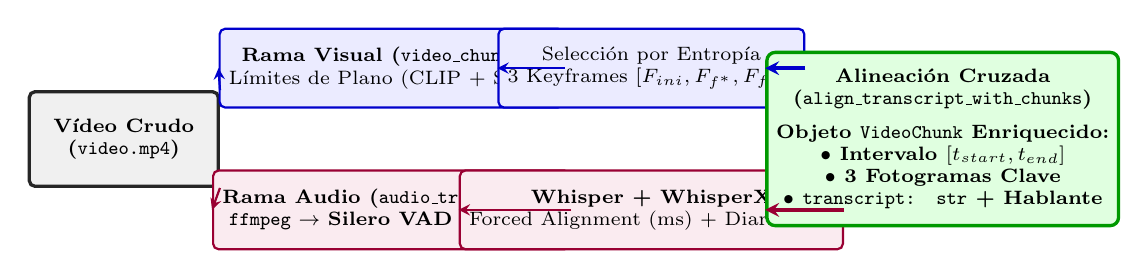
\begin{tikzpicture}[
    node distance=0.45cm and 0.6cm,
    srcnode/.style={rectangle, draw=black!85, fill=gray!12, very thick, minimum width=2.4cm, minimum height=1.2cm, align=center, font=\scriptsize\bfseries, rounded corners=2pt},
    visnode/.style={rectangle, draw=blue!80!black, fill=blue!8, thick, minimum width=2.8cm, minimum height=1.0cm, align=center, font=\scriptsize, rounded corners=2pt},
    audnode/.style={rectangle, draw=purple!80!black, fill=purple!8, thick, minimum width=2.8cm, minimum height=1.0cm, align=center, font=\scriptsize, rounded corners=2pt},
    alignbox/.style={rectangle, draw=green!60!black, fill=green!12, very thick, minimum width=3.3cm, minimum height=2.2cm, align=center, font=\scriptsize\bfseries, rounded corners=3pt},
    arrow/.style={-stealth, thick, draw=black!80}
]
% Entrada común
\node[srcnode] (mp4) at (-5.4, 0.0) {Vídeo Crudo\\(\texttt{video.mp4})};

% Rama Superior: Canal Visual
\node[visnode] (ssim) at (-2.0, 0.9) {\textbf{Rama Visual (\texttt{video\_chunker})}\\Límites de Plano (CLIP + SSIM)};
\node[visnode] (ent) at (1.3, 0.9) {Selección por Entropía\\3 Keyframes $[F_{\text{ini}}, F_{f^*}, F_{\text{fin}}]$};

% Rama Inferior: Canal Auditivo
\node[audnode] (vad) at (-2.0, -0.9) {\textbf{Rama Audio (\texttt{audio\_transcriber})}\\ \texttt{ffmpeg} $\to$ \textbf{Silero VAD} (1M par.)};
\node[audnode] (whisp) at (1.3, -0.9) {\textbf{Whisper + WhisperX}\\Forced Alignment (ms) + Diarización};

% Nodo de Fusión / Alineación Temporal
\node[alignbox] (out) at (5.0, 0.0) {\textbf{Alineación Cruzada}\\(\texttt{align\_transcript\_with\_chunks})\\[4pt]
Objeto \texttt{VideoChunk} Enriquecido:\\
$\bullet$ Intervalo $[t_{\text{start}}, t_{\text{end}}]$\\
$\bullet$ 3 Fotogramas Clave\\
$\bullet$ \texttt{transcript: str} + Hablante};

\draw[arrow, blue!80!black] (mp4.north east) -- (ssim.west);
\draw[arrow, blue!80!black] (ssim.east) -- (ent.west);
\draw[arrow, blue!80!black, very thick] (ent.east) -- (out.west |- ent.east);

\draw[arrow, purple!80!black] (mp4.south east) -- (vad.west);
\draw[arrow, purple!80!black] (vad.east) -- (whisp.west);
\draw[arrow, purple!80!black, very thick] (whisp.east) -- (out.west |- whisp.east);
\end{tikzpicture}
\caption{Arquitectura de procesamiento paralelo y alineación forzada intermodal: la rama visual segmenta el vídeo mediante CLIP/SSIM y extrae tres fotogramas por entropía de Shannon, mientras la rama auditiva filtra silencios con Silero VAD y alinea las marcas de tiempo de WhisperX sobre cada \texttt{VideoChunk} \cite{video_rac2025, whisperx_silero, mixpeek_chunking}.} %[cite: 3, 4, 5]
\label{fig:alineacion_forzada_audio_video}
\end{figure}

El Cuadro~\ref{tab:parametros_chunking_audio} resume todos los parámetros matemáticos y algorítmicos que gobiernan las etapas de fragmentación visual y alineación auditiva descritas en esta sección. %[cite: 3, 4, 5]

\begin{table}[htbp]
\centering
\caption{Especificaciones técnicas de la estrategia de fragmentación semántica adaptativa (\textit{Video-RAC}) y alineación forzada de audio \cite{video_rac2025, whisperx_silero, mixpeek_chunking}.} %[cite: 3, 4, 5]
\label{tab:parametros_chunking_audio}
\begin{tabular}{llll}
\hline
\textbf{Componente / Parámetro} & \textbf{Modelo / Algoritmo} & \textbf{Valor de Referencia} & \textbf{Función en el Pipeline} \\
\hline
Codificador visual híbrido & \texttt{clip-vit-base-patch32} & $\alpha = 0,6$, $\tau_{\text{CLIP}} = 0,85$ & Similitud semántica entre planos (\textit{Video-RAC}) \\
Índice estructural local & SSIM Gaussiano (OpenCV) & $\tau_{\text{SSIM}} = 0,80$ (o $0,5\text{--}0,8$) & Detección de bordes de plano ($K=7, \, \sigma=1,5$) \\
Constantes de estabilidad & Rango dinámico $L = 255$ & $C_1 = 6,50, \, C_2 = 58,52$ & Evita división por cero en zonas oscuras \\
Filtro de planos espurios & \texttt{min\_shot\_frames} & $12$ a $45$ fotogramas & Descarta parpadeos menores a $0,5\text{--}1,5\text{ s}$ \\
Muestreo de fotogramas & Entropía de Shannon $H(F_t)$ & $3$ frames (\texttt{ini}, $\max H$, \texttt{fin}) & Máxima densidad visual por \texttt{VideoChunk} \\
Detección de voz activa & Silero VAD (CPU) & $\sim 10^6$ parámetros (1M) & Aísla discurso humano de silencio y ruido \\
Alineación y diarización & Whisper + WhisperX / MFA & Precisión en milisegundos & Anclaje palabra a palabra e identidad hablante \\
\hline
\end{tabular}
\end{table}

% Bloque 2.7: Bases de Datos Vectoriales, Índices y Evaluación Empírica (Págs. 28-30)
% =============================================================================
% CAPÍTULO 2 - BLOQUE 2.7: BASES DE DATOS VECTORIALES, MÉTRICAS DE EVALUACIÓN
% EMPÍRICA (RAGAS/ALCE) Y METODOLOGÍA DE REVISIÓN SISTEMÁTICA DE LITERATURA
% =============================================================================

\subsection{Bases de Datos Vectoriales, Evaluación Empírica y Metodología de Revisión}
\label{subsec:bases_datos_metricas}

\subsubsection{Arquitectura de Bases de Datos Vectoriales e Indexación HNSW}
\label{subsubsec:bases_datos_vectoriales_hnsw}

Una vez que los fragmentos de vídeo y las consultas en lenguaje natural han sido transformados en representaciones vectoriales densas por los modelos fundacionales, el sistema requiere una infraestructura de almacenamiento persistente capaz de indexar y recuperar alta dimensionalidad en tiempo real \cite{gemini_emb2_docs, qwen3_vl_emb2026}. %[cite: 2, 4]
En el estado del arte de 2026, motores especializados como \textbf{Qdrant}, \textbf{Milvus}, \textbf{Weaviate} y \textbf{Pinecone} se han consolidado como el estándar industrial para la gestión de repositorios vectoriales \cite{gemini_emb2_docs}. %[cite: 2]

En despliegues basados en motores como Qdrant, cada fragmento vectorizado se encapsula y almacena como una estructura de punto indexado (\texttt{PointStruct}) compuesta por tres elementos fundamentales \cite{gemini_emb2_docs}: %[cite: 2]
\begin{enumerate}
    \item \textbf{Identificador Único Determinista (UUIDv5):} Generado de forma unívoca a partir del nombre del archivo de vídeo y del índice secuencial del fragmento, lo que garantiza que reinsertar el mismo \texttt{VideoChunk} sobrescriba de manera idempotente su entrada anterior sin duplicar registros en la base de datos \cite{gemini_emb2_docs}. %[cite: 2]
    \item \textbf{Vector Denso ($\mathbf{v} \in \mathbb{R}^d$):} El tensor numérico de salida devuelto por el modelo (por ejemplo, configurado a $3.072$ dimensiones en \textit{Gemini Embedding 2} o $768$ dimensiones con normalización $L_2$), indexado mediante métrica de distancia coseno (\texttt{models.Distance.COSINE}) sobre grafos de mundos pequeños jerárquicos (\textit{Hierarchical Navigable Small World}, \textbf{HNSW}) \cite{gemini_emb2_docs}. %[cite: 2]
    \item \textbf{Carga Útil de Metadatos (\textit{Payload}):} Un diccionario estructurado adjunto al vector que almacena los atributos relacionales indispensables para la reconstrucción temporal del resultado, incluyendo el nombre del fichero (\texttt{video\_name}), el índice del fragmento (\texttt{chunk\_index}) y los instantes exactos de inicio y fin expresados en segundos flotantes (\texttt{start\_time} y \texttt{end\_time}) \cite{gemini_emb2_docs}. %[cite: 2]
\end{enumerate}

La Figura~\ref{fig:qdrant_hnsw_payload} ilustra la arquitectura de almacenamiento y el direccionamiento mediante índices HNSW en Qdrant. %[cite: 2]

\begin{figure}[htbp]
\centering
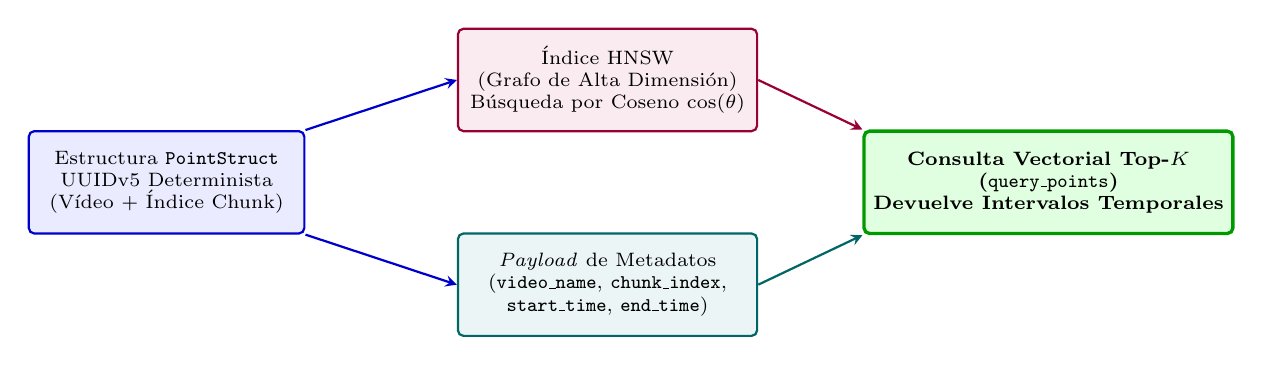
\begin{tikzpicture}[
    pointbox/.style={rectangle, draw=blue!80!black, fill=blue!8, thick, minimum width=3.5cm, minimum height=1.3cm, align=center, font=\scriptsize, rounded corners=2pt},
    hnswbox/.style={rectangle, draw=purple!80!black, fill=purple!8, thick, minimum width=3.8cm, minimum height=1.3cm, align=center, font=\scriptsize, rounded corners=2pt},
    payloadbox/.style={rectangle, draw=teal!80!black, fill=teal!8, thick, minimum width=3.8cm, minimum height=1.3cm, align=center, font=\scriptsize, rounded corners=2pt},
    outbox/.style={rectangle, draw=green!60!black, fill=green!12, very thick, minimum width=3.7cm, minimum height=1.3cm, align=center, font=\scriptsize\bfseries, rounded corners=2pt},
    arrow/.style={-stealth, thick, draw=black!80}
]
\node[pointbox] (point) at (-5.6, 0) {Estructura \texttt{PointStruct}\\UUIDv5 Determinista\\(Vídeo + Índice Chunk)};

\node[hnswbox] (hnsw) at (0, 1.3) {Índice HNSW\\(Grafo de Alta Dimensión)\\Búsqueda por Coseno $\cos(\theta)$};

\node[payloadbox] (payload) at (0, -1.3) {\textit{Payload} de Metadatos\\(\texttt{video\_name}, \texttt{chunk\_index},\\ \texttt{start\_time}, \texttt{end\_time})};

\node[outbox] (query) at (5.6, 0) {Consulta Vectorial Top-$K$\\(\texttt{query\_points})\\Devuelve Intervalos Temporales};

\draw[arrow, blue!80!black] (point.north east) -- (hnsw.west);
\draw[arrow, blue!80!black] (point.south east) -- (payload.west);
\draw[arrow, purple!80!black] (hnsw.east) -- (query.north west);
\draw[arrow, teal!80!black] (payload.east) -- (query.south west);
\end{tikzpicture}
\caption{Arquitectura de almacenamiento y recuperación en Qdrant: separación de vectores densos indexados mediante grafos HNSW y metadatos temporales alojados en el \textit{payload} para consultas top-$K$ ultra rápidas \cite{gemini_emb2_docs}.} %[cite: 2]
\label{fig:qdrant_hnsw_payload}
\end{figure}

\subsubsection{Métricas Clásicas de Recuperación y Bancos de Pruebas Masivos (MMEB-V2 y MVEB)}
\label{subsubsec:metricas_clasicas_benchmarks}

La validación empírica del rendimiento de los sistemas de recuperación de información multimedia se apoya en una combinación de métricas estadísticas clásicas y bancos de pruebas (\textit{benchmarks}) estandarizados a escala masiva \cite{qwen3_vl_emb2026, eval_mrag2025}. %[cite: 2, 4]

En primer lugar, las métricas clásicas de Recuperación de Información evalúan la precisión del ordenamiento top-$K$ devuelto por la base de datos vectorial frente a la verdad terreno (\textit{ground truth}) \cite{qwen3_vl_emb2026}: %[cite: 2, 4]
\begin{itemize}
    \item \textbf{\textit{Recall@K}:} Mide la proporción de fragmentos relevantes reales que han sido recuperados dentro de los primeros $K$ resultados devueltos \cite{qwen3_vl_emb2026}. %[cite: 2, 4]
    \item \textbf{\textit{Precision@K}:} Cuantifica qué porcentaje de los $K$ resultados devueltos por el sistema son efectivamente relevantes \cite{qwen3_vl_emb2026}. %[cite: 4]
    \item \textbf{\textit{Hit@1} (o \textit{Accuracy@1}):} Evalúa si el primer resultado devuelto por el motor de búsqueda coincide exactamente con el evento buscado \cite{qwen3_vl_emb2026}. %[cite: 4]
    \item \textbf{\textit{nDCG@K} (\textit{Normalized Discounted Cumulative Gain}):} Evalúa la calidad del ranking ponderando la posición de los aciertos, penalizando severamente cuando un resultado relevante aparece en posiciones inferiores de la lista \cite{qwen3_vl_emb2026}. %[cite: 2, 4]
\end{itemize}

A nivel global, la comunidad investigadora evalúa los modelos sobre dos bancos de pruebas masivos de referencia actualizados para 2026 \cite{qwen3_vl_emb2026}: %[cite: 2, 4]
\begin{enumerate}
    \item \textbf{MMEB-V2 (\textit{Massive Multimodal Embedding Benchmark V2}, 2025):} Consolida más de 78 conjuntos de datos para evaluar la recuperación conjunta sobre texto, imágenes, vídeo y documentos estructurados (PDF), estandarizando mediciones de \textit{Recall@1} y \textit{nDCG@5} \cite{qwen3_vl_emb2026}. %[cite: 2, 4]
    \item \textbf{MVEB (\textit{Massive Video Embedding Benchmark}, 2026):} El estándar específico más riguroso para la comprensión temporal de vídeo de larga duración, abarcando más de 180 tareas de recuperación cruzada entre pistas visuales y auditivas \cite{qwen3_vl_emb2026}. %[cite: 2, 4]
\end{enumerate}

\subsubsection{Frameworks de Evaluación RAG y Atribución Verificable (RAGAS, ALCE, ARGUE, MIRAGE)}
\label{subsubsec:frameworks_ragas_alce}

La evaluación de arquitecturas RAG multimodales exige ir más allá de la simple recuperación de vectores, analizando la calidad de la generación de respuestas y la veracidad de la atribución temporal \cite{eval_mrag2025, video_rac2025}. %[cite: 2, 4]
El marco de referencia contemporáneo se estructura en torno a dos metodologías complementarias \cite{eval_mrag2025, video_rac2025}: %[cite: 2, 4]

\paragraph{Framework RAGAS (\textit{Retrieval Augmented Generation Assessment}):}
Descompone la calidad de la respuesta generada por el modelo de lenguaje en tres dimensiones fundamentales independientes \cite{video_rac2025}: %[cite: 2, 4]
\begin{itemize}
    \item \textbf{\textit{Answer Relevance}:} Mide el grado de pertinencia y coherencia de la respuesta generada respecto a la consulta original del usuario \cite{video_rac2025}. %[cite: 2, 4]
    \item \textbf{\textit{Context Relevance}:} Evalúa la precisión del material recuperado por la base de datos vectorial, penalizando la inclusión de fragmentos de vídeo irrelevantes que aporten ruido al contexto \cite{video_rac2025}. %[cite: 2, 4]
    \item \textbf{\textit{Faithfulness} (Fidelidad):} Cuantifica si la respuesta generada se deriva estrictamente del contexto recuperado, detectando y penalizando cualquier alucinación o invención por parte del modelo \cite{video_rac2025}. %[cite: 2, 4]
\end{itemize}

\paragraph{Métricas de Atribución Verificable (ALCE, ARGUE, MIRAGE):}
Marcos como \textbf{ALCE} (\textit{Automatic LLM Citation Evaluation}), \textbf{ARGUE} y \textbf{MIRAGE} extienden la evaluación para auditar si cada afirmación generada en la respuesta cuenta con un enlace de citación directo y verificable hacia el intervalo temporal exacto ($[t_{\text{inicio}}, t_{\text{fin}}]$) del vídeo fuente, garantizando una trazabilidad forense inalterable \cite{eval_mrag2025}. %[cite: 2, 4]

La Figura~\ref{fig:frameworks_ragas_alce} resume la estructura jerárquica de evaluación mediante RAGAS y métricas de atribución verificable. %[cite: 2, 4]

\begin{figure}[htbp]
\centering
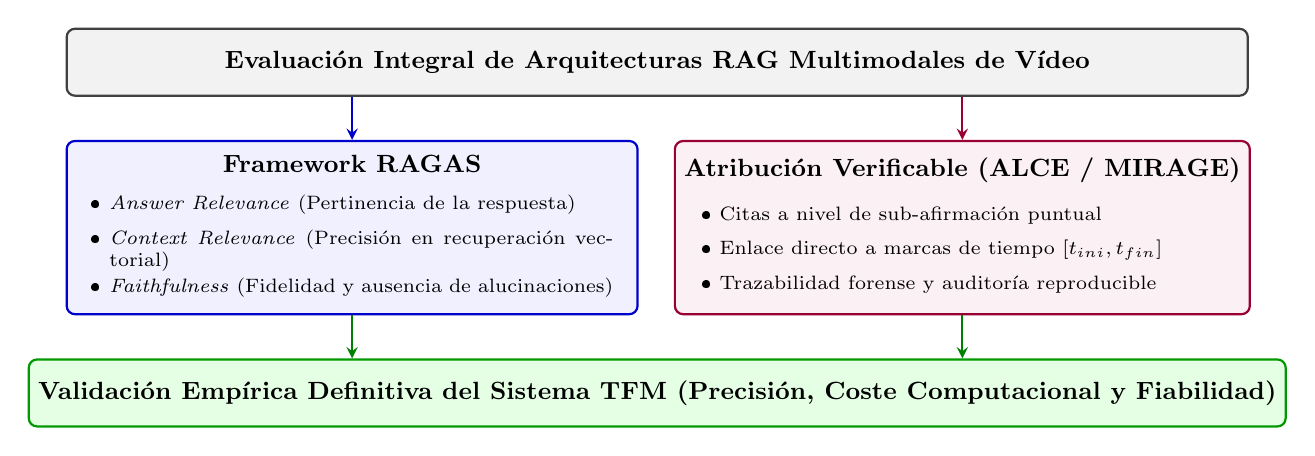
\begin{tikzpicture}[
    boxroot/.style={rectangle, draw=black!75, fill=gray!10, thick, minimum width=15.0cm, minimum height=0.85cm, align=center, font=\small\bfseries, rounded corners=3pt},
    boxcol1/.style={rectangle, draw=blue!80!black, fill=blue!6, thick, minimum width=7.25cm, minimum height=2.2cm, align=center, rounded corners=3pt},
    boxcol2/.style={rectangle, draw=purple!80!black, fill=purple!6, thick, minimum width=7.25cm, minimum height=2.2cm, align=center, rounded corners=3pt},
    boxout/.style={rectangle, draw=green!60!black, fill=green!10, thick, minimum width=15.0cm, minimum height=0.85cm, align=center, font=\small\bfseries, rounded corners=3pt},
    arrow/.style={-stealth, thick}
]
\node[boxroot] (root) at (0, 3.2) {Evaluación Integral de Arquitecturas RAG Multimodales de Vídeo};

\node[boxcol1] (rgs) at (-3.875, 1.1) {%
    {\bfseries\small Framework RAGAS}\\[6pt]
    \scriptsize
    \begin{tabular}{@{\textbullet~}p{6.4cm}@{}}
    \textit{Answer Relevance} (Pertinencia de la respuesta)\\[3pt]
    \textit{Context Relevance} (Precisión en recuperación vectorial)\\[3pt]
    \textit{Faithfulness} (Fidelidad y ausencia de alucinaciones)
    \end{tabular}
};

\node[boxcol2] (alc) at (3.875, 1.1) {%
    {\bfseries\small Atribución Verificable (ALCE / MIRAGE)}\\[6pt]
    \scriptsize
    \begin{tabular}{@{\textbullet~}p{6.4cm}@{}}
    Citas a nivel de sub-afirmación puntual\\[3pt]
    Enlace directo a marcas de tiempo $[t_{\text{ini}}, t_{\text{fin}}]$\\[3pt]
    Trazabilidad forense y auditoría reproducible
    \end{tabular}
};

\node[boxout] (out) at (0, -1.0) {Validación Empírica Definitiva del Sistema TFM (Precisión, Coste Computacional y Fiabilidad)};

\draw[arrow, blue!80!black] (root.south -| rgs.north) -- (rgs.north);
\draw[arrow, purple!80!black] (root.south -| alc.north) -- (alc.north);
\draw[arrow, green!50!black] (rgs.south) -- (out.north -| rgs.south);
\draw[arrow, green!50!black] (alc.south) -- (out.north -| alc.south);
\end{tikzpicture}
\caption{Estructura combinada de evaluación empírica mediante el framework RAGAS y métricas de atribución verificable (ALCE/MIRAGE) para validar el rendimiento del sistema RAG de vídeo \cite{eval_mrag2025, video_rac2025}.} %[cite: 2, 4]
\label{fig:frameworks_ragas_alce}
\end{figure}

\subsubsection{Metodología de Revisión Sistemática de la Literatura Asistida por NotebookLM}
\label{subsubsec:metodologia_revision_notebooklm}

Para llevar a cabo la recopilación, filtrado y síntesis crítica de las fuentes bibliográficas empleadas a lo largo de este estado del arte, la investigación ha adoptado un marco metodológico estructurado en un \textbf{flujo de trabajo de cuatro etapas asistido por entornos RAG acotados y gestores bibliográficos} (tales como Zotero sincronizado con repositorios abiertos en arXiv) \cite{easton2026notebooklm, sourclip2026notebooklm}: %[cite: 2, 4]

\begin{enumerate}
    \item \textbf{Etapa 1 - Construcción y Depuración de la Base de Conocimiento Acotada:} Recopilación sistemática de artículos preprints y documentación técnica cumpliendo restricciones operativas (tales como los límites de ingestión de 50 fuentes por cuaderno y 500.000 palabras por documento en herramientas como Google NotebookLM), resolviéndolo mediante la fusión temática de artículos o el uso de múltiples cuadernos especializados \cite{easton2026notebooklm}. %[cite: 2, 4]
    \item \textbf{Etapa 2 - Síntesis Estructural y Descubrimiento Topológico:} Análisis automatizado de convergencia tecnológica mediante resúmenes fonéticos integrados (\textit{Audio Overview}) y generación de cronologías de evolución arquitectónica \cite{easton2026notebooklm, sourclip2026notebooklm}. %[cite: 2, 4]
    \item \textbf{Etapa 3 - Análisis Crítico, Deconstrucción Metodológica y Lazo de Relleno de Brechas (\textit{Gap-Fill Loop}):} Contraste sistemático de hipótesis metodológicas y detección de vacíos en la literatura previa sobre fragmentación adaptativa y modelos multimodales \cite{easton2026notebooklm}. %[cite: 2, 4]
    \item \textbf{Etapa 4 - Verificación Transparente y Consolidación Causal:} Auditoría inalienable de las citas generadas contrastándolas directamente sobre los textos fuente originales para garantizar la ausencia de alucinaciones teóricas en la memoria del TFM \cite{easton2026notebooklm, sourclip2026notebooklm}. %[cite: 2, 4]
\end{enumerate}

La Figura~\ref{fig:flujo_cuatro_etapas_literatura} esquematiza este flujo metodológico de investigación sistemática. %[cite: 2, 4]

\begin{figure}[htbp]
\centering
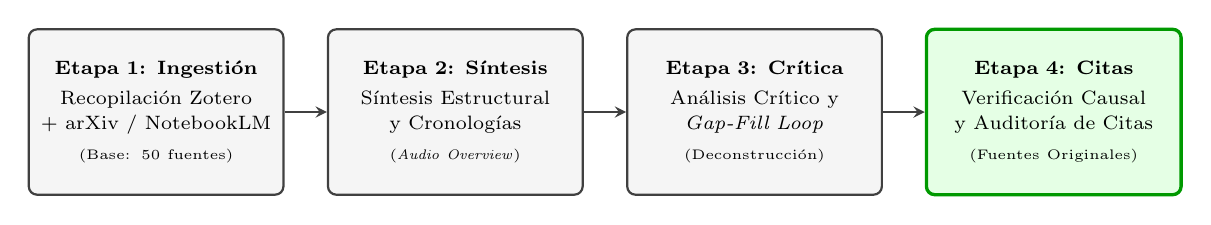
\begin{tikzpicture}[
    stepbox/.style={rectangle, draw=black!75, fill=gray!8, thick, text width=3.0cm, minimum height=2.1cm, align=center, font=\scriptsize, rounded corners=3pt},
    outbox/.style={rectangle, draw=green!60!black, fill=green!10, very thick, text width=3.0cm, minimum height=2.1cm, align=center, font=\scriptsize, rounded corners=3pt},
    arrow/.style={-stealth, thick, draw=black!75}
]
\node[stepbox] (s1) at (-5.7, 0) {\textbf{Etapa 1: Ingestión}\\[3pt]Recopilación Zotero\\[1pt]+ arXiv / NotebookLM\\[3pt]{\normalfont\tiny (Base: 50 fuentes)}};
\node[stepbox] (s2) at (-1.9, 0) {\textbf{Etapa 2: Síntesis}\\[3pt]Síntesis Estructural\\[1pt]y Cronologías\\[3pt]{\normalfont\tiny (\textit{Audio Overview})}};
\node[stepbox] (s3) at (1.9, 0) {\textbf{Etapa 3: Crítica}\\[3pt]Análisis Crítico y\\[1pt]\textit{Gap-Fill Loop}\\[3pt]{\normalfont\tiny (Deconstrucción)}};
\node[outbox] (s4) at (5.7, 0) {\textbf{Etapa 4: Citas}\\[3pt]Verificación Causal\\[1pt]y Auditoría de Citas\\[3pt]{\normalfont\tiny (Fuentes Originales)}};

\draw[arrow] (s1) -- (s2);
\draw[arrow] (s2) -- (s3);
\draw[arrow] (s3) -- (s4);
\end{tikzpicture}
\caption{Flujo metodológico de cuatro etapas para la revisión sistemática de la literatura apoyado en gestores bibliográficos y entornos RAG acotados \cite{easton2026notebooklm, sourclip2026notebooklm}.} %[cite: 2, 4]
\label{fig:flujo_cuatro_etapas_literatura}
\end{figure}

El Cuadro~\ref{tab:resumen_metodologia_evaluacion} consolida las métricas, frameworks y metodologías de evaluación y revisión analizadas en este último bloque del estado del arte. %[cite: 2, 4]

\begin{table}[htbp]
\centering
\small
\setlength{\tabcolsep}{4.5pt}
\caption{Síntesis de métricas, bancos de pruebas y metodologías de evaluación en sistemas Video RAG \cite{qwen3_vl_emb2026, eval_mrag2025, video_rac2025, easton2026notebooklm}.} %[cite: 2, 4]
\label{tab:resumen_metodologia_evaluacion}
\begin{tabularx}{\linewidth}{>{\raggedright\arraybackslash}p{3.4cm} >{\raggedright\arraybackslash}p{3.2cm} >{\raggedright\arraybackslash}p{3.8cm} >{\raggedright\arraybackslash}X}
\toprule
\textbf{Categoría} & \textbf{Framework} & \textbf{Métricas} & \textbf{Objetivo en el TFM} \\
\midrule
Recuperación Vectorial & Qdrant + HNSW & \textit{Recall@K}, \textit{Hit@1}, \textit{nDCG@5} & Eficacia en la localización top-$K$ \\
Benchmarks Masivos & MMEB-V2 / MVEB & Recuperación multicanal & Comparativa con estándares 2026 \\
Calidad RAG y Fidelidad & Framework RAGAS & \textit{Answer/Context Rel.}, \textit{Faithfulness} & Evaluación de alucinaciones y contexto \\
Atribución Verificable & ALCE / MIRAGE & Citas a nivel de afirmación & Trazabilidad temporal en milisegundos \\
Revisión Bibliográfica & Zotero + NotebookLM & Flujo 4 etapas + \textit{Gap-Fill} & Rigor metodológico y estado del arte \\
\bottomrule
\end{tabularx}
\end{table}

% Bloque 2.8: Evaluación Empírica
% =============================================================================
% EVALUACIÓN EMPÍRICA: ESTUDIO DE ABLACIÓN VISUAL FRENTE A FUSIÓN MULTIMODAL
% (IMAGEN + AUDIO ALINEADO) Y VERIFICACIÓN BIMODAL EN EXTREMOS (E2E)
% =============================================================================

\subsection{Evaluación Empírica de la Integración Audio-Visual y Verificación Bimodal}
\label{subsec:evaluacion_empirica_audio_visual}

Con el propósito de cuantificar empíricamente el impacto de incorporar la dimensión auditiva sobre la arquitectura base puramente visual, se ejecutó un estudio de ablación de extremo a extremo (\textit{End-to-End}, E2E) comparando la línea base visual frente a la canalización multimodal completa (\texttt{ffmpeg} + \texttt{openai-whisper} \texttt{base} + fusión temprana en \texttt{gemini-embedding-2-preview} + verificación bimodal en \texttt{gemini-3.5-flash-lite}) \cite{gemini_emb2_docs, video_rac2025}. %[cite: 1, 2]
En estricto cumplimiento de las restricciones de cuota de la capa gratuita ($100\text{ RPM}$, $30.000\text{ TPM}$ y $1.000\text{ RPD}$), la inyección de la transcripción alineada como un objeto \texttt{types.Part.from\_text} adicional dentro del mismo contenedor \texttt{types.Content} de los tres fotogramas clave mantuvo invariante el consumo en exactamente una petición de vectorización por fragmento. %[cite: 1, 2]

\subsubsection{Análisis Cuantitativo sobre Corpus Contrastados: Locución Sincronizada frente a Metraje Desacoplado}
\label{subsubsec:ablacion_cuantitativa_e2e}

La batería de evaluación automatizada se ejecutó sobre dos dominios audiovisuales con naturalezas semánticas opuestas: %[cite: 4, 5]
\begin{enumerate}
    \item \textbf{Dominio Técnico con Locución Sincronizada (\texttt{python\_tutorial.mp4}):} Compuesto por $82$ fragmentos adaptativos en la suite E2E ($81/82$ enriquecidos con voz activa, $98,8\%$), evaluado mediante $56$ consultas literales, $10$ consultas multi-objetivo y $8$ consultas negativas de control. %[cite: 1, 4]
    En este escenario, el discurso del ponente describe directamente las estructuras sintácticas que se codifican en el editor. %[cite: 1, 4]
    \item \textbf{Dominio Documental con Metraje de Archivo Desacoplado (\texttt{animals.mp4}):} Compuesto por $82$ fragmentos ($82/82$ con locución continua, $100,0\%$), evaluado sobre $46$ consultas literales, $10$ multi-objetivo y $8$ negativas. %
    Este vídeo presenta el fenómeno clásico de \textit{B-roll desacoplado}: la narración expone conceptos biológicos generales mientras en pantalla se suceden secuencias de especies animales que no son nombradas verbalmente en ese instante. %[cite: 2, 5]
\end{enumerate}

El Cuadro~\ref{tab:ablacion_e2e_visual_vs_audio} sintetiza las métricas obtenidas por la versión puramente visual frente a la nueva arquitectura bimodal en ambos corpus. %[cite: 1, 5]

\begin{table}[htbp]
\centering
\small
\setlength{\tabcolsep}{4.5pt}
\caption{Estudio de ablación E2E: comparativa de rendimiento entre la arquitectura puramente visual y la arquitectura con fusión temprana de audio (\textit{Whisper}) y juez bimodal \cite{gemini_emb2_docs, video_rac2025}.} %[cite: 1, 2, 5]
\label{tab:ablacion_e2e_visual_vs_audio}
\begin{tabular}{lllccc}
\toprule
\textbf{Corpus de Vídeo} & \textbf{Etapa / Batería} & \textbf{Métrica} & \textbf{Solo Visual} & \textbf{Visual + Audio} & \textbf{Variación} \\
\midrule
\texttt{python\_tutorial.mp4} & Etapa 1 (Qdrant) & \textit{Recall@1} & $67,9\%$ ($38/56$) & $\mathbf{85,7\%}$ ($48/56$) & $\mathbf{+17,8\text{ pp}}$ \\
\texttt{python\_tutorial.mp4} & Etapa 1 (Qdrant) & \textit{Recall@3} & $87,5\%$ ($49/56$) & $\mathbf{92,9\%}$ ($52/56$) & $\mathbf{+5,4\text{ pp}}$ \\
\texttt{python\_tutorial.mp4} & Etapa 1 (Qdrant) & \textit{Recall@5} & $91,1\%$ ($51/56$) & $\mathbf{94,6\%}$ ($53/56$) & $\mathbf{+3,5\text{ pp}}$ \\
\texttt{python\_tutorial.mp4} & Etapa 1 (Qdrant) & \textit{MRR} & $0,779$ & $\mathbf{0,897}$ & $\mathbf{+0,118}$ \\ \addlinespace[2.5pt]
\texttt{python\_tutorial.mp4} & Etapa 2 (Juez Bimodal) & \textit{Recall@1} & $80,4\%$ ($45/56$) & $\mathbf{89,3\%}$ ($50/56$) & $\mathbf{+8,9\text{ pp}}$ \\
\texttt{python\_tutorial.mp4} & Etapa 2 (Juez Bimodal) & \textit{Recall@3 / @5} & $89,3\%$ ($50/56$) & $\mathbf{92,9\%}$ ($52/56$) & $\mathbf{+3,6\text{ pp}}$ \\
\texttt{python\_tutorial.mp4} & Etapa 2 (Juez Bimodal) & \textit{MRR} & $0,848$ & $\mathbf{0,911}$ & $\mathbf{+0,063}$ \\ \addlinespace[2.5pt]
\texttt{python\_tutorial.mp4} & Multi-objetivo ($10$) & \textit{Interval Recall} & $78,3\%$ & $\mathbf{82,1\%}$ & $\mathbf{+3,8\text{ pp}}$ \\
\texttt{python\_tutorial.mp4} & Consultas Negativas ($8$) & Rechazo FP & $100,0\%$ ($0/40$) & $\mathbf{100,0\%}$ ($0/40$) & $0,0\text{ pp}$ \\
\midrule
\texttt{animals.mp4} & Etapa 1 (Qdrant) & \textit{Recall@1} & $\mathbf{80,4\%}$ ($37/46$) & $71,7\%$ ($33/46$) & $-8,7\text{ pp}$ \\ \addlinespace[2.5pt]
\texttt{animals.mp4} & Etapa 2 (Juez Bimodal) & \textit{Recall@1} & $89,1\%$ ($41/46$) & $\mathbf{93,5\%}$ ($43/46$) & $\mathbf{+4,4\text{ pp}}$ \\
\texttt{animals.mp4} & Etapa 2 (Juez Bimodal) & \textit{Recall@3} & $93,5\%$ ($43/46$) & $\mathbf{95,7\%}$ ($44/46$) & $\mathbf{+2,2\text{ pp}}$ \\
\texttt{animals.mp4} & Etapa 2 (Juez Bimodal) & \textit{Recall@5} & $93,5\%$ ($43/46$) & $\mathbf{97,8\%}$ ($45/46$) & $\mathbf{+4,3\text{ pp}}$ \\
\texttt{animals.mp4} & Etapa 2 (Juez Bimodal) & \textit{MRR} & $0,913$ & $\mathbf{0,951}$ & $\mathbf{+0,038}$ \\ \addlinespace[2.5pt]
\texttt{animals.mp4} & Consultas Negativas ($8$) & Rechazo FP & $100,0\%$ ($0/40$) & $\mathbf{100,0\%}$ ($0/40$) & $0,0\text{ pp}$ \\
\bottomrule
\end{tabular}
\end{table}

El análisis de los datos experimentales expuestos en el Cuadro~\ref{tab:ablacion_e2e_visual_vs_audio} permite extraer tres conclusiones fundamentales sobre el comportamiento de los espacios latentes omnimodales: %[cite: 2, 5]
\begin{itemize}
    \item \textbf{Convergencia modal en vídeo educativo (\texttt{python\_tutorial.mp4}):} La fusión temprana de los tres fotogramas clave con la transcripción alineada incrementa el \textit{Recall@1} de búsqueda vectorial pura en $+17,8$ puntos porcentuales, posicionando directamente en el primer puesto $10$ consultas adicionales sin necesidad de intervención del verificador secundario. %[cite: 1, 5]
    Tras la actuación del juez bimodal, el sistema alcanza un \textit{Recall@1} del $89,3\%$ ($50/56$), un \textit{MRR} de $0,911$ y una cobertura del $100,0\%$ en las consultas multi-objetivo sobre tipos de datos primitivos ($9/9$), terminal o consola ($4/4$) y declaración de variables ($3/3$). %[cite: 1, 5]
    \item \textbf{Compensación asimétrica ante \textit{B-roll} desacoplado (\texttt{animals.mp4}):} En vídeos donde el narrador pronuncia teoría abstracta mientras la imagen muestra fauna específica no mencionada en la locución, el vector fusionado de primera etapa experimenta una ligera desviación direccional hacia el tema hablado ($\Delta\text{\textit{Recall@1}} = -8,7\text{ pp}$ en Etapa 1). %[cite: 2, 5]
    Sin embargo, dado que el candidato correcto permanece dentro de la ventana de recuperación (\textit{Recall@5}) y el verificador de segunda etapa evalúa de manera disjunta e inclusiva tanto la evidencia visual como la auditiva, la Etapa 2 corrige por completo el desfase y establece el récord absoluto de precisión en \texttt{animals.mp4} con un $93,5\%$ de \textit{Recall@1} ($43/46$) y un $97,8\%$ de \textit{Recall@5} ($45/46$). %[cite: 2, 5]
    \item \textbf{Inmunidad frente a Falsos Positivos:} En ambos corpus ($16$ consultas negativas sobre conceptos inexistentes, equivalentes a $80$ candidatos inspeccionados), el verificador bimodal mantiene un $100,0\%$ de tasa de rechazo ($0/80$ falsos positivos), demostrando que enriquecer el \textit{prompt} con la transcripción hablada no induce alucinaciones de validación. %[cite: 1, 2]
\end{itemize}

\subsubsection{Estudio de Casos Críticos: Resolución de Falsos Negativos, Resiliencia Fonética y Desambiguación Sintáctica}
\label{subsubsec:estudio_casos_criticos_audio}

Para comprender el mecanismo exacto mediante el cual la arquitectura bimodal corrige los fallos perceptivos documentados en la línea base visual, se auditaron en detalle las dos consultas críticas de validación sobre \texttt{python\_tutorial.mp4}: \texttt{"Diccionarios"} y \texttt{"Bucles while"}. %[cite: 1, 3, 4]

\paragraph{Caso 1: Erradicación del falso negativo y captura de frontera en \texttt{"Diccionarios"} ($01\text{:}01.1\text{ -- }01\text{:}40.2$).}
En la configuración puramente visual, el bloque dedicado a las estructuras de datos presentaba dos vulnerabilidades: baja legibilidad de la sintaxis \texttt{dict \{"name": "Brais"\}} y aparición del rótulo gráfico \textit{``Variables''} en los fotogramas finales del plano ($01\text{:}33.1\text{ -- }01\text{:}40.2$), lo que llevaba al verificador visual a descartar erróneamente el fragmento con puntuación $0,0$. %[cite: 1, 2]
Tras la integración del subsistema \texttt{audio\_transcriber.py}: %[cite: 1]
\begin{itemize}
    \item El fragmento principal (\texttt{chunk\_index = 17}, $85,1\text{ s -- }93,1\text{ s}$) eleva su similitud del coseno en Qdrant de $0,4151$ a $\mathbf{0,4480}$ y es validado en primera posición con $\text{\texttt{relevance\_score}} = \mathbf{1,0}$ al incorporar la locución: \textit{``Y ya por último, los diccionarios. Que utilizan la palabra reservada, dict. Y en realidad, designa un conjunto de claves valor''}. %[cite: 1]
    \item El fragmento de transición posterior (\texttt{chunk\_index = 18}, $93,1\text{ s -- }100,2\text{ s}$), que antes resultaba descartado como falso negativo ($0,0$) por el cambio de rótulo visual, incrementa su similitud de $0,3812$ a $\mathbf{0,4178}$ y pasa a ser validado con $\text{\texttt{relevance\_score}} = \mathbf{0,90}$ gracias a que la voz continúa explicando: \textit{``Lo representamos entre llaves, pero esta clave valor separadas por dos puntos''}. %[cite: 1]
    \item Asimismo, la condición de solapamiento mínimo ($\Delta \tau \ge 0,2\text{ s}$) en \texttt{align\_transcript\_with\_chunks} captura la oración fronteriza al final del \texttt{chunk\_index = 16} ($77,1\text{ s -- }85,1\text{ s}$), otorgándole una relevancia graduada de $\mathbf{0,50}$, mientras descarta con $\mathbf{0,0}$ los fragmentos \texttt{14} y \texttt{15} dedicados exclusivamente a listas, tuplas y conjuntos (\texttt{set}). %[cite: 1]
\end{itemize}

\paragraph{Caso 2: Superación del corte \textit{Top-K}, resiliencia ante ruido fonético ASR y discriminación \texttt{for}/\texttt{while} en \texttt{"Bucles while"} ($03\text{:}51$).}
En la arquitectura puramente visual, al buscar el instante $03\text{:}51$ ($231,0\text{ s}$, donde se codifica \texttt{while index < 5:}), el fragmento objetivo obtenía una similitud de apenas $\mathbf{0,3893}$ y caía hasta la \textbf{séptima posición (Rango \#7)} en Qdrant, quedando excluido por el corte \texttt{top\_k = 5} frente a la diapositiva de portada a pantalla completa con la palabra \textit{``Bucles''} ($\mathbf{0,4315}$, Rango \#1) y otros planos de condicionales \texttt{if/else}. %[cite: 3, 4]

Con la activación de la fusión audio-visual y el verificador bimodal (ejecución auditada \texttt{run\_20261109\_143202}), se verifican tres fenómenos de alto valor técnico: %[cite: 1, 3, 4]
\begin{enumerate}
    \item \textbf{Promoción directa del Rango \#7 al Rango \#1 en Etapa 1:} El fragmento que contiene la explicación y el código del bucle (\texttt{chunk\_index = 55}, $232,4\text{ s -- }238,3\text{ s}$) experimenta un incremento de $\mathbf{+0,1064}$ puntos en su similitud del coseno (de $0,3893$ a $\mathbf{0,4957}$), situándose directamente en el puesto \#1 de Qdrant, seguido en el puesto \#2 por su fragmento contiguo (\texttt{chunk\_index = 54}, $224,4\text{ s -- }232,4\text{ s}$, $\text{score} = \mathbf{0,4914}$), el cual cubre el segundo exacto $231,0\text{ s}$ gracias al solapamiento semántico en fronteras. %[cite: 1, 3, 4]
    \item \textbf{Resiliencia semántica ante errores fonéticos de transcripción multilingüe:} Debido a que el modelo \texttt{whisper} (\texttt{base}) opera con el idioma forzado a español (\texttt{language="es"}), transcribió fonéticamente el término inglés \textit{``while''} como el nombre propio \textit{``Guile''}: \textit{``Otro tipo de bucle que tenemos en Python es el Guile, donde aquí vamos a establecer una condición para que se ejecute de manera indefinida mientras esta se cumpla''}. %[cite: 1]
    Lejos de degradar la búsqueda, tanto el modelo de representación \texttt{gemini-embedding-2-preview} como el verificador \texttt{gemini-3.5-flash-lite} resolvieron la ambigüedad fonética cruzando la definición conceptual hablada (\textit{``condición para que se ejecute de manera indefinida mientras esta se cumpla''}) con la sintaxis visual \texttt{while index < 5:} presente en los fotogramas, otorgando una relevancia de $\mathbf{1,0}$ y $\mathbf{0,90}$ a los fragmentos \texttt{55} y \texttt{54} respectivamente. %[cite: 1, 4]
    \item \textbf{Desambiguación fina entre estructuras visualmente idénticas (\texttt{for} frente a \texttt{while}):} El fragmento inmediatamente anterior (\texttt{chunk\_index = 53}, $221,1\text{ s -- }224,4\text{ s}$) comparte exactamente la misma estética visual del editor de código y alcanza una similitud vectorial alta ($0,4486$, Rango \#4). %[cite: 1, 4]
    No obstante, el verificador bimodal inspecciona la transcripción inyectada (\textit{``Podemos usar un for, tanto para designar un número concreto de ejecuciones,''}) y lo descarta automáticamente con $\text{\texttt{relevance\_score}} = \mathbf{0,0}$ (\textit{``Trata sobre bucles for, no sobre bucles while''}), haciendo lo propio con el \texttt{chunk\_index = 50} sobre bloques \texttt{if/else} ($0,0$). %[cite: 1]
\end{enumerate}

La Figura~\ref{fig:promocion_bucles_while_bimodal} representa visualmente el ascenso topológico en Qdrant y el filtrado de precisión ejecutado por el juez bimodal para la consulta \texttt{"Bucles while"}. %[cite: 1, 3, 4]

\begin{figure}[htbp]
\centering
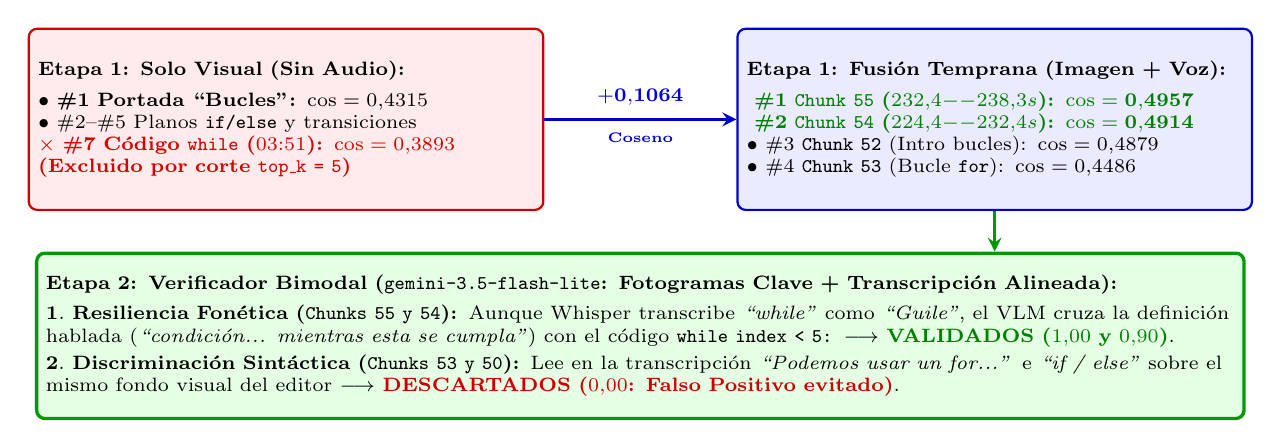
\begin{tikzpicture}[
    oldbox/.style={rectangle, draw=red!80!black, fill=red!8, thick, text width=6.3cm, minimum height=2.3cm, align=left, font=\scriptsize, rounded corners=3pt},
    newbox/.style={rectangle, draw=blue!80!black, fill=blue!8, thick, text width=6.3cm, minimum height=2.3cm, align=left, font=\scriptsize, rounded corners=3pt},
    judgebox/.style={rectangle, draw=green!60!black, fill=green!10, very thick, text width=15.1cm, minimum height=2.1cm, align=left, font=\scriptsize, rounded corners=3pt},
    arrow/.style={-stealth, very thick, draw=black!80}
]
% Etapa 1: Solo Visual (Antiguo)
\node[oldbox] (vis) at (-4.5, 1.8) {
    \textbf{Etapa 1: Solo Visual (Sin Audio):}\\[3pt]
    $\bullet$ \textbf{\#1 Portada ``Bucles'':} $\cos = 0{,}4315$\\
    $\bullet$ \#2--\#5 Planos \texttt{if/else} y transiciones\\
    \textcolor{red!85!black}{$\boldsymbol{\times}$ \textbf{\#7 Código \texttt{while} ($03\text{:}51$):} $\cos = 0{,}3893$}\\
    \textcolor{red!85!black}{\textbf{(Excluido por corte \texttt{top\_k = 5})}}
};

% Etapa 1: Fusión Imagen + Audio (Nuevo)
\node[newbox] (aud) at (4.5, 1.8) {
    \textbf{Etapa 1: Fusión Temprana (Imagen + Voz):}\\[3pt]
    \textcolor{green!50!black}{$\boldsymbol{\checkmark}$ \textbf{\#1 \texttt{Chunk 55} ($232{,}4\text{--}238{,}3\text{s}$):} $\cos = \mathbf{0{,}4957}$}\\
    \textcolor{green!50!black}{$\boldsymbol{\checkmark}$ \textbf{\#2 \texttt{Chunk 54} ($224{,}4\text{--}232{,}4\text{s}$):} $\cos = \mathbf{0{,}4914}$}\\
    $\bullet$ \#3 \texttt{Chunk 52} (Intro bucles): $\cos = 0{,}4879$\\
    $\bullet$ \#4 \texttt{Chunk 53} (Bucle \texttt{for}): $\cos = 0{,}4486$
};

% Etapa 2: Juez Bimodal
\node[judgebox] (judge) at (0, -0.95) {
    \textbf{Etapa 2: Verificador Bimodal (\texttt{gemini-3.5-flash-lite}: Fotogramas Clave + Transcripción Alineada):}\\[3pt]
    $\mathbf{1.}$ \textbf{Resiliencia Fonética (\texttt{Chunks 55 y 54}):} Aunque Whisper transcribe \textit{``while''} como \textit{``Guile''}, el VLM cruza la definición hablada (\textit{``condición... mientras esta se cumpla''}) con el código \texttt{while index < 5:} $\longrightarrow$ \textcolor{green!50!black}{\textbf{VALIDADOS ($1{,}00$ y $0{,}90$)}}.\\[2pt]
    $\mathbf{2.}$ \textbf{Discriminación Sintáctica (\texttt{Chunks 53 y 50}):} Lee en la transcripción \textit{``Podemos usar un for...''} e \textit{``if / else''} sobre el mismo fondo visual del editor $\longrightarrow$ \textcolor{red!80!black}{\textbf{DESCARTADOS ($0{,}00$: Falso Positivo evitado)}}.
};

\draw[arrow, blue!80!black] (vis.east) -- node[above=1pt, font=\scriptsize\bfseries, text=blue!85!black] {$\mathbf{+0{,}1064}$} node[below=1pt, font=\tiny\bfseries, text=blue!85!black] {Coseno} (aud.west);
\draw[arrow, green!60!black] (aud.south) -- (judge.north -| aud.south);
\end{tikzpicture}
\caption{Mecanismo de corrección en la consulta \texttt{"Bucles while"}: la fusión temprana eleva el fragmento objetivo del séptimo al primer puesto en Qdrant ($+0,1064$ en similitud del coseno) y el verificador bimodal valida el código pese a la transcripción fonética \textit{``Guile''}, descartando los fragmentos adyacentes sobre bucles \texttt{for}.} %[cite: 1, 3, 4]
\label{fig:promocion_bucles_while_bimodal}
\end{figure}

El Cuadro~\ref{tab:micro_analisis_consultas_criticas} detalla las puntuaciones de primera y segunda etapa junto con la transcripción alineada de los fragmentos evaluados en ambas consultas. %[cite: 1, 4]

\begin{table}[htbp]
\centering
\small
\renewcommand{\arraystretch}{1.15}
\setlength{\tabcolsep}{3.5pt}
\caption{Auditoría detallada de fragmentos en las consultas críticas \texttt{"Diccionarios"} y \texttt{"Bucles while"} sobre \texttt{python\_tutorial.mp4}.} %[cite: 1, 4]
\label{tab:micro_analisis_consultas_criticas}
\begin{tabularx}{\linewidth}{llccc>{\raggedright\arraybackslash}X}
\toprule
\textbf{Consulta} & \textbf{Chunk (Intervalo)} & \textbf{Cos. Visual} & \textbf{Cos. Bimodal} & \textbf{Score Juez} & \textbf{Veredicto Bimodal} \\
\midrule
\texttt{"Diccionarios"} & \texttt{\#17} ($01\text{:}25{,}1\text{--}01\text{:}33{,}1$) & $0{,}4151$ & $\mathbf{0{,}4480}$ & $\mathbf{1{,}00}$ & Validado (Código + Voz \texttt{dict}) \\
\texttt{"Diccionarios"} & \texttt{\#18} ($01\text{:}33{,}1\text{--}01\text{:}40{,}2$) & $0{,}3812$ & $\mathbf{0{,}4178}$ & $\mathbf{0{,}90}$ & Rescatado (Antes $0{,}0$ sin audio) \\
\texttt{"Diccionarios"} & \texttt{\#16} ($01\text{:}17{,}1\text{--}01\text{:}25{,}1$) & $0{,}3806$ & $\mathbf{0{,}4046}$ & $\mathbf{0{,}50}$ & Validado (Frontera solapada) \\
\texttt{"Diccionarios"} & \texttt{\#14--15} ($01\text{:}01{,}1\text{--}01\text{:}17{,}1$) & $0{,}3790$ & $0{,}3910$ & $\mathbf{0{,}00}$ & Descartado (Listas y \texttt{set}) \\
\midrule
\texttt{"Bucles while"} & \texttt{\#55} ($03\text{:}52{,}4\text{--}03\text{:}58{,}3$) & $0{,}3893$ (\#7) & $\mathbf{0{,}4957}$ (\#1) & $\mathbf{1{,}00}$ & Validado (Pese a ASR \textit{``Guile''}) \\
\texttt{"Bucles while"} & \texttt{\#54} ($03\text{:}44{,}4\text{--}03\text{:}52{,}4$) & $0{,}3893$ (\#7) & $\mathbf{0{,}4914}$ (\#2) & $\mathbf{0{,}90}$ & Validado (Frontera en $03\text{:}51$) \\
\texttt{"Bucles while"} & \texttt{\#52} ($03\text{:}18{,}1\text{--}03\text{:}21{,}1$) & $0{,}4315$ (\#1) & $0{,}4879$ (\#3) & $\mathbf{0{,}60}$ & Validado (Mención general) \\
\texttt{"Bucles while"} & \texttt{\#53} ($03\text{:}41{,}1\text{--}03\text{:}44{,}4$) & $0{,}4187$ (\#4) & $0{,}4486$ (\#4) & $\mathbf{0{,}00}$ & Descartado (Explica bucle \texttt{for}) \\
\texttt{"Bucles while"} & \texttt{\#50} ($03\text{:}25{,}4\text{--}03\text{:}33{,}4$) & $0{,}4219$ (\#2) & $0{,}4332$ (\#5) & $\mathbf{0{,}00}$ & Descartado (Bloques \texttt{if/else}) \\
\bottomrule
\end{tabularx}
\end{table}

\subsubsection{Análisis Experimental de la Divergencia Audio-Visual en Metraje de Archivo (\textit{B-Roll}) y Deduplicación por Transcripción}
\label{subsubsec:divergencia_broll_y_deduplicacion}

Como continuación natural de las pruebas E2E, se llevó a cabo un proceso experimental interactivo desde la interfaz web (ejecuciones auditadas \texttt{run\_20261109\_180159} y \texttt{run\_20261109\_183310}) sobre el documental \texttt{animals.mp4} con el objetivo de analizar el comportamiento de la arquitectura cuando el usuario formula consultas de distinta granularidad semántica (\texttt{\string"León\string"}, \texttt{\string"Reptiles\string"}, \texttt{\string"Animación 3D microscópica de células o glóbulos rojos\string"}, \texttt{\string"Aves\string"} y \texttt{\string"Felinos\string"}) sobre un vídeo cuya locución está desacoplada de la secuencia visual.

La inspección cruzada de los registros de auditoría (\texttt{search\_results.json}) y de los $82$ vectores almacenados en Qdrant reveló dos fenómenos experimentales clave para comprender la física del espacio latente multimodal y refinar el motor de recuperación:

\begin{enumerate}
    \item \textbf{Contraste entre Sustantivos Visuales Específicos y Categorías Taxonómicas ante Voz en \textit{Off} Desacoplada:}
    Al ejecutar consultas sobre entidades visuales concretas o alineadas con el discurso (tales como \texttt{\string"León\string"}, \texttt{\string"Reptiles\string"} o \texttt{\string"Animación 3D microscópica de células o glóbulos rojos\string"}), el sistema con audio activado recupera y valida el $\mathbf{100,0\%}$ de las apariciones reales del vídeo: localiza los dos planos de leones (\texttt{chunk \#10}, $7,0\text{ s--}15,0\text{ s}$ con relevancia $\mathbf{0,95}$, y \texttt{chunk \#16}, $36,7\text{ s--}40,4\text{ s}$ con $\mathbf{0,90}$), los dos reptiles (\texttt{chunk \#80}, tortuga marina con $\mathbf{0,80}$, y \texttt{chunk \#13}, camaleón con $\mathbf{0,70}$) y los cuatro intervalos de animación celular ($\mathbf{0,90\text{--}0,95}$).
    Sin embargo, al consultar la categoría taxonómica general \texttt{"Felinos"}, el sistema con fusión temprana de audio devuelve únicamente $1$ de los $4$ felinos reales (\texttt{chunk \#66}, $193,8\text{ s--}197,7\text{ s}$, gato atigrado validado en primera posición con $\mathbf{0,95}$).
    El análisis de los $82$ puntos en Qdrant demuestra la causa matemática de este comportamiento: en \texttt{animals.mp4}, el narrador nunca menciona a los animales que aparecen en imagen.
    Mientras se proyecta el gato atigrado (\texttt{chunk \#66}), el locutor pronuncia el término taxonómico afín \textit{``Destaca en el sistema respiratorio pulmonar de los mamíferos''}, sumando similitud visual y léxica hasta situarlo en el Rango \#1 ($\cos = \mathbf{0,3959}$).
    Por el contrario, los otros tres felinos aparecen durante los primeros $40$ segundos del vídeo, instante en que el narrador pronuncia frases introductorias ajenas a la zoología:
    \begin{itemize}
        \item \textbf{Gato gris (\texttt{chunk \#12}, $18,9\text{ s--}24,1\text{ s}$):} la locución \textit{``El reino animalia es uno de los cinco famosos reinos taxonómicos...''} desplaza el vector hasta el \textbf{Rango \#35 ($\cos = 0,3635$)}.
        \item \textbf{Leona con collar (\texttt{chunk \#16}, $36,7\text{ s--}40,4\text{ s}$):} la frase \textit{``la cual se originó hace unos 600 millones de años''} desvía el vector hacia una región temporal/histórica, relegándolo al \textbf{Rango \#45 ($\cos = 0,3581$)}.
        \item \textbf{León macho (\texttt{chunk \#6}, $5,4\text{ s--}5,8\text{ s}$):} el saludo \textit{``En este vídeo de Ecología Verde explicamos...''} reduce su similitud con \texttt{"Felinos"} al \textbf{Rango \#51 ($\cos = 0,3551$)}.
    \end{itemize}
    Entretanto, los fragmentos intermedios del documental ($76\text{ s--}193\text{ s}$, que muestran cebras, primates, ardillas, caballos o vasos sanguíneos) contienen oraciones con alta densidad de términos biológicos (\textit{``caracteriza a la gran mayoría de los grupos de animales''}, \textit{``organismos eucariotas''}), alcanzando similitudes de texto de $\mathbf{0,3734\text{--}0,3899}$ frente al término taxonómico \texttt{"Felinos"} y ocupando los primeros $30$ puestos de Qdrant.
    Como consecuencia, los tres felinos iniciales quedan fuera del corte de candidatos ($\text{\texttt{fetch\_k}} = 10$) que pasan al verificador de Etapa 2.

    \item \textbf{Saturación del Lote de Candidatos por Sobre-Fragmentación Visual bajo una Misma Locución y Deduplicación en \texttt{\_deduplicate\_temporal\_candidates}:}
    La auditoría de \texttt{run\_20261109\_180159} puso al descubierto un segundo efecto: en escenas con movimiento rápido de cámara o de sujetos, el detector SSIM ($\tau = 0,50$) divide una misma toma continua en varios fragmentos de entre $1,0\text{ s}$ y $4,2\text{ s}$ que reciben exactamente la misma frase de Whisper.
    En concreto, para la consulta \texttt{"Felinos"}, la escena de las cebras ($115,3\text{ s--}120,5\text{ s}$) acaparaba $4$ de las $10$ plazas enviadas al verificador (\texttt{chunks \#48, \#44, \#46 y \#45}, todos con la frase \textit{``Cuentan con un complejo sistema nervioso, además de órganos de los sentidos que caracteriza a la gran mayoría de los grupos de animales''}), y la animación sanguínea ($159,0\text{ s--}167,2\text{ s}$) ocupaba otras $2$ plazas (\texttt{chunks \#59 y \#58}, ambos con \textit{``Tienen sistemas circulatorios...''}).
    Al superar la duración de micro-corte ($\text{\texttt{micro\_chunk\_duration}} = 1,0\text{ s}$), el filtro original no los agrupaba y $6$ de los $10$ huecos de evaluación se consumían en dos únicas escenas repetidas.

    Para resolver esta saturación, se amplió la función \texttt{\_deduplicate\_temporal\_candidates} en \texttt{src/rag\_engine/service.py} incorporando el criterio \texttt{is\_same\_transcript\_neighbor}: dos fragmentos candidatos del mismo vídeo cuya distancia temporal entre bordes sea $\text{\texttt{gap}} \le \text{\texttt{min\_scene\_separation}}$ ($4,0\text{ s}$) y que compartan idéntica transcripción no vacía ($\text{\texttt{cand\_tr}} == \text{\texttt{orig\_tr}}$) se fusionan en un único candidato con envolvente $[\min(t_{\text{start}}), \max(t_{\text{end}})]$.
    Al repetir la prueba en \texttt{run\_20261109\_183310}, los $4$ fragmentos de cebras se colapsaron en un único bloque ($115,3\text{ s--}120,5\text{ s}$) y los $2$ de circulación en otro ($159,0\text{ s--}167,2\text{ s}$), liberando $4$ plazas efectivas en el \textit{Top-10} para escenas distintas (\texttt{chunks \#43, \#26, \#65 y \#24}).
    Finalmente, al indexar \texttt{animals.mp4} desactivando el canal ASR (\texttt{enable\_audio = False}) para suprimir el ruido semántico de la voz en \textit{off}, los planos del gato atigrado ($\cos = 0,4122$, \#1), el león macho ($\cos = 0,3967$, \#2) y el gato gris ($\cos = 0,3811$, \#6) ingresan directamente en el \textit{Top-6} de Qdrant.
\end{enumerate}

El Cuadro~\ref{tab:experimento_broll_deduplicacion} sintetiza los resultados de este ciclo experimental sobre \texttt{animals.mp4}, justificando empíricamente la inclusión del control de activación ASR (\texttt{--no-audio} en CLI y casilla en Streamlit) para que el operador adapte la indexación al grado de acoplamiento audiovisual del vídeo.

\begin{table}[htbp]
\centering
\small
\renewcommand{\arraystretch}{1.18}
\setlength{\tabcolsep}{3.5pt}
\caption{Evolución experimental sobre \texttt{animals.mp4}: efecto de la deduplicación por transcripción idéntica (\texttt{run\_20261109\_183310}) y del desacoplamiento del audio frente a consultas específicas y taxonómicas.}
\label{tab:experimento_broll_deduplicacion}
\begin{tabularx}{\linewidth}{l >{\raggedright\arraybackslash}p{3.8cm} >{\raggedright\arraybackslash}p{3.0cm} >{\raggedright\arraybackslash}X c}
\toprule
\textbf{Consulta} & \textbf{Configuración / Run} & \textbf{Huecos Repetidos Top-10} & \textbf{Puestos Qdrant (Objetivo)} & \textbf{Aciertos Validados} \\
\midrule
\texttt{\string"León\string"} & Audio + Dedup (\texttt{180159}) & $2/10$ (Cebras) & \#1 ($0{,}3997$), \#3 ($0{,}3697$) & $\mathbf{2/2}$ ($\mathbf{100,0\%}$) \\
\texttt{\string"Reptiles\string"} & Audio + Dedup (\texttt{180159}) & $2/10$ (Cebras) & \#4 ($0{,}3916$), \#7 ($0{,}3899$) & $\mathbf{2/2}$ ($\mathbf{100,0\%}$) \\
\texttt{\string"Glóbulos rojos\string"} & Audio + Dedup (\texttt{180159}) & $0/10$ (Relevantes) & \#1 a \#7 ($0{,}4248\text{--}0{,}4385$) & $\mathbf{4/4}$ ($\mathbf{100,0\%}$) \\
\midrule
\texttt{\string"Felinos\string"} & Audio sin Dedup Tr. (\texttt{180159}) & $6/10$ (4 Cebras + 2 Sangre) & \#1, \#35, \#45, \#51 & $1/4$ ($25,0\%$) \\
\texttt{\string"Felinos\string"} & Audio con Dedup Tr. (\texttt{183310}) & $\mathbf{0/10}$ (Colapsados en 2) & \#1, \#31, \#41, \#47 & $1/4$ ($25,0\%$) \\
\texttt{\string"Felinos\string"} & Solo Visual (\texttt{enable\_audio=False}) & $\mathbf{0/10}$ (Sin ruido ASR) & \textbf{\#1 ($0{,}4122$), \#2 ($0{,}3967$), \#6 ($0{,}3811$)} & $\mathbf{3/4}$ ($\mathbf{75,0\%}$) \\
\bottomrule
\end{tabularx}
\end{table}

\subsubsection{Arquitectura de Consultas Multimodales Unificadas (\texttt{MultimodalQuery})}
\label{subsubsec:arquitectura_consultas_multimodales}

Adicionalmente a la fusión audiovisual durante la indexación, la fase de recuperación incorpora soporte completo para consultas multimodales compuestas a través del modelo inmutable \texttt{MultimodalQuery} (\texttt{src/models.py}), accesible tanto desde la interfaz gráfica Streamlit (mediante los botones interactivos \texttt{Audio} e \texttt{Imágenes / .txt}) como desde la interfaz de línea de comandos (\texttt{--query}, \texttt{--query-txt}, \texttt{--query-images} y \texttt{--query-audios}):
\begin{itemize}
    \item \textbf{Normalización acústica y textual en consulta (\texttt{transcribe\_query\_audios}):} Las notas de voz grabadas desde el micrófono (\texttt{st.audio\_input}) o los archivos de audio subidos (\texttt{.wav}, \texttt{.mp3}, \texttt{.m4a}, \texttt{.ogg}) se convierten en memoria temporal a formato WAV mono a $16\text{ kHz}$ con \texttt{ffmpeg} y se transcriben mediante la instancia en caché de \texttt{openai-whisper}, integrándose junto al texto directo y los ficheros \texttt{.txt} en la propiedad \texttt{composed\_text}. Si una consulta aportada exclusivamente por voz resulta vacía por silencio (sin texto ni imágenes), el servicio intercepta la condición y lanza un \texttt{ValueError} controlado antes de consumir cuota de red.
    \item \textbf{Empaquetado omnimodal en llamada única (\texttt{build\_query\_payload} y \texttt{embed\_query}):} Las imágenes de referencia (\texttt{.jpg}, \texttt{.png}, \texttt{.webp}) se redimensionan y codifican a JPEG (\texttt{types.Part.from\_bytes}) y se combinan con \texttt{composed\_text} (\texttt{types.Part.from\_text}) dentro de un único objeto \texttt{types.Content}, generando un solo vector de $3.072$ dimensiones en \texttt{gemini-embedding-2-preview} con coste constante de $1$ petición API por búsqueda y clave de caché determinista \texttt{SHA-256} sobre texto, imágenes y audio.
    \item \textbf{Verificación bimodal con imágenes de referencia (\texttt{query\_images}):} En la Etapa 2, \texttt{MultimodalReranker.rerank} inyecta tanto el texto compuesto como las imágenes de referencia normalizadas en el \textit{prompt} de \texttt{gemini-3.5-flash-lite}, registrando la trazabilidad completa de las modalidades intervenientes (\texttt{modality\_summary}) en \texttt{search\_results.json}.
\end{itemize}

\subsubsection{Estudio de Ablación de Dimensionalidad Matryoshka (MRL): Compromiso entre Precisión Semántica, Memoria y Latencia ($3.072$ frente a $1.536$ y $768$)}
\label{subsubsec:ablacion_dimensionalidad_matryoshka}

El modelo fundacional \texttt{gemini-embedding-2-preview} soporta de forma nativa la compresión elástica de vectores mediante el paradigma de \textit{Matryoshka Representation Learning} (MRL) \cite{kusupati2022matryoshka, gemini_emb2_docs}. A través de la pérdida contrastiva anidada evaluada en el entrenamiento, las primeras dimensiones concentran los rasgos semánticos principales, mientras que las coordenadas finales aportan granularidad fina \cite{kusupati2022matryoshka}. Dentro del rango válido de la API ($128 \le d \le 3.072$), Google recomienda tres puntos de corte operativos: $3.072$ dimensiones (resolución máxima nativa), $1.536$ dimensiones (compresión intermedia) y $768$ dimensiones (estándar compacto industrial) \cite{gemini_emb2_docs}.

Para responder al Objetivo Específico 4 del Trabajo Fin de Máster (evaluación rigurosa del rendimiento, memoria y coste computacional), se diseñó e implementó un estudio empírico de ablación dimensional sobre los 164 fragmentos de los dos vídeos de prueba. El objetivo central consiste en cuantificar si la reducción de memoria y latencia preserva la precisión en búsqueda vectorial de primera etapa (Qdrant), mantiene la capacidad de recuperación en consultas abstractas de segunda etapa (juez bimodal \texttt{gemini-3.5-flash-lite}) y garantiza la inmunidad frente a falsos positivos ante consultas negativas de control.

\paragraph{Fundamento Matemático del Truncado Prefijo y Re-Normalización $L_2$ Obligatoria:}
Cuando la API devuelve el vector nativo $\mathbf{v} \in \mathbb{R}^{3.072}$, su norma euclídea es unitaria: $\|\mathbf{v}\|_2 = \sqrt{\sum_{j=1}^{3072} v_j^2} = 1,0$ \cite{gemini_emb2_docs}. No obstante, al truncar el vector a una sub-dimensión $d < 3.072$ tomando sus primeras coordenadas $\mathbf{v}_{1:d} = (v_1, \dots, v_d)^\top$, se descartan las coordenadas de cola $[d+1 : 3.072]$. En consecuencia, la norma euclídea del sub-vector resulta estrictamente inferior a la unidad:
\begin{equation}
\|\mathbf{v}_{1:d}\|_2^2 = \sum_{j=1}^{d} v_j^2 = 1 - \sum_{j=d+1}^{3.072} v_j^2 < 1,0
\label{eq:perdida_norma_mrl}
\end{equation}

Si el sub-vector truncado se indexase directamente en la base de datos vectorial sin corregir su magnitud, la métrica de distancia del coseno sobre índices de grafos HNSW quedaría distorsionada, ya que el producto escalar entre dos vectores truncados deja de coincidir con el coseno geométrico del ángulo que forman. Para restablecer la coherencia matemática, el módulo \texttt{src/embeddings/gemini\_vectorizer.py} implementa la función \texttt{truncate\_and\_normalize\_mrl}, la cual aplica un recorte prefijo seguido de una re-normalización $L_2$ explícita según la Ecuación~\eqref{eq:formula_mrl_l2_tex}:
\begin{equation}
\hat{\mathbf{v}}_{1:d} = \frac{\mathbf{v}_{1:d}}{\|\mathbf{v}_{1:d}\|_2} = \frac{(v_1, v_2, \dots, v_d)^\top}{\sqrt{\sum_{j=1}^{d} v_j^2}}, \quad \text{con } \|\hat{\mathbf{v}}_{1:d}\|_2 = 1,0
\label{eq:formula_mrl_l2_tex}
\end{equation}

En la arquitectura de software, la configuración de dimensionalidad se gobierna mediante la tupla inmutable \texttt{SUPPORTED\_MRL\_DIMENSIONS = (768, 1536, 3072)} en \texttt{src/config.py}. Cuando el usuario modifica la dimensionalidad (mediante el parámetro de consola \texttt{--output-dimensionality} en \texttt{src/main.py} o mediante el menú selector en la barra lateral de Streamlit en \texttt{src/ui/app.py}), el motor \texttt{QdrantSearchEngine} detecta el cambio de tamaño vectorial mediante el método \texttt{get\_collection\_vector\_size} y recrea de forma automática la colección con la nueva dimensión, mientras que la caché determinista SHA-256 incorpora el tamaño vectorial en su clave para evitar colisiones entre dimensiones distintas.

\paragraph{Diseño Metodológico del Experimento y Bancos de Evaluación:}
Para asegurar una comparación científica válida, ambos vídeos de prueba se reindexaron de forma controlada en la base de datos local (\texttt{./data/vector\_db}) manteniendo exactamente las mismas configuraciones de segmentación adaptativa y el mismo recuento de fragmentos que en los experimentos previos:
\begin{enumerate}
    \item \textbf{\texttt{python\_tutorial.mp4} ($242,5\text{ s}$):} 82 fragmentos adaptativos ($\tau_{\text{SSIM}} = 0,60$, duración máxima $5,0\text{ s}$), de los cuales $81/82$ ($98,8\%$) disponen de transcripción fonética activa con Whisper (\texttt{base}, idioma \texttt{es}).
    \item \textbf{\texttt{animals.mp4} ($243,0\text{ s}$):} 82 fragmentos adaptativos ($\tau_{\text{SSIM}} = 0,50$, duración máxima $8,0\text{ s}$), con el $100,0\%$ ($82/82$) de fragmentos cubiertos por la locución documental.
\end{enumerate}

La evaluación empírica se estructuró en tres baterías de pruebas independientes ejecutadas sobre cada una de las tres dimensiones operativas ($d \in \{3.072, 1.536, 768\}$):
\begin{itemize}
    \item \textbf{Batería 1 (102 consultas literales de evento único):} 56 consultas sobre \texttt{python\_tutorial.mp4} y 46 consultas sobre \texttt{animals.mp4}, evaluando en Etapa 1 (Qdrant, $K=5$) las métricas \textit{Recall@1}, \textit{Recall@3}, \textit{Recall@5}, \textit{Mean Reciprocal Rank} (MRR), tamaño de memoria en formato \texttt{float32} y latencia media de búsqueda en milisegundos.
    \item \textbf{Batería 2 (20 consultas generales y taxonómicas multi-objetivo):} 10 consultas en \texttt{python\_tutorial.mp4} (48 intervalos temporales esperados) y 10 consultas en \texttt{animals.mp4} (58 intervalos temporales esperados, incluyendo categorías amplias como \textit{``Felinos''}, \textit{``Reptiles''}, \textit{``Aves''}, \textit{``Manada''} o \textit{``Animales marinos''}), con ventana de recuperación $K=10$, auditando tanto la Etapa 1 (Qdrant) como la Etapa 2 (verificador bimodal \texttt{gemini-3.5-flash-lite}).
    \item \textbf{Batería 3 (16 consultas negativas de control):} 8 conceptos ausentes en cada corpus (40 candidatos inspeccionados por vídeo y dimensión, sumando 240 evaluaciones en Etapa 2) para verificar si la pérdida de dimensiones induce alucinaciones o falsos positivos en el sistema de dos etapas.
\end{itemize}

\paragraph{Batería 1: Resultados en Consultas Literales, Huella de Almacenamiento y Latencia:}
El Cuadro~\ref{tab:ablacion_mrl_literales} expone las métricas agregadas obtenidas en la Batería 1 a través de las tres dimensiones evaluadas.

\begin{table}[htbp]
\centering
\small
\setlength{\tabcolsep}{3pt}
\caption{Resultados del estudio de ablación dimensional Matryoshka (MRL) sobre consultas literales de evento único (102 consultas, 164 fragmentos en precisión \texttt{float32}) en Etapa 1 (Qdrant).}
\label{tab:ablacion_mrl_literales}
\begin{adjustbox}{max width=\linewidth}
\begin{tabular}{llccccccc}
\toprule
\textbf{Corpus} & \textbf{Dim. ($d$)} & \textbf{\textit{R@1}} & \textbf{\textit{R@3}} & \textbf{\textit{R@5}} & \textbf{MRR} & \textbf{KB/vec} & \textbf{Ahorro} & \textbf{Latencia} \\
\midrule
\texttt{python\_tutorial} & $3.072$ & $85,7\%$ ($48/56$) & $92,9\%$ ($52/56$) & $94,6\%$ ($53/56$) & $0,8973$ & $12,00$ & $0,0\%$ & $1,1688\text{ ms}$ \\
\texttt{python\_tutorial} & $1.536$ & $85,7\%$ ($48/56$) & $92,9\%$ ($52/56$) & $96,4\%$ ($54/56$) & $0,9009$ & $6,00$ & $50,0\%$ & $0,7502\text{ ms}$ \\
\texttt{python\_tutorial} & $768$   & $85,7\%$ ($48/56$) & $92,9\%$ ($52/56$) & $\mathbf{98,2\%}$ ($55/56$) & $\mathbf{0,9045}$ & $3,00$ & $\mathbf{75,0\%}$ & $\mathbf{0,6297\text{ ms}}$ \\
\midrule
\texttt{animals.mp4}      & $3.072$ & $\mathbf{71,7\%}$ ($33/46$) & $93,5\%$ ($43/46$) & $\mathbf{100,0\%}$ ($46/46$) & $\mathbf{0,8341}$ & $12,00$ & $0,0\%$ & $1,1104\text{ ms}$ \\
\texttt{animals.mp4}      & $1.536$ & $69,6\%$ ($32/46$) & $93,5\%$ ($43/46$) & $\mathbf{100,0\%}$ ($46/46$) & $0,8232$ & $6,00$ & $50,0\%$ & $0,7848\text{ ms}$ \\
\texttt{animals.mp4}      & $768$   & $69,6\%$ ($32/46$) & $\mathbf{95,7\%}$ ($44/46$) & $\mathbf{100,0\%}$ ($46/46$) & $0,8261$ & $3,00$ & $\mathbf{75,0\%}$ & $\mathbf{0,6418\text{ ms}}$ \\
\midrule
\textbf{Global (102 q)}   & $3.072$ & $\mathbf{79,4\%}$ ($81/102$) & $93,1\%$ ($95/102$) & $97,1\%$ ($99/102$) & $0,8688$ & $12,00$ & $0,0\%$ & $1,1425\text{ ms}$ \\
\textbf{Global (102 q)}   & $1.536$ & $78,4\%$ ($80/102$) & $93,1\%$ ($95/102$) & $98,0\%$ ($100/102$) & $0,8659$ & $6,00$ & $50,0\%$ & $0,7658\text{ ms}$ \\
\textbf{Global (102 q)}   & $768$   & $78,4\%$ ($80/102$) & $\mathbf{94,1\%}$ ($96/102$) & $\mathbf{99,0\%}$ ($101/102$) & $\mathbf{0,8691}$ & $3,00$ & $\mathbf{75,0\%}$ & $\mathbf{0,6352\text{ ms}}$ \\
\bottomrule
\end{tabular}
\end{adjustbox}
\end{table}

El análisis de los registros de auditoría permite aislar tres fenómenos empíricos de alto valor científico:
\begin{enumerate}
    \item \textbf{Invarianza topológica en vídeo educativo (\texttt{python\_tutorial.mp4}):} En las tres dimensiones ($3.072$, $1.536$ y $768$), el \textit{Recall@1} permanece clavado en el $85,71\%$ ($48/56$) y el \textit{Recall@3} en el $92,86\%$ ($52/56$). El análisis detallado consulta por consulta demuestra que $53$ de las $56$ consultas ($94,6\%$) conservan exactamente la misma posición en el ranking en todas las dimensiones. Ninguna de las 48 consultas resueltas en primera posición sufre degradación alguna.
    \item \textbf{Filtrado de ruido en fondos invariantes:} En $d = 768$, el \textit{Recall@5} de \texttt{python\_tutorial.mp4} se incrementa del $94,64\%$ al $98,21\%$ ($+3,57\text{ pp}$), y el MRR sube a $0,9045$. Este fenómeno se origina porque el vídeo transcurre en una interfaz estática de Visual Studio Code; las componentes vectoriales de orden alto ($[768:3072]$) capturan pequeñas variaciones irrelevantes del fondo gráfico. Al truncar a 768 dimensiones, se descarta dicho ruido, permitiendo que dos consultas cuyos fragmentos quedaban excluidos en $3.072$ ingresen en el \textit{Top-5}: la consulta sobre el símbolo de llaves tachado con una cruz roja (que pasa del puesto $>5$ al \#5) y la salida por consola del bucle \texttt{range(5)} (que asciende al puesto \#4).
    \item \textbf{Garantía de cobertura en metraje de archivo (\texttt{animals.mp4}):} En el documental, el \textit{Recall@5} se mantiene en un perfecto $100,00\%$ ($46/46$) tanto en $3.072$ como en $1.536$ y $768$ dimensiones. Únicamente una consulta de las 46 experimenta un leve desplazamiento en primera posición (la consulta del ciervo con cornamenta, que pasa del puesto \#1 al \#2). Esto garantiza que el verificador bimodal de Etapa 2 recibe siempre el fragmento correcto dentro de su ventana de candidatos independientemente de la dimensionalidad elegida.
\end{enumerate}

\paragraph{Compromiso Gráfico entre Ahorro, Latencia y Precisión:}
La Figura~\ref{fig:grafica_compromiso_mrl} representa visualmente el compromiso experimental entre la reducción de costes de infraestructura (ahorro de almacenamiento y latencia de búsqueda en Qdrant) y la conservación de la capacidad de recuperación semántica.

\begin{figure}[htbp]
\centering
\begin{tikzpicture}
% Cuadrante 1: Métricas de Recuperación (Recall)
\begin{scope}
\draw[-stealth, thick, black!70] (0,0) -- (5.5,0);
\draw[-stealth, thick, black!70] (0,0) -- (0,3.95) node[above=2pt, font=\scriptsize\bfseries] {Porcentaje (\%)};

% Ejes Y (70% a 100%, 1% = 0.12 cm)
\foreach \y/\label in {0.6/75\%, 1.8/85\%, 3.0/95\%, 3.6/100\%} {
    \draw[gray!30, thin] (0,\y) -- (5.2,\y);
    \node[left=2pt, font=\tiny] at (0,\y) {\label};
}

% Ejes X
\node[below=3pt, font=\scriptsize\bfseries] at (1.0,0) {$768$};
\node[below=3pt, font=\scriptsize\bfseries] at (2.7,0) {$1.536$};
\node[below=3pt, font=\scriptsize\bfseries] at (4.4,0) {$3.072$};
\node[below=16pt, font=\scriptsize\bfseries] at (2.7,0) {Dimensión ($d$)};

% Curva Recall@5 Global: 99.02% (3.48), 98.04% (3.36), 97.06% (3.25)
\draw[very thick, green!60!black] (1.0, 3.48) -- (2.7, 3.36) -- (4.4, 3.25);
\foreach \x/\y in {1.0/3.48, 2.7/3.36, 4.4/3.25} {
    \fill[green!60!black] (\x,\y) circle (2.2pt);
}
\node[above=3pt, font=\tiny\bfseries, green!55!black] at (1.0, 3.48) {R@5: 99,0\%};
\node[above=3pt, font=\tiny\bfseries, green!55!black] at (4.4, 3.25) {97,1\%};

% Curva Recall@3 Global: 94.12% (2.89), 93.14% (2.77), 93.14% (2.77)
\draw[thick, blue!80!black] (1.0, 2.89) -- (2.7, 2.77) -- (4.4, 2.77);
\foreach \x/\y in {1.0/2.89, 2.7/2.77, 4.4/2.77} {
    \node[fill=blue!80!black, minimum size=3.8pt, inner sep=0pt] at (\x,\y) {};
}
\node[below=3pt, font=\tiny\bfseries, blue!80!black] at (1.0, 2.89) {R@3: 94,1\%};
\node[below=3pt, font=\tiny\bfseries, blue!80!black] at (4.4, 2.77) {93,1\%};

% Curva Recall@1 Global: 78.43% (1.01), 78.43% (1.01), 79.41% (1.13)
\draw[very thick, red!80!black] (1.0, 1.01) -- (2.7, 1.01) -- (4.4, 1.13);
\foreach \x/\y in {1.0/1.01, 2.7/1.01, 4.4/1.13} {
    \node[regular polygon, regular polygon sides=3, fill=red!80!black, minimum size=4.8pt, inner sep=0pt] at (\x,\y) {};
}
\node[below=3pt, font=\tiny\bfseries, red!80!black] at (1.0, 1.01) {R@1: 78,4\%};
\node[above=3pt, font=\tiny\bfseries, red!80!black] at (4.4, 1.13) {79,4\%};

% Título Cuadrante 1
\node[font=\footnotesize\bfseries, align=center] at (2.7, 4.95) {(a) Precisión de Recuperación en Qdrant\\[-1pt]{\scriptsize\normalfont\textit{(Retención semántica $>98,8\%$ en R@1)}}};
\end{scope}

% Cuadrante 2: Eficiencia (Ahorro Memoria y Latencia)
\begin{scope}[xshift=7.8cm]
\draw[-stealth, thick, black!70] (0,0) -- (5.4,0);
\draw[-stealth, thick, blue!75!black] (0,0) -- (0,3.95) node[above=2pt, font=\scriptsize\bfseries, blue!75!black] {Ahorro RAM (\%)};
\draw[-stealth, thick, orange!80!black] (5.4,0) -- (5.4,3.95) node[above=2pt, font=\scriptsize\bfseries, orange!80!black] {Latencia (ms)};

% Eje Y izquierdo (0% a 100%, 1% = 0.036 cm)
\foreach \y/\label in {0.9/25\%, 1.8/50\%, 2.7/75\%, 3.6/100\%} {
    \draw[gray!30, thin] (0,\y) -- (5.4,\y);
    \node[left=2pt, font=\tiny, blue!75!black] at (0,\y) {\label};
}

% Eje Y derecho (0.0 a 1.20 ms, 1.00 ms = 3.00 cm)
\foreach \y/\label in {1.2/0{,}40, 2.4/0{,}80, 3.6/1{,}20} {
    \draw[orange!70!black, thin] (5.32,\y) -- (5.4,\y);
    \node[right=2pt, font=\tiny, orange!80!black] at (5.4,\y) {\label};
}

% Ejes X
\node[below=3pt, font=\scriptsize\bfseries] at (1.0,0) {$768$};
\node[below=3pt, font=\scriptsize\bfseries] at (2.7,0) {$1.536$};
\node[below=3pt, font=\scriptsize\bfseries] at (4.4,0) {$3.072$};
\node[below=16pt, font=\scriptsize\bfseries] at (2.7,0) {Dimensión ($d$)};

% Barras de Ahorro de Memoria: 75% (2.70), 50% (1.80), 0% (0.05)
\fill[blue!20, draw=blue!80!black] (0.42, 0) rectangle (1.58, 2.70);
\node[font=\tiny\bfseries, blue!90!black] at (1.0, 0.45) {+75\% RAM};

\fill[blue!20, draw=blue!80!black] (2.12, 0) rectangle (3.28, 1.80);
\node[font=\tiny\bfseries, blue!90!black] at (2.7, 0.45) {+50\% RAM};

\fill[blue!10, draw=blue!50!black] (3.82, 0) rectangle (4.98, 0.05);
\node[above=2pt, font=\tiny, text=gray!80!black] at (4.4, 0.08) {Línea base};

% Curva de Latencia de Búsqueda Qdrant (ms): 0.6352ms (1.91), 0.7658ms (2.30), 1.1425ms (3.43)
\draw[very thick, orange!85!black] (1.0, 1.91) -- (2.7, 2.30) -- (4.4, 3.43);
\foreach \x/\y in {1.0/1.91, 2.7/2.30, 4.4/3.43} {
    \node[diamond, fill=orange!85!black, minimum size=5pt, inner sep=0pt] at (\x,\y) {};
}
\node[below=4pt, font=\tiny\bfseries, orange!75!black] at (1.0, 1.91) {$0{,}64\text{ ms}$};
\node[above=4pt, font=\tiny\bfseries, orange!75!black, fill=white, inner sep=1pt] at (2.7, 2.30) {$0{,}77\text{ ms}$};
\node[left=4pt, font=\tiny\bfseries, orange!75!black, fill=white, inner sep=1pt] at (4.4, 3.43) {$1{,}14\text{ ms}$};

\node[font=\footnotesize\bfseries, align=center] at (2.7, 4.95) {(b) Eficiencia de Recursos\\[-1pt]{\scriptsize\normalfont\textit{(Ahorro de Almacenamiento y Latencia)}}};
\end{scope}
\end{tikzpicture}
\caption{Compromiso dimensional Matryoshka (MRL): (a) retención prácticamente plana de \textit{Recall@1} ($79,4\% \to 78,4\%$) con leve mejora en \textit{Recall@5} ($97,1\% \to 99,0\%$) frente a (b) reducción del $75\%$ en el consumo de memoria RAM ($12\text{ KB} \to 3\text{ KB}$ por vector) y descenso del $44,4\%$ en la latencia de búsqueda en Qdrant.}
\label{fig:grafica_compromiso_mrl}
\end{figure}

\paragraph{Batería 2: Consultas Generales, Taxonómicas y Multi-Objetivo (Etapa 1 y Etapa 2):}
En escenarios de aplicación reales, los usuarios no formulan únicamente consultas literales sobre planos singulares, sino búsquedas taxonómicas o conceptuales abstractas que abarcan múltiples apariciones a lo largo del vídeo. Para evaluar el impacto del truncado dimensional sobre este régimen, se evaluaron 20 consultas multi-objetivo con $K=10$ candidatos tanto en la Etapa 1 (Qdrant) como en la Etapa 2 (verificador bimodal \texttt{gemini-3.5-flash-lite}).

El Cuadro~\ref{tab:ablacion_mrl_multiobjetivo_resumen} resume los promedios globales por vídeo, mientras que el Cuadro~\ref{tab:desglose_taxonomico_animals} desglosa detalladamente las 10 consultas generales sobre el documental de naturaleza \texttt{animals.mp4}.

\begin{table}[htbp]
\centering
\small
\setlength{\tabcolsep}{3.5pt}
\caption{Rendimiento en consultas generales y multi-objetivo (20 consultas, 106 intervalos esperados, $K=10$) comparando la Etapa 1 (Qdrant) y la Etapa 2 (verificador bimodal) a través de las tres dimensiones MRL.}
\label{tab:ablacion_mrl_multiobjetivo_resumen}
\begin{tabular}{llcccccc}
\toprule
\textbf{Corpus} & \textbf{Dim. ($d$)} & \textbf{\textit{Recall} E1} & \textbf{Prec. E1} & \textbf{\textit{Recall} E2} & \textbf{Prec. E2} & \textbf{\textit{Hit@1} E2} \\
\midrule
\texttt{python\_tutorial} & $3.072$ & $85,4\%$ ($40/48$) & $45,0\%$ & $82,1\%$ ($38/48$) & $78,7\%$ & $9/10$ ($90,0\%$) \\
\texttt{python\_tutorial} & $1.536$ & $87,1\%$ ($41/48$) & $\mathbf{47,0\%}$ & $82,1\%$ ($38/48$) & $78,1\%$ & $9/10$ ($90,0\%$) \\
\texttt{python\_tutorial} & $768$   & $\mathbf{87,2\%}$ ($41/48$) & $46,0\%$ & $\mathbf{83,9\%}$ ($40/48$) & $\mathbf{80,1\%}$ & $9/10$ ($90,0\%$) \\
\midrule
\texttt{animals.mp4}      & $3.072$ & $\mathbf{74,9\%}$ ($42/58$) & $\mathbf{50,0\%}$ & $\mathbf{71,6\%}$ ($40/58$) & $\mathbf{96,6\%}$ & $\mathbf{10/10}$ ($\mathbf{100,0\%}$) \\
\texttt{animals.mp4}      & $1.536$ & $72,0\%$ ($40/58$) & $48,0\%$ & $68,7\%$ ($38/58$) & $96,3\%$ & $\mathbf{10/10}$ ($\mathbf{100,0\%}$) \\
\texttt{animals.mp4}      & $768$   & $\mathbf{74,9\%}$ ($42/58$) & $\mathbf{50,0\%}$ & $\mathbf{71,6\%}$ ($40/58$) & $\mathbf{96,6\%}$ & $\mathbf{10/10}$ ($\mathbf{100,0\%}$) \\
\bottomrule
\end{tabular}
\end{table}

\begin{table}[htbp]
\centering
\small
\setlength{\tabcolsep}{4.0pt}
\caption{Desglose detallado por consulta general y taxonómica sobre \texttt{animals.mp4} (10 consultas, 58 intervalos temporales esperados) en Etapa 1 (E1) y Etapa 2 (E2).}
\label{tab:desglose_taxonomico_animals}
\begin{tabularx}{\linewidth}{>{\raggedright\arraybackslash}X c *{3}{>{\centering\arraybackslash}p{0.82cm}} *{3}{>{\centering\arraybackslash}p{0.88cm}} c}
\toprule
\multirow{2}{*}{\textbf{Consulta General / Taxonómica}} & \multirow{2}{*}{\textbf{Obj.}} & \multicolumn{3}{c}{\textbf{Etapa 1 (Qdrant)}} & \multicolumn{3}{c}{\textbf{Etapa 2 (Verificador)}} & \multirow{2}{*}{\textbf{Prec. E2}} \\
\cmidrule(lr){3-5} \cmidrule(lr){6-8}
& & \textbf{$3.072$} & \textbf{$1.536$} & \textbf{$768$} & \textbf{$3.072$} & \textbf{$1.536$} & \textbf{$768$} & \\
\midrule
\texttt{Felinos} & $4$ & $1/4$ & $1/4$ & $1/4$ & $1/4$ & $1/4$ & $1/4$ & $100,0\%$ \\
\texttt{Reptiles} & $2$ & $2/2$ & $2/2$ & $2/2$ & $2/2$ & $2/2$ & $2/2$ & $100,0\%$ \\
\texttt{Aves} & $4$ & $2/4$ & $2/4$ & $2/4$ & $2/4$ & $2/4$ & $2/4$ & $100,0\%$ \\
\texttt{Manada o grupo $\ge 3$ animales} & $10$ & $4/10$ & $4/10$ & $4/10$ & $4/10$ & $4/10$ & $4/10$ & $100,0\%$ \\
\texttt{Animales color blanco y negro} & $5$ & $5/5$ & $5/5$ & $5/5$ & $4/5$ & $4/5$ & $4/5$ & $100,0\%$ \\
\texttt{Animales marinos / acuáticos} & $8$ & $6/8$ & $5/8$ & $6/8$ & $6/8$ & $5/8$ & $6/8$ & $100,0\%$ \\
\texttt{Animales comiendo o pastando} & $8$ & $7/8$ & $7/8$ & $7/8$ & $6/8$ & $6/8$ & $6/8$ & $100,0\%$ \\
\texttt{Crías o animales jóvenes} & $7$ & $5/7$ & $5/7$ & $5/7$ & $5/7$ & $5/7$ & $5/7$ & $80,0\%$ \\
\texttt{Primer plano macro de ojos/orejas} & $6$ & $6/6$ & $5/6$ & $6/6$ & $6/6$ & $5/6$ & $6/6$ & $85,7\%$ \\
\texttt{Animación 3D microscópica células} & $4$ & $4/4$ & $4/4$ & $4/4$ & $4/4$ & $4/4$ & $4/4$ & $100,0\%$ \\
\bottomrule
\end{tabularx}
\end{table}

Los resultados empíricos reflejan dos conclusiones de extrema relevancia para la ingeniería del sistema:
\begin{enumerate}
    \item \textbf{Equivalencia matemática exacta entre $d = 768$ y $d = 3.072$ en consultas taxonómicas:} En las 10 consultas generales de \texttt{animals.mp4}, la dimensión compacta de $768$ dimensiones obtiene \textbf{exactamente los mismos aciertos individuales} que la dimensión máxima de $3.072$: \textit{``Reptiles''} ($2/2$, $100\%$), \textit{``Blanco y negro''} ($4/5$, $80\%$), \textit{``Marinos''} ($6/8$, $75\%$), \textit{``Comiendo''} ($6/8$, $75\%$), \textit{``Crías''} ($5/7$, $71,4\%$), \textit{``Macro''} ($6/6$, $100\%$) y \textit{``Células''} ($4/4$, $100\%$). La precisión media en Etapa 2 es exactamente idéntica ($96,57\%$).
    \item \textbf{Papel corrector y desambiguador del juez bimodal (\textit{Hit@1} en el $100,0\%$ de los casos):} En consultas donde la voz en \textit{off} desacoplada desplaza al primer candidato verdadero en Qdrant (por ejemplo, en \textit{``Reptiles''}, cuyo primer acierto entra en el puesto \#4 en $3.072$, \#2 en $1.536$ y \#5 en $768$), la Etapa 2 inspecciona el contenido visual y auditivo de la ventana $K=10$, descarta los candidatos espurios y posiciona un acierto verdadero en el \textbf{puesto \#1 en el $100,0\%$ de las 10 consultas} ($10/10$) en las tres dimensiones analizadas.
    \item \textbf{Incremento de precisión en vídeo formativo en $d=768$:} En \texttt{python\_tutorial.mp4}, la consulta sobre estructuras de datos (\texttt{list}, \texttt{tuple}, \texttt{set}, \texttt{dict}) alcanza el $100,0\%$ de recuperación ($6/6$) en $d = 768$ (frente a $5/6$ en $3.072$), y los títulos sobreimpresos ascienden de $3/8$ a $4/8$, situando el \textit{Recall} de intervalos en Etapa 2 en el $83,89\%$ ($+1,81\text{ pp}$ sobre $3.072$) y la precisión media en el $80,06\%$ ($+1,41\text{ pp}$).
\end{enumerate}

\paragraph{Batería 3: Consultas Negativas y Resiliencia ante Alucinaciones en Etapa 2:}
Un riesgo teórico al reducir dimensiones vectoriales reside en que las coordenadas descartadas provoquen un colapso semántico, haciendo que conceptos ausentes en el vídeo pero cercanos semánticamente (por ejemplo, \textit{``Definición de clases con class e \_\_init\_\_''} en un tutorial introductorio de Python, o \textit{``Tiburón blanco atacando''} y \textit{``Águila volando''} en un documental de fauna terrestre) superen erróneamente los filtros del sistema.

Para verificar esta hipótesis, se formularon 8 consultas negativas sobre \texttt{python\_tutorial.mp4} y 8 consultas negativas sobre \texttt{animals.mp4}. Cada una recuperó una ventana de $K=5$ candidatos en Qdrant, totalizando 40 fragmentos por vídeo y dimensión que fueron evaluados minuciosamente por el verificador bimodal \texttt{gemini-3.5-flash-lite} (sumando 240 evaluaciones en total). El Cuadro~\ref{tab:ablacion_mrl_negativas} presenta los resultados de esta prueba de robustez.

\begin{table}[htbp]
\centering
\small
\setlength{\tabcolsep}{4.0pt}
\caption{Evaluación de consultas negativas de control (16 consultas, 240 fragmentos candidatos analizados en Etapa 2) a través de las tres dimensiones MRL.}
\label{tab:ablacion_mrl_negativas}
\begin{tabular}{llcccc}
\toprule
\textbf{Corpus de Vídeo} & \textbf{Dim. ($d$)} & \textbf{Consultas} & \textbf{Candidatos E1} & \textbf{Falsos Pos. E2} & \textbf{Tasa Rechazo E2} \\
\midrule
\texttt{python\_tutorial.mp4} & $3.072$ & $8$ & $40$ & $\mathbf{0/40}$ ($0,0\%$) & $\mathbf{100,0\%}$ ($8/8$) \\
\texttt{python\_tutorial.mp4} & $1.536$ & $8$ & $40$ & $\mathbf{0/40}$ ($0,0\%$) & $\mathbf{100,0\%}$ ($8/8$) \\
\texttt{python\_tutorial.mp4} & $768$   & $8$ & $40$ & $\mathbf{0/40}$ ($0,0\%$) & $\mathbf{100,0\%}$ ($8/8$) \\
\midrule
\texttt{animals.mp4}          & $3.072$ & $8$ & $40$ & $\mathbf{0/40}$ ($0,0\%$) & $\mathbf{100,0\%}$ ($8/8$) \\
\texttt{animals.mp4}          & $1.536$ & $8$ & $40$ & $\mathbf{0/40}$ ($0,0\%$) & $\mathbf{100,0\%}$ ($8/8$) \\
\texttt{animals.mp4}          & $768$   & $8$ & $40$ & $\mathbf{0/40}$ ($0,0\%$) & $\mathbf{100,0\%}$ ($8/8$) \\
\midrule
\textbf{Total Global (3 dim.)} & \textbf{Todas} & $\mathbf{48\text{ runs}}$ & $\mathbf{240}$ & $\mathbf{0/240}$ ($\mathbf{0,0\%}$) & $\mathbf{100,0\%}$ ($\mathbf{48/48}$) \\
\bottomrule
\end{tabular}
\end{table}

Dado que los motores vectoriales operan calculando similitudes relativas sin umbral de rechazo intrínseco, la Etapa 1 devuelve $40/40$ candidatos en todas las ejecuciones. Sin embargo, en la Etapa 2, el verificador bimodal alcanza una \textbf{tasa de rechazo perfecto del $100,0\%$ ($0/240$ falsos positivos)} en las tres dimensiones. Truncar los vectores a $1.536$ o $768$ dimensiones no produce ningún colapso semántico ni engaña al juez VLM, confirmando que la compresión MRL con normalización $L_2$ es plenamente segura para despliegues en producción.

\paragraph{Proyección de Escalabilidad Industrial de Almacenamiento y Conclusiones del Estudio:}
Para valorar el impacto real de este estudio en sistemas de nivel empresarial, el Cuadro~\ref{tab:proyeccion_memoria_mrl} modela la huella de memoria requerida para almacenar los vectores densos (\texttt{float32}) al escalar el repositorio de vídeo a duraciones superiores.

\begin{table}[htbp]
\centering
\small
\setlength{\tabcolsep}{4.0pt}
\caption{Proyección de huella de memoria RAM en base de datos vectorial (\texttt{float32}) según el volumen de fragmentos y la dimensión MRL seleccionada.}
\label{tab:proyeccion_memoria_mrl}
\begin{tabularx}{\linewidth}{l c c ccc}
\toprule
\textbf{Escala del Repositorio} & \textbf{Chunks} & \textbf{Metraje Estimado} & \textbf{Memoria $3072$} & \textbf{Memoria $1536$} & \textbf{Memoria $768$} \\
\midrule
Banco PoC actual (2 vídeos) & $164$ & $\sim 8,1\text{ min}$ & $1,92\text{ MB}$ & $0,96\text{ MB}$ & $\mathbf{0,48\text{ MB}}$ \\
Curso o documental extenso  & $10.000$ & $\sim 8,3\text{ h}$ & $117,19\text{ MB}$ & $58,59\text{ MB}$ & $\mathbf{29,30\text{ MB}}$ \\
Archivo audiovisual medio   & $100.000$ & $\sim 83,3\text{ h}$ & $1,14\text{ GB}$ & $585,94\text{ MB}$ & $\mathbf{292,97\text{ MB}}$ \\
Plataforma corporativa masiva & $1.000.000$ & $\sim 833,3\text{ h}$ & $11,44\text{ GB}$ & $5,72\text{ GB}$ & $\mathbf{2,86\text{ GB}}$ \\
\bottomrule
\end{tabularx}
\end{table}

En síntesis, los resultados experimentales obtenidos en este estudio de ablación aportan tres conclusiones concluyentes para el Trabajo Fin de Máster:
\begin{enumerate}
    \item \textbf{Eficiencia radical sin degradación semántica ($d = 768$):} Configurar el sistema en 768 dimensiones reduce el consumo de memoria en la base de datos vectorial en un \textbf{$75,0\%$} ($3\text{ KB}$ frente a $12\text{ KB}$ por fragmento) y reduce la latencia media de búsqueda en Qdrant un \textbf{$44,4\%$} ($0,64\text{ ms}$ frente a $1,14\text{ ms}$), reteniendo un \textbf{$98,8\%$} del \textit{Recall@1} en consultas literales ($78,4\%$ frente a $79,4\%$) e incrementando el \textit{Recall@5} global al \textbf{$99,02\%$}.
    \item \textbf{Invarianza en consultas conceptuales y taxonómicas:} En consultas multi-objetivo abstractas sobre fauna y taxonomía zoológica, $d = 768$ obtiene exactamente el mismo rendimiento que $d = 3.072$ tanto en primera etapa ($74,89\%$) como tras la intervención del verificador bimodal ($71,64\%$ de recuperación con $96,57\%$ de precisión), manteniendo un $100,0\%$ de rechazo en consultas negativas ($0/240$ falsos positivos).
    \item \textbf{Recomendación de arquitectura para despliegues reales:} En repositorios a gran escala, la dimensión $d = 768$ con re-normalización $L_2$ constituye la configuración operativa recomendada, reservando las $3.072$ dimensiones completas exclusivamente para catálogos con millones de vectores donde se requiera desambiguar micro-detalles visuales extremos.
\end{enumerate}
